\documentclass[acmsmall]{acmart}

\usepackage{booktabs}
\usepackage{vcell}
\usepackage{subfloat}
\usepackage{booktabs}
 \usepackage{arydshln}
 
\usepackage{amsmath}
\usepackage[normalem]{ulem}

\newcommand{\rnr}[1]{{\color{black}{#1}}}
\newcommand{\newcscw}[1]{{\color{black}{#1}}}
\newcommand{\mrev}[1]{{\color{black}{#1}}}


\newcommand{\msb}[1]{{\color{blue}{MSB: #1}}}
\newcommand{\joseph}[1]{{\color{purple}{JS: #1}}}
\newcommand{\sahil}[1]{{\color{brown}{SY: #1}}}
\newcommand{\cp}[1]{{\color{green}{CP: #1}}}
\newcommand{\mlg}[1]{{\color{cyan}{MLG: #1}}}
\newcommand{\ch}[1]{{\color{red}{CH: #1}}}


\AtBeginDocument{%
  \providecommand\BibTeX{{%
    \normalfont B\kern-0.5em{\scshape i\kern-0.25em b}\kern-0.8em\TeX}}}


% FOR ARXIV
\setcopyright{acmcopyright}
\copyrightyear{2022}
\acmYear{2022}
\acmDOI{xx.xxxx/xxxxxxx.xxxxxxx}
\acmConference[CSCW '22]{This work will appear in CSCW '22: Proc. ACM Hum.-Comput. Interact}{November 03--05, 2022}{Woodstock, NY}
\acmBooktitle{This work will appear in CSCW '22: Proc. ACM Hum.-Comput. Interact,
  June 03--05, 2022, Woodstock, NY}
\acmPrice{15.00}
\acmISBN{978-1-4503-XXXX-X/18/06}

% FOR REAL
% \setcopyright{acmlicensed}
% \acmJournal{PACMHCI}
% \acmYear{2022} \acmVolume{6} \acmNumber{CSCW2} \acmArticle{451} \acmMonth{11} \acmPrice{15.00}\acmDOI{10.1145/3555552}



\begin{document}

%% The "title" command has an optional parameter,
%% allowing the author to define a "short title" to be used in page headers.
\title[Measuring the Prevalence of Anti-Social Behavior]{Measuring the Prevalence of Anti-Social Behavior in Online Communities}

\author{Joon Sung Park}
\affiliation{%
 \institution{Stanford University}
 \streetaddress{353 Jane Stanford Way}
 \city{Stanford}
 \state{California}
 \country{USA}}
\email{joonspk@stanford.edu}

\author{Joseph Seering}
\affiliation{%
 \institution{Stanford University}
 \streetaddress{353 Jane Stanford Way}
 \city{Stanford}
 \state{California}
 \country{USA}}
\email{seeringj@stanford.edu}

\author{Michael S. Bernstein}
\affiliation{%
 \institution{Stanford University}
 \streetaddress{353 Jane Stanford Way}
 \city{Stanford}
 \state{California}
 \country{USA}}
\email{msb@cs.stanford.edu}

\renewcommand{\shortauthors}{Joon Sung Park et al.}

\begin{abstract}
    With increasing attention to online anti-social behaviors such as personal attacks and bigotry, it is critical to have an accurate accounting of how widespread anti-social behaviors are. In this paper, we empirically measure the prevalence of anti-social behavior in one of the world's most popular online community platforms. We operationalize this goal as measuring the proportion of unmoderated comments in the 97 most popular communities on Reddit that violate eight widely accepted platform norms. To achieve this goal, we contribute a human-AI pipeline for identifying these violations and a bootstrap sampling method to quantify measurement uncertainty. We find that 6.25\% (95\% Confidence Interval [5.36\%, 7.13\%]) of all comments in 2016, and 4.28\% (95\% CI [2.50\%, 6.26\%]) in 2020-2021, are violations of these norms. Most anti-social behaviors remain unmoderated: moderators only removed one in twenty violating comments in 2016, and one in ten violating comments in 2020. Personal attacks were the most prevalent category of norm violation; pornography and bigotry were the most likely to be moderated, while politically inflammatory comments and misogyny/vulgarity were the least likely to be moderated. This paper offers a method and set of empirical results for tracking these phenomena as both the social practices (e.g., moderation) and technical practices (e.g., design) evolve.


\end{abstract}

%%
%% The code below is generated by the tool at http://dl.acm.org/ccs.cfm.
%% Please copy and paste the code instead of the example below.
%%
\begin{CCSXML}
<ccs2012>
   <concept>
       <concept_id>10003120.10003130.10011762</concept_id>
       <concept_desc>Human-centered computing~Empirical studies in collaborative and social computing</concept_desc>
       <concept_significance>500</concept_significance>
       </concept>
 </ccs2012>
\end{CCSXML}

\ccsdesc[500]{Human-centered computing~Empirical studies in collaborative and social computing}

%% Keywords. The author(s) should pick words that accurately describe
%% the work being presented. Separate the keywords with commas.
\keywords{moderation, anti-social behavior, online communities}


\maketitle

% content is what we had prior to the 2022 Jan 15 submission
% content_RnR_redmarked is from the 2022 Jan 15 submission
% content_minor_revision__Apr2022 is for the 2022 Apr minor revision submission

\section{Introduction}
\label{sec:introduction}
Before the early 1960s, it was believed that $CP$ is a good symmetry of nature. As Landau pointed out, that would make it impossible for particles to have electric dipole moments (EDMs) along their spin axis \cite{landau1957conservation}. The detection of such an EDM would thus provide clear evidence of $CP$-violation (CPV).  \blfootnote{*Present address: JILA, National Institute of Standards and Technology and University of
Colorado, and Department of Physics, Boulder, Colorado 80309, USA}

While most processes preserve $CP$, certain weak interactions violate it as observed in $K$-, $B$-, and $D$-meson decays \cite{christenson1964evidence, PDG18}. The flavor-changing part of the Standard Model (SM) quark sector includes a CPV phase in the CKM quark-mixing matrix \cite{peccei1995}. This so-called Kobayashi-Maskawa mechanism introduces the third quark generation to explain the CPV \cite{kobayashi1973cp}. The CKM phase has been the only source of observed CPV so far~\cite{PDG18}.

A major motivation for CPV searches comes from the baryon asymmetry of the universe (BAU). Compared to the current baryon density $n_{\text{B}}$, the antibaryon density $n_{\overline{\text{B}}}$ is very small; the reported upper bounds for the antimatter-to-matter number ratio range from $10^{-15}$ to $10^{-6}$ \cite{canetti2012matter}. To date, no mechanism has been experimentally verified that can explain the BAU. In a 1967 paper, Sakharov argued that CPV is necessary to explain the BAU \cite{sakharov1991violation} if the initial conditions of the universe were $C$-symmetric. The existing CPV in the CKM matrix is not enough to explain the extent of the BAU \cite{pospelov2005electric}. Thus new sources of CPV are required to explain the BAU.

No flavor-neutral CPV signal has been observed yet. However, many mechanisms can lead to such phenomena. For example, the QCD Lagrangian can, in principle, include an effective CPV term, proportional to the parameter $\bar{\theta}$~\cite{pospelov1999theta}:
\begin{equation}
	\mathcal{L} = \bar{\theta}\frac{g^2}{32\pi^2}G^a_{\mu\nu}\widetilde{G}^a_{\mu\nu},
\end{equation}
where $G^a$ is the gluon field tensor, $g$ is the strong coupling constant, and $\bar{\theta}$ is dimensionless. Experimental limits from experiments searching for CPV in neutral $^{199}$Hg atoms \cite{graner2016reduced} and ultracold neutrons \cite{baker2006improved, abel2020measurement} suggests that the strength of this term relative to the usual strong interaction is $\left|\bar{\theta}\right|<9\cdot10^{-11}$. The unexplained smallness of $\bar{\theta}$ is known as the strong $CP$ problem. One proposed solution to the strong $CP$ problem is the so called Peccei-Quinn mechanism, with an accompanying elementary scalar particle: the axion \cite{PhysRevLett.38.1440}. The axion would naturally lead to $\bar{\theta}\approx 0$, and is an attractive candidate for dark matter~\cite{PRESKILL1983127,PhysRevLett.50.925,PhysRevLett.124.101303}. (A review of experimental searches for the axion is given in \cite{graham2015experimental}.)

New hadronic $CP$-violating interactions from the QCD sector, or from physics beyond the SM, can lead to an effective charge asymmetry along the spin of a particle. Such charge asymmetries include EDMs and, for finite size particles such as nuclei, Schiff moments \cite{schiff1963measurability}. In the Standard Model, EDMs and nuclear Schiff moments (NSMs) are induced by the CKM phase, but are strongly suppressed: an EDM cannot appear below the three-loop level for quarks, or four-loop for leptons \cite{pospelov1991electric}. The CKM phase can produce a proton or neutron EDM no larger than $10^{-32}\,e\,$cm. Proposed extensions to the SM carry new CPV phases, which may manifest as EDMs or NSMs larger than expected based on the Standard Model. The search for an EDM or NSM thus constitutes a nearly background-free signal for new physics. In fact, the background expected from the Standard Model would only become apparent when probing effects beyond the energy scale of $\sim\!10^{5}\,$TeV \cite{pospelov2005electric}.

At present, searches for EDMs and related phenomena give the most sensitive constraints on flavor-neutral CPV effects beyond the SM. However, these searches are subject to the following limitation. According to the Schiff theorem, the interaction energy of nonrelativistic point-charged electric dipoles, bound in a neutral system but subject to an arbitrary external electrostatic potential, has no term linear in the CPV charge distribution \cite{schiff1963measurability}. Physically, the system rearranges itself so as to screen the external field completely \cite{safronova2018search}. Thus, a $CP$-violating moment of a charged constituent in a bound system cannot be detected without some mechanism to bypass Schiff's theorem. Two such mechanisms are relativistic constituent motion and finite constituent size. 

A nucleus in an atom or molecule is nonrelativistic, but has an extended size. This finite size can lead to a residual electromagnetic moment, the Schiff moment $\vec S$, that gives rise to a $CP$-violating interaction. In heavy diamagnetic atoms and diatomic molecules such as TlF, this finite-size effect gives the dominant contribution to CPV signals. Since the nuclear spin $\vec{I}$ is the only preferred direction in a nucleus, $\vec S$ has to lie parallel to this axis, i.e., $\vec{S} = S\vec{I}/I$. This quantum Schiff moment has the symmetries of $\vec{I}$: it changes sign under time reversal ($T$) but not under parity ($P$). By contrast, the classical Schiff moment is a static charge distribution that is unchanged under $T$ but changes sign under $P$. Hence, a nonzero value of $S$ means that both $T$ and $P$ symmetries are violated.
On the assumption that $CPT$ is a good symmetry, a nonzero value of $\vec S$ thus is also a signature of CPV.

The Schiff moment corresponds to a charge displacement that is similar to an EDM in its asymmetric distribution along the spin axis. It is equivalent to a charge density on the nuclear surface proportional to $\cos{\theta}$, where $\theta$ is the angle from $\vec{I}$; this surface charge distribution produces a uniform electric field inside the nucleus \cite{GingesFlambaum2004}. The magnitude $S$ of the NSM scales with the atomic mass $A$ as $S\propto A^{2/3}$ \cite{khriplovich1997}.

The value of $S$ can be related to more fundamental $CP$-violating parameters, including CPV $\pi$ meson--nucleon interaction constants $\bar{g}_{0},\,\bar{g}_1,$ and $\bar{g}_2$; the $\bar{\theta}$ QCD parameter; quark chromo-EDMs $\widetilde{d}_\text{d}$ and $\widetilde{d}_\text{u}$; and the neutron and proton EDMs, $d_\text{n}$ and $d_\text{p}$.  For example, the NSM of the $^{205}\mathrm{Tl}$ nucleus\footnote{The $^{205}\mathrm{Tl}$ nucleus has closed neutron shells; hence its NSM has negligible contribution from $d_\text{n}$.}  can be written as \cite{PhysRevA.101.042504,PhysRevA.101.042501}:
\begin{equation} 
    \label{eq:schiff_contributions}
        \begin{split}
            S\left(^{205}\mathrm{Tl}\right) & \approx \left(0.13g\bar{g}_0 - 0.004g\bar{g}_1 - 0.27 g \bar{g}_2\right) \,e\,\mathrm{fm}^3; \\
            S\left(^{205}\mathrm{Tl}\right) & \approx 0.027 \bar{\theta}\ e\,\mathrm{fm}^3; \\
            S\left(^{205}\mathrm{Tl}\right) & \approx \left(12\widetilde{d}_\text{d}+9\widetilde{d}_\text{u}\right) e\,\mathrm{fm}^2; \\
            S\left(^{205}\mathrm{Tl}\right) & \approx 0.4\,d_\text{p} \,\mathrm{fm}^2.
    \end{split}
\end{equation}
If detected, a nonzero $S\left(^{205}\mathrm{Tl}\right)$ would provide evidence for a nonzero value of one or more of these fundamental CPV parameters.

Energy shifts associated with a NSM can be greatly enhanced in polar molecules, where there is another intrinsic direction in addition to the nuclear spin: the internuclear axis $\hat{\vec{n}}$. In TlF,  we define $\hat{\vec{n}}$ as pointing from F to Tl, associated with the internal molecular dipole moment and a corresponding strong intramolecular gradient of the electron density.  For nuclei inside a molecule, the NSM (and other $CP$-violating effects \cite{khriplovich1997}) interacts with this density gradient, giving rise to an effective CPV Hamiltonian of the form \cite{PhysRevA.101.042504}
\begin{equation}\label{eq:Hamiltonian_effective_interaction}
    \mathcal{H}_\text{CPV}= W_S S\,\frac{\vec{I}}{I} \cdot \hat{\vec{n}}.
\end{equation}
Here, $W_S$ is the proportionality constant between $S$ and the CPV contribution to the molecular energy, for a fully polarized molecule. Its value is determined by the properties of the electronic wavefunctions, which can be calculated from first principles \cite{PhysRevA.101.042504, doi:10.1002/qua.20418, PhysRevLett.88.073001, doi:10.1080/00268976.2020.1767814}. The magnitude of $W_S$ grows rapidly with atomic number $Z$ of the nucleus, as $W_S\propto Z^2$ \cite{khriplovich1991parity}.

Without an external electric field $\Evec$, the interaction of Eq.~\ref{eq:Hamiltonian_effective_interaction} fails to produce a first-order effect in any given energy eigenstate. This is because the rotation of the molecule averages $\hat{\vec n}$ to zero, and the expectation value $\langle\mathcal{H}_\text{CPV}\rangle$ vanishes \cite{cho1989tenfold, cho1991search}. However, when an external field is applied, the molecule becomes polarized and both
%which destroys the inversion symmetry; then
$\hat{\vec{n}}$ and $\mathcal{H}_\text{CPV}$  acquire non-zero expectation values, with $\langle\hat{\vec n}\rangle \parallel \Evec$. We define the degree of electrical polarization $\mathcal{P} \equiv \langle \hat{\vec{n}}\cdot\hat{\Evec} \rangle$, (where $\hat{\Evec} = \Evec/\Esca$), so that $-1\leq\mathcal{P}\leq1$. 
%Here $\hat{z}$ is defined to be the axis along which the external electric field is applied. 
Hence, energy shifts due to CPV are given by  $\langle\mathcal{H}_\text{CPV}\rangle = W_S S \mathcal{P} \hat{\Evec} \cdot \frac{\vec{I}}{I}$.

\begin{figure}
    \centering
    \def\svgwidth{0.5\textwidth}
    \input{figs/svg/edm_levels.pdf_tex}
% 	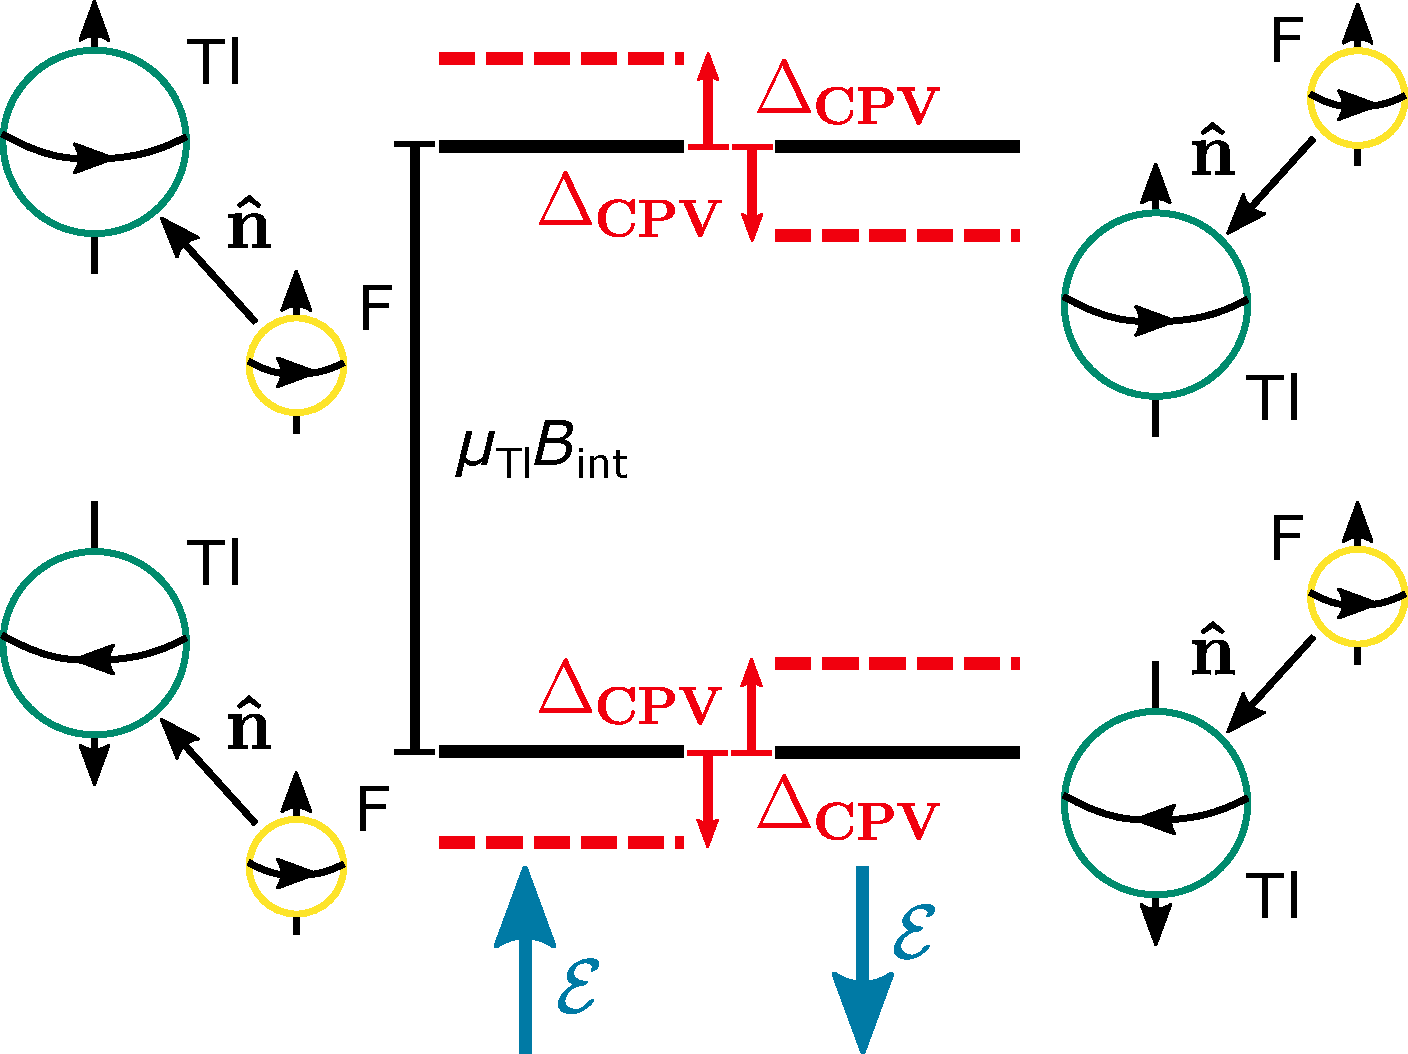
\includegraphics[width=0.48\textwidth,unit=1mm]{figs/svg/edm_levels_pdf_version.pdf}
	\caption{T-violating energy shift $\Delta_{\rm CPV} = W_SS\,\mathcal{P}$ as a result of a nonzero NSM $S$ given by the effective interaction $\mathcal{H}_\text{CPV}= W_S S\vec{I}\cdot \hat{\vec{n}}/I$ (Eq.~\ref{eq:Hamiltonian_effective_interaction}), shown for opposite orientations of the applied field $\Evec$. Here $\mu_1$ is the Tl magnetic moment and $B_1^\mathrm{int}$ is the effective internal magnetic field at the Tl nucleus due to the spin-rotation interaction.
	}
	\label{fig:edm_shift}
\end{figure}

Polar molecules can be polarized readily in laboratory-scale fields owing to their small rotational level separation ($\sim\!10^{-4}\eV$), giving them near-maximal energy shifts induced by a given Schiff moment. Thus, Sandars \cite{sandars1967measurability} suggested a molecular-beam resonance experiment could be used to probe the existence of the proton EDM, if the molecule has a heavy atom with an unpaired proton in the nucleus, such as $^{205}\mathrm{Tl}$. The value of $S$ is determined by measuring energy splittings between spin-up and -down states relative to $\left\langle \hat{\vec{n}}\right\rangle$ (which is parallel to the applied electric field $\bm{\mathcal{E}}$). This splitting will increase or decrease as $\bm{\mathcal{E}}$ (and hence $\left\langle \hat{\vec{n}}\right\rangle$) reverses, due to the interaction in Eq.~\ref{eq:Hamiltonian_effective_interaction}. The difference in level splittings is proportional to the electric polarization $\mathcal{P}$, the interaction strength $W_S$, and $S$ (Fig. \ref{fig:edm_shift}).

\CENTREX\ uses a cold beam of thallium fluoride (TlF) to measure nuclear $T$-violation due to the NSM of the $^{205}$Tl nucleus. It is a suitable system to look for $P$- and $T$-violating interactions for a number of reasons: a molecular beam of thallium fluoride can be readily obtained; many of the molecular states and transitions are known experimentally; the species is a polar diatomic molecule, enhancing the electron density gradient at the site of the nuclei (and hence $W_S$). As the thallium nucleus is heavy $\left(A=205,\,Z=81\right)$ and the NSM-induced energy shift scales $\propto A^{2/3}Z^2$, the observable effect of the Tl Schiff moment is correspondingly large \cite{sandars1967measurability, wilkening1984search}. Since the Tl nucleus contains an unpaired proton,
%the different linear combinations of underlying CPV parameters means
\CENTREX\ will be primarily sensitive to proton EDM effects, as opposed to other leading experiments which are more sensitive to the
%effects associated with neutron spin such as
neutron EDM \cite{graner2016reduced}. TlF is not very sensitive to the electron EDM due to its zero total electron spin \cite{kozlov1995parity}. 

The current best constraint on $T$-violating interactions associated with $S\left(^{205}\mathrm{Tl}\right)$ was found by Cho, Sangster and Hinds in 1991 \cite{cho1989tenfold, cho1991search}, who measured a NSM-induced frequency shift of $\Delta E = 2\Delta_{\rm CPV} = \left(1.4\pm 2.4\right)\times 10^{-4}$~Hz, consistent with zero.\footnote{Throughout, we express both frequencies and energies in linear frequency units (Hz), and all angular momentum operators are treated as dimensionless.} 
Using the effective interaction $\mathcal{H}_\text{CPV}$, the shift in the energy splitting between states with Tl spin up versus spin down, relative to the quantization axis, can be interpreted as
\begin{equation}
    \Delta E= 2 \Delta_{\rm CPV} = 2 W_S\,S\, \textrm{sgn}(\Esca) \,\mathcal{P},
    \label{eq:frequency_shift_due_to_NSM}
\end{equation}
where $W_S = 40539\,$a.u.,
polarization $\mathcal{P} = \langle\hat{\vec{n}} \cdot \hat{\Evec}\rangle = 0.547$, and the sign of $\Esca$ refers to the direction of $\Evec$ relative to a fixed quantizing axis $\hat{z}$.  This determines the Schiff moment \cite{PhysRevA.101.042501, PhysRevLett.88.073001}
\begin{equation}
    S\left(^{205}\mathrm{Tl}\right) = \left(3.6\pm 6.1\right)\times 10^{-11}\,e\,\mathrm{fm}^3.
\end{equation}
With Eq.~\ref{eq:schiff_contributions}, the following limits can be placed:
\begin{equation}
    \label{eq:prev_best_lims}
    \begin{split}
        \bar{\theta} & = \left(1.3 \pm 2.3\right)\ee{-9}, \\
        12\bar{d}_d+9\bar{d}_u & = \left(3.6\pm 6.1\right)\ee{-24}\,\mathrm{cm}, \\
        d_p          & = \left(0.9 \pm 1.5\right)\ee{-23}\,e\,\mathrm{cm},\\
        0.13g\bar{g}_0 - 0.004g\bar{g}_1-0.27g\bar{g}_2 & = \left(3.6 \pm 6.1\right)\ee{-11}.
    \end{split}
\end{equation}
\CENTREX\ aims to improve on these limits by using a cryogenic molecular beam source to achieve a cold beam with higher intensity and lower velocity spread compared to the jet source used in the previous work. Rotational cooling will be performed with optical and microwave pumping, collapsing much of the initial Boltzmann distribution into one state, greatly enhancing the number of molecules accessible for measurement. Finally, optical cycling will be used to assist state readout, resulting in near-unity detection efficiency. Fluorescence detection, compared to the hot-wire techniques used previously, allows for background-free detection if scattered light is well controlled.

\subsection{Thallium Fluoride}
\label{sec:tlf_theory}

\begin{figure}
	    % for axis breaks
    \usetikzlibrary{decorations.markings}
    \def\MarkLt{4pt}
    \def\MarkSep{2pt}
    \tikzset{
      TwoMarks/.style={
        postaction={decorate,
          decoration={
            markings,
            mark=at position #1 with
              {
                  \begin{scope}[xslant=0.2]
                  \draw[line width=\MarkSep,white,-] (0pt,-\MarkLt) -- (0pt,\MarkLt) ;
                  \draw[-] (-0.5*\MarkSep,-\MarkLt) -- (-0.5*\MarkSep,\MarkLt) ;
                  \draw[-] (0.5*\MarkSep,-\MarkLt) -- (0.5*\MarkSep,\MarkLt) ;
                  \end{scope}
              }
           }
        }
      },
      TwoMarks/.default={0.5},
    }

\begin{tikzpicture}[scale=5]

   % length of energy level diagram lines
   \def\len{.05}

   % x-position and length and x-offset of the y-axis labels
   \def\pos{-18}
   \def\lenmark{.025}
   \def\xoffset{.18}

   % x coordinates for m = -2, ... 2
   \def\xa{-4.5*\len}
   \def\xb{-2.5*\len}
   \def\xc{-0.5*\len}
   \def\xd{+1.5*\len}
   \def\xe{+3.5*\len}
   \def\xf{-6.5*\len}
   \def\xg{+5.5*\len}

   % y offset for J = 1, 2
   \def\yA{.6}
   \def\yB{\yA+.7}

   % axis
   \draw[->,TwoMarks=0.2,TwoMarks=0.6] (\xf-\len-\xoffset, -.1)
      -- (\xf-\len-\xoffset,\yB+.25) node[above, xshift = -20] {$E$ [kHz]};

   % brace position
   \def\bracePos{\xg+3*\len}

    
   % J=0 labels
   \draw [decorate,decoration={brace,amplitude=5pt,mirror,raise=4pt},yshift=0pt]
      (\bracePos,-.08) -- node (midJ0) {} (\bracePos,.08) node [black,midway,anchor=west,xshift=25] (nodeJ0) {$0$};
   \draw (\xf-\len-0.5*\lenmark-\xoffset, -.003325) node[anchor=east,below,xshift=\pos]
      {-3.325} -- (\xf-\len+0.5*\lenmark-\xoffset,-.003325) node[right,below,xshift=-\pos] {$1$};
   \draw (\xf-\len-0.5*\lenmark-\xoffset, .009975) node[anchor=east,above,xshift=\pos]
      {9.975} -- (\xf-\len+0.5*\lenmark-\xoffset,.009975) node[right,above,xshift=-\pos] {$0$};

   % J=0 lines
   \draw (\xc, -0.003325) -- (\xc+\len, -0.003325);
   \draw (\xb, -0.003325) -- (\xb+\len, -0.003325);
   \draw (\xd, -0.003325) -- (\xd+\len, -0.003325);
   \draw (\xc, 0.009975) -- (\xc+\len, 0.009975);

   % J=1 labels
   \draw [decorate,decoration={brace,amplitude=10pt,mirror,raise=4pt},yshift=0pt]
      (\bracePos,\yA-.2) -- node (midJ1) {} (\bracePos,\yA+.1) node [black,midway,anchor=west,xshift=25] (nodeJ1) {$1$};
   \draw (\xf-\len-0.5*\lenmark-\xoffset, \yA-.143745) node[anchor=east,below,xshift=\pos] {-143.745} --
      (\xf-\len+0.5*\lenmark-\xoffset,\yA-.143745) node[right,below,xshift=-\pos] {$0$};
   \draw (\xf-\len-0.5*\lenmark-\xoffset, \yA-.121506) node[anchor=east,above,xshift=\pos] {-121.506} --
      (\xf-\len+0.5*\lenmark-\xoffset,\yA-.121506) node[right,above,xshift=-\pos] {$1$};
   \draw (\xf-\len-0.5*\lenmark-\xoffset, \yA+.054446) node[anchor=east,below,xshift=\pos] {54.446} --
      (\xf-\len+0.5*\lenmark-\xoffset,\yA+.054446) node[right,below,xshift=-\pos] {$1$};
   \draw (\xf-\len-0.5*\lenmark-\xoffset, \yA+.068985) node[anchor=east,above,xshift=\pos] {68.985} --
      (\xf-\len+0.5*\lenmark-\xoffset,\yA+.068985) node[right,above,xshift=-\pos] {$2$};

   % J=1 lines
   \draw (\xc, \yA-.143745) -- (\xc+\len, \yA-.143745);
   \draw (\xc, \yA-.121506) -- (\xc+\len, \yA-.121506);
   \draw (\xb, \yA-.121506) -- (\xb+\len, \yA-.121506);
   \draw (\xd, \yA-.121506) -- (\xd+\len, \yA-.121506);
   \draw (\xc, \yA+.054446) -- (\xc+\len, \yA+.054446);
   \draw (\xb, \yA+.054446) -- (\xb+\len, \yA+.054446);
   \draw (\xd, \yA+.054446) -- (\xd+\len, \yA+.054446);
   \draw (\xc, \yA+.068985) -- (\xc+\len, \yA+.068985);
   \draw (\xb, \yA+.068985) -- (\xb+\len, \yA+.068985);
   \draw (\xd, \yA+.068985) -- (\xd+\len, \yA+.068985);
   \draw (\xa, \yA+.068985) -- (\xa+\len, \yA+.068985);
   \draw (\xe, \yA+.068985) -- (\xe+\len, \yA+.068985);

   % J=2 labels
   \draw [decorate,decoration={brace,amplitude=10pt,mirror,raise=4pt},yshift=0pt]
      (\bracePos,\yB-.27) -- node (midJ2) {} (\bracePos,\yB+.18) node [black,midway,anchor=west,xshift=25] (nodeJ2) {$2$};
   \draw (\xf-\len-0.5*\lenmark-\xoffset, \yB-.217455)
   node[anchor=east,left,yshift=-5] {-217.455}
      -- (\xf-\len+0.5*\lenmark-\xoffset,\yB-.217455) node[right,below,xshift=-\pos] {$1$};
   \draw (\xf-\len-0.5*\lenmark-\xoffset, \yB-.172936)
   node[anchor=east,left,yshift=5] {-172.936}
      -- (\xf-\len+0.5*\lenmark-\xoffset,\yB-.172936) node[right,above,xshift=-\pos] {$2$};
   \draw (\xf-\len-0.5*\lenmark-\xoffset, \yB+.105876)
   node[anchor=east,left,yshift=-5] {105.876}
      -- (\xf-\len+0.5*\lenmark-\xoffset,\yB+.105876) node[right,below,xshift=-\pos] {$2$};
   \draw (\xf-\len-0.5*\lenmark-\xoffset, \yB+.141095)
   node[anchor=east,left,yshift=5] {141.095}
      -- (\xf-\len+0.5*\lenmark-\xoffset,\yB+.141095) node[right,above,xshift=-\pos] (J2F3label) {$3$};

   % J=2 lines
   \draw (\xc, \yB-.217455) -- (\xc+\len, \yB-.217455);
   \draw (\xb, \yB-.217455) -- (\xb+\len, \yB-.217455);
   \draw (\xd, \yB-.217455) -- (\xd+\len, \yB-.217455);
   \draw (\xc, \yB-.172936) -- (\xc+\len, \yB-.172936);
   \draw (\xb, \yB-.172936) -- (\xb+\len, \yB-.172936);
   \draw (\xd, \yB-.172936) -- (\xd+\len, \yB-.172936);
   \draw (\xa, \yB-.172936) -- (\xa+\len, \yB-.172936);
   \draw (\xe, \yB-.172936) -- (\xe+\len, \yB-.172936);
   \draw (\xc, \yB+.105876) -- (\xc+\len, \yB+.105876);
   \draw (\xb, \yB+.105876) -- (\xb+\len, \yB+.105876);
   \draw (\xd, \yB+.105876) -- (\xd+\len, \yB+.105876);
   \draw (\xa, \yB+.105876) -- (\xa+\len, \yB+.105876);
   \draw (\xe, \yB+.105876) -- (\xe+\len, \yB+.105876);
   \draw (\xc, \yB+.141095) -- (\xc+\len, \yB+.141095);
   \draw (\xb, \yB+.141095) -- (\xb+\len, \yB+.141095);
   \draw (\xd, \yB+.141095) -- (\xd+\len, \yB+.141095);
   \draw (\xa, \yB+.141095) -- (\xa+\len, \yB+.141095);
   \draw (\xe, \yB+.141095) -- (\xe+\len, \yB+.141095);
   \draw (\xf, \yB+.141095) -- (\xf+\len, \yB+.141095);
   \draw (\xg, \yB+.141095) -- (\xg+\len, \yB+.141095);

   % microwave energies
   \draw[Latex-Latex] (nodeJ0) -- node[above,sloped] {13.3 GHz} (nodeJ1);
   \draw[Latex-Latex] (nodeJ1) -- node[above,sloped] {26.7 GHz} (nodeJ2);

   % approximate F1 labels
   \def\FposX{-5}
   \def\FposY{15}
   \def\FposYY{22}
   \node[xshift=\FposX] at (midJ0) {\nicefrac{1}{2}};
   \node[xshift=\FposX,yshift=-\FposY] at (midJ1) {\nicefrac{1}{2}};
   \node[xshift=\FposX, yshift=\FposY] at (midJ1) {\nicefrac{3}{2}};
   \node[xshift=\FposX,yshift=-\FposYY] at (midJ2) {\nicefrac{3}{2}};
   \node[xshift=\FposX, yshift=\FposYY] at (midJ2) {\nicefrac{5}{2}};
   \node[xshift=\FposX, yshift=47] at (midJ2) (F1label) {$F_1$};
    
   \node at (F1label -| nodeJ2) {$J$};
   \node at (F1label -| J2F3label) {$F$};

\end{tikzpicture}

	\caption{Hyperfine structure in the lowest three rotational levels in the TlF ground state $X^1\Sigma^+$, with no applied fields. Rotational energies $hBJ(J+1)$ should be added to
	%are subtracted from
	the hyperfine energy shifts indicated on the axis. Note the $(2F+1)$-fold degeneracy of each state with total angular momentum $F$, corresponding to the quantum numbers $m_F=-F,\dots,0,\dots,F$.}
	\label{fig:level_diagram}

\end{figure}

The TlF molecule is described by its electronic, vibrational and rotational motion, plus the states of the Tl and F nuclear spins. \CENTREX\ makes use of states both in the vibronic ground state, $X ^1\Sigma^+\left(\nu=0\right)$, and in an electronically excited state, $B ^3\Pi_1\left(\nu=0\right)$.  In both cases, we describe the angular momentum couplings in a Hund's case (a) basis. We typically write energy eigenstates in terms of the basis states $\ket{\eta,J,F_1,F,m_F}$. Here, $\eta$ represents the vibronic quantum numbers; $J$ is the total angular momentum excluding the nuclear spins, $\vec{F}_1 = \vec{J}+\vec{I}_\mathrm{1}$, with $I_\mathrm{1}=1/2$ for $^{205}$Tl; $\vec{F} = \vec{F}_1+\vec{I}_\mathrm{2}$ is the total angular momentum, with $I_\mathrm{2}=1/2$ for $^{19}$F; and $m_F$ is its projection along a quantization axis in the lab frame. Field-free eigenstates are close to these basis states in the ground $X ^1\Sigma^+$ state.  In the $B ^3\Pi_1$ state, strong hyperfine interactions significantly mix states with different $J$ and $F_1$ values. Hence, we describe these eigenstates with the modified notation $\ket{\eta',\widetilde{J}' ,\widetilde{F}_1^\prime,F',m_F'}$, where $\widetilde{J}'$ and $\widetilde{F}_1^\prime$ correspond to the largest component in their basis-state decomposition; the primes indicate that the ket refers to the excited state $B ^3\Pi_1$.

Molecules in the beam are assumed to be in the vibronic ground state, since the beam temperature is much lower than the energy scales associated with the electronic and vibrational excitations. However, even at cryogenic temperatures, there is a Boltzmann distribution over many rotational and nuclear spin states. The dominant term in the energy of rotational/spin levels in the $X ^1\Sigma^+$ state is due to rotation; the mean energy of states with quantum number $J$ is $E_\mathrm{rot}=BJ(J+1)$, where $B\approx 6.67\GHz \approx 0.3\kelvin\,\kB$, where $\kB$ the Boltzmann constant.\footnote{In Ramsey et al.\ \cite{wilkening1984search}, the symbol $B$ denotes the rotational constant in equilibrium position, i.e., there $B\equiv B_\text{e}$. However, the effective $v=0$ rotational constant, $B_0$, is more relevant to \CENTREX. To first order in the Dunham expansion \cite{huber2013molecular}, $B_0=B_\text{e}-\alpha_\text{e}/2$. With $B_\text{e}$ and $\alpha_\text{e}$ from the NIST database \cite{afeefy2011nist}, we find $B_0$. We define the symbol $B\equiv B_0$; its value is shown in Table~\ref{tab:hyperfine_hamiltonian}.}

Hyperfine interactions split sublevels with different $F$ values ($F=J-1,J,J, J+1$, except $F=0,1$ only for $J=0$) in each rotational state. Thus, each rotational level has $4(2J+1)$ magnetic sublevels. %including nuclear spins.
Including rotation, spin-rotation and spin-spin interactions, plus interactions with external electric $(\Evec)$ and magnetic $(\Bvec)$ fields, the system is described by the effective Hamiltonian \cite{wilkening1984search}
\small
$\mathcal{H}_\text{TlF} = \mathcal{H}_\text{rot}+\mathcal{H}_\text{sr}+\mathcal H_\text{ss} + \mathcal H_\text{S}+\mathcal H_\text{Z}$, 
\normalsize
where
\begin{equation} 
    \label{eq:hyperfine_hamiltonian}
    \begin{split}
        \mathcal H_\text{rot} & = B \vec{J}^2 \\
        \mathcal H_\text{sr}&=c_1(\vec I_1\cdot\vec J)+c_2(\vec I_2\cdot\vec J), \\
        \mathcal H_\text{ss}&=c_3 T^2(\vec C)\cdot T^2(\vec I_1, \vec I_2)+c_4(\vec I_1\cdot\vec I_2), \\
        \mathcal H_\text{S}&=-\vec\mu_e\cdot\vec \Evec,\\
        \mathcal H_\text{Z}&=-\frac{\mu_J}{J}(\vec J\cdot\vec \Bvec)-\frac{\mu_1}{I_1}(\vec I_1\cdot\vec \Bvec)-\frac{\mu_2}{I_2}(\vec I_2\cdot\vec \Bvec).
    \end{split}
\end{equation}
Here, the first term in the spin-spin interaction ($\mathcal H_\text{ss}$) contains the scalar product of two rank-2 tensors: one constructed from the modified spherical harmonics $\vec C$, and one from $\vec{I}_1$ and $\vec{I}_2$ \cite{brown2003rotational}. (The matrix elements diagonal in $J$ of this term are given in \cite{wilkening1984search}.)  The hyperfine parameters $c_1,c_2,c_3,c_4$, rotational constant $B$, magnetic moments $\mu_J,\mu_1,\mu_2$, and molecule-frame electric dipole moment $\mu_e$ are all known from previous measurements; their values are given in  Table~\ref{tab:hyperfine_hamiltonian}. A level diagram of low-lying states in the absence of applied fields is shown in Fig.~\ref{fig:level_diagram}.

\begin{table}
    \small
    \setlength\extrarowheight{3pt}
    \rowcolors{2}{white}{gray!25}
	\centering
	\caption{Constants describing rotational, hyperfine, Zeeman, and Stark interactions in the effective TlF ground-state  Hamiltonian (Eq.~\ref{eq:hyperfine_hamiltonian}). All values taken from Ramsey et al.\ \cite{wilkening1984search}, except for $B$ (see Sec. \ref{sec:tlf_theory}).}
	\label{tab:hyperfine_hamiltonian}
	\begin{tabular}{r@{\hspace{5pt}}c@{\hspace{5pt}}l@{\hspace{5pt}}l | r@{\hspace{5pt}}c@{\hspace{5pt}}l@{\hspace{5pt}}l}
    	\toprule
		$B$ & = &           $6.66733$ &     GHz &       $\mu_e$ & = & $4.2282(8)$ &     Debye \\
		$\mu_J$ & = &       $35(15)$ &      Hz/G &      $c_1$ & = & $126.03(12)$ &    kHz \\
		$\mu_1^{205}$ & = & $1.2405(3)$ &   kHz/G &     $c_2$ & = & $17.89(15)$ &     kHz\\
		$\mu_1^{203}$ & = &  $1.2285(3)$ &   kHz/G &     $c_3$ & = & $0.70(3)$ &       kHz \\
		$\mu_2$ & = &      $2.00363(4)$ &  kHz/G  &    $c_4$ & = & $-13.30(72)$ &    kHz \\
		\bottomrule
	\end{tabular}
\end{table}

%%%%%%%%%%%%%%%%%%%%%%%%%%%%%%%%%%%%%%%%%%%%%%55%%%%%%%%%%%%%%%
In \CENTREX, lasers are tuned to $X^1\Sigma^+(\nu=0)\rightarrow B^3\Pi_1\left(\nu=0\right)$ transitions in order to manipulate and read out ground state hyperfine and rotational sublevels. Details of the $B ^3\Pi_1$ state structure are given in \cite{norrgard2017hyperfine,PhysRevA.101.042506}.  Here, only a few main features of the $B$ state substructure are important.  First, the $B$ state hyperfine splittings are very large ($\gtrsim 100\MHz$) compared to the natural linewidth of the transition ($\gamma_B \approx 1.6\MHz$), which is in turn much larger than the ground-state hyperfine splittings ($c_j \lesssim 100\kHz$). This means that hyperfine structure is fully resolved in the excited state, and entirely unresolved in the ground state. Hence, optical transitions in TlF drive a large manifold of ground-state hyperfine levels (with a given value of $J$) to a single hyperfine state with (nominal) quantum numbers $\tilde{J},\tilde{F}_1$ and exact quantum number $F$. Another important feature of the $B$ state is that its matrix of Franck-Condon factors (FCFs) for decay to the $X$ state is extremely diagonal \cite{hunter2012prospects}, such that $\sim\! 99\%$ of the time, the $B(v=0)$ vibronic state decays back to the vibronic ground state $X(v=0)$.  This enables optical pumping and optical cycling with little loss.  However, the mixing of $J$ and $F_1$ by the strong $B$-state hyperfine interaction substantially modifies rotational selection rules in $B-X$ decays, and must be taken into account when describing optical excitation and emission in TlF.

\subsection{TlF in \texorpdfstring{$\Esca$}{E}-fields}
\label{sec:TlF_in_E_fields}

\begin{figure*}
	\centering
	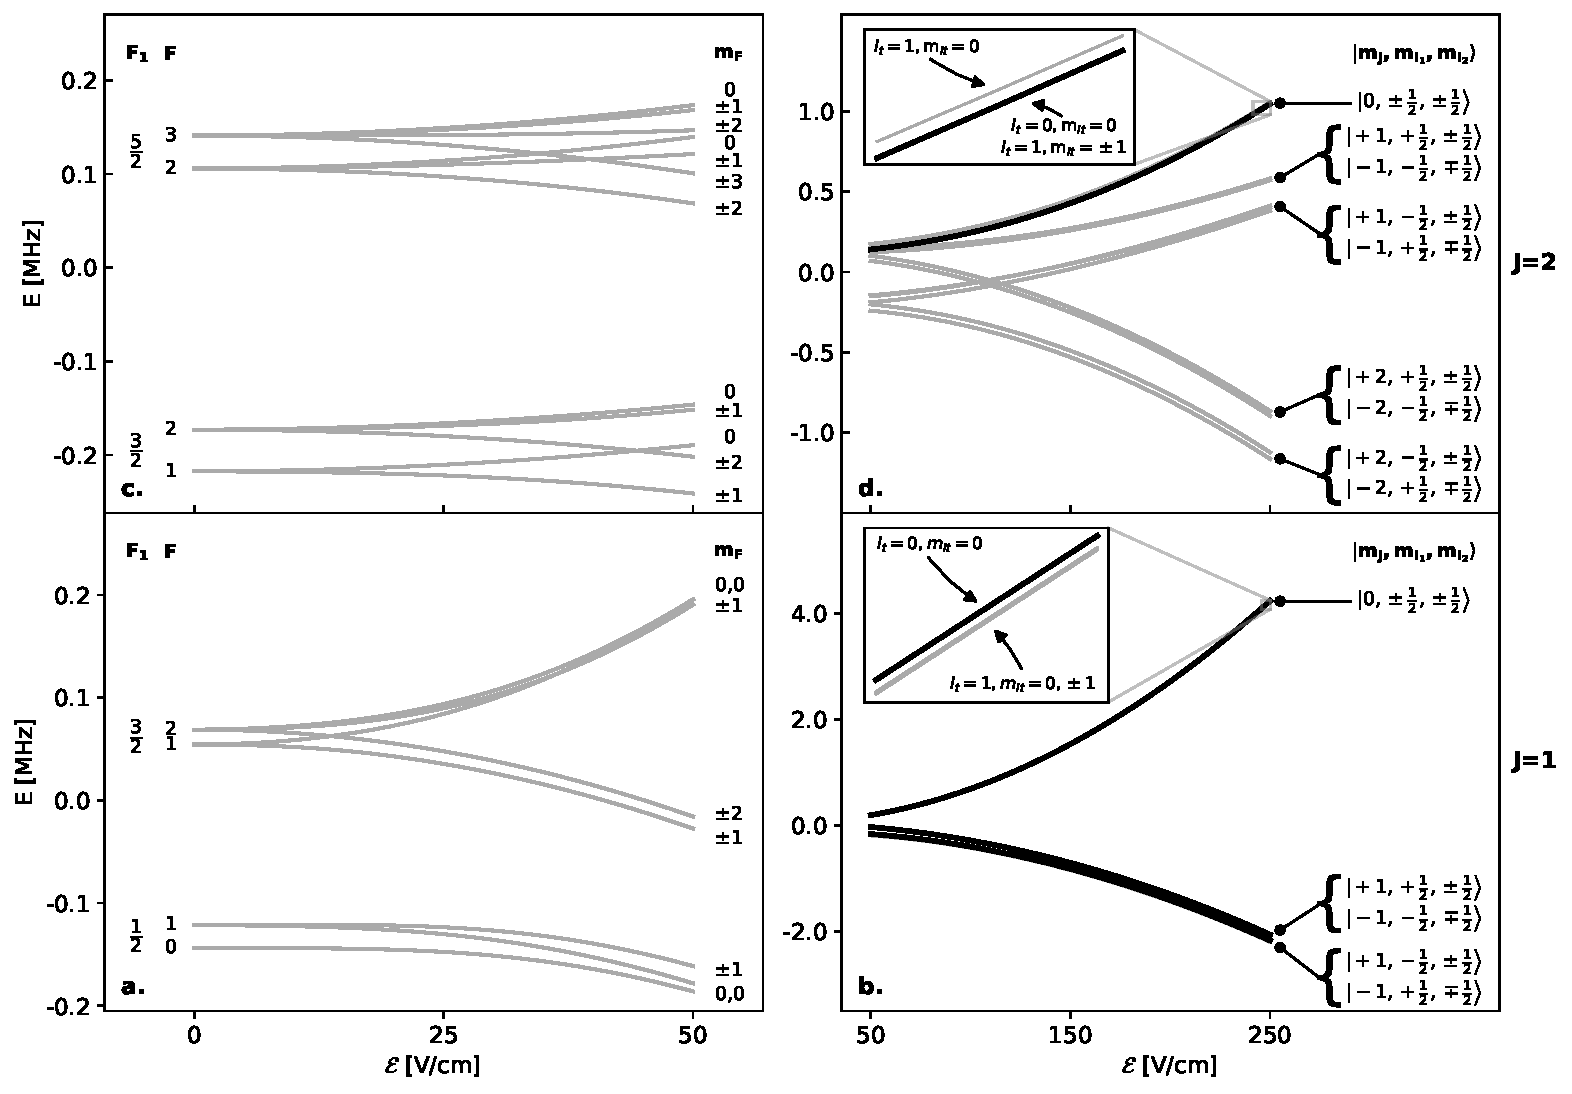
\includegraphics[width=\textwidth]{figs/matplotlib/low_to_mid_field.pdf}
	\caption{Overview of the energy eigenstates for changing $\Esca$-field magnitudes. The low-field regime, where $\Delta E_{\rm S} \ll E_{\rm hf}$, where energy eigenstates retain $J$, $F$, and $F_1$ as approximate quantum numbers is shown in \part{a} for $J=1$ and \part{c} for $J=2$. The mid-field regime, where $E_{\rm hf} \ll \Delta E_{\rm S} \ll E_{\rm rot}$, where both $J$ and $m_J$ are approximate quantum numbers is shown in \part{b} for $J=1$ and \part{d} for $J=2$. States used in \CENTREX\ are shown in bold.}
	\label{fig:low_to_mid_field}
\end{figure*}

\begin{figure}
	\centering
	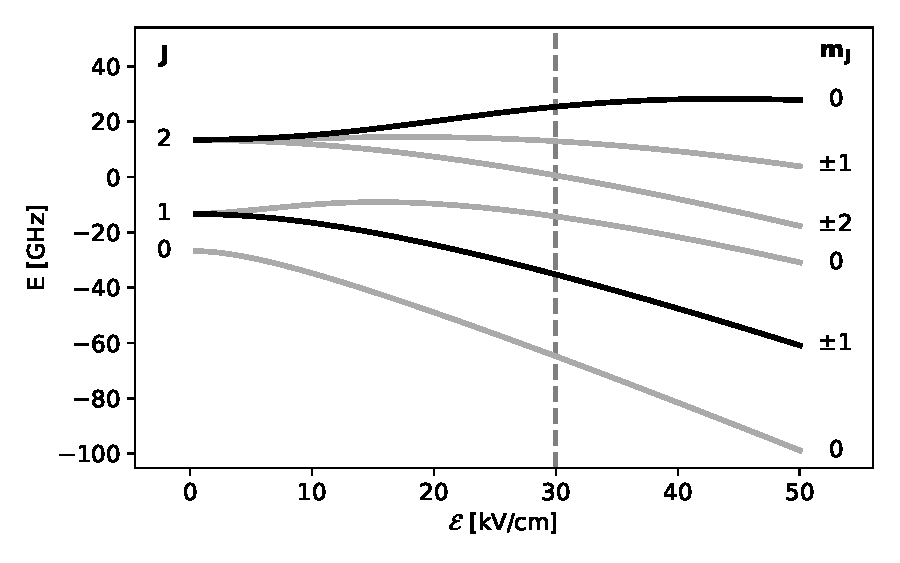
\includegraphics[width=\textwidth/2]{figs/matplotlib/low_to_high_field.pdf}
	\caption{Evolution of the energy eigenstates of the TlF Hamiltonian (Eq. \ref{eq:hyperfine_hamiltonian}) for $\Esca$ ranging from $0\,$V/cm to $50\,$kV/cm, for $J=0,1,2$. States used in \CENTREX\ are shown in bold. Hyperfine structure is unresolved in this plot.}
	\label{fig:low_to_high_field}
\end{figure}

Throughout most of the \CENTREX\ apparatus, TlF molecules experience a non-zero $\Esca$-field and (nominally) zero $\Bsca$-field.
The character of the energy eigenstates changes significantly depending on the $\Esca$-field magnitude, which varies dramatically between stages of the experiment. Hence, it is useful to describe the energy eigenstates of the TlF electronic ground state in different regimes of $\Esca$-field strength (with $\Bsca = 0$), as defined by the ratio of Stark shifts, $\Delta E_{\rm S} = \langle \mathcal{H}_{\rm S}\rangle \sim \mu_e^2 \Esca^2/B$, to the strength of hyperfine interactions, $E_{\rm hf} = \langle \mathcal{H}_{\rm sr} + \mathcal{H}_{\rm ss}\rangle \sim c_j$, or rotational energies, $E_{\rm rot} = \langle \mathcal{H}_{\rm rot}\rangle \sim B$. In all regimes, the total angular momentum projection $m_F$ along 
a space-fixed quantization axis $\hat{z}$ (always defined such that $\Evec$ is very nearly parallel to $\hat{z}$), is an exact quantum number.

In the low-field regime, where $\Delta E_{\rm S} \ll E_{\rm hf}$, energy eigenstates retain $J$, $F$, and $F_1$ as approximate quantum numbers. 
In the mid-field regime, where $E_{\rm hf} \ll \Delta E_{\rm S} \ll E_{\rm rot}$, both $J$ and $m_J$ are approximate quantum numbers. 
Here, the tensor part of the Stark shifts gives rise to energy splittings between levels with different values of $|m_J|$ that are comparable in size to the scalar shifts, i.e., of order $\Delta E_{\rm S}$.  Thus, when $m_J\neq 0$, $\vec{J}$ is strongly coupled to $\Evec$ (and hence to the molecular axis $\vec{\hat{n}}$) by this Stark interaction. In this case, each nuclear spin is coupled to $\vec{J}$ (and thus also to $\Evec$) by the spin-rotation interactions of $\mathcal{H}_{\rm sr}$. Hence, here $m_{I_1}$ and $m_{I_2}$ are approximate quantum numbers. By contrast, in states where $m_J=0$ (including when $J=0$) in this regime, $\left\langle \mathcal{H}_{\rm sr}\right\rangle$ vanishes to first order, and the nuclear spins do not couple to $\vec{J}$ and $\Evec$. However, the nuclear spins remain coupled to each other via the spin-spin interaction $\mathcal{H}_{\rm ss}$.  So, here the total nuclear spin $\vec \It = \vec I_1 + \vec I_2$ and its projection $m_{\It}$ are approximate quantum numbers in addition to $J$ and $m_J=0$. 
Finally, in the high-field regime where $E_{\rm hf} \ll E_{\rm rot} \lesssim \Delta E_{\rm S}$, $J$ states are strongly mixed, and separations between $m_J$ states are on the order of $E_{\rm rot}$. Here, eigenstates are defined by the same approximate quantum numbers as in the mid-field regime, aside from $J$. We refer to these strongly mixed states with the label $\widetilde{J}$, which corresponds to the value of $J$ that any given state connects to adiabatically, if the $\Esca$-field is reduced.
Table \ref{tab:E_field_regimes} summarizes the different regimes and associated eigenstates.  
\begin{table*}[t]
    \centering
    \def\colseplarge{4ex} % should only be used in this table
	\begin{tabular}{@{}r@{\hspace{\colseplarge}}r@{$\,\Delta E_{\rm S}\,$}l@{\hspace{\colseplarge}}r@{$\,\Esca\,$}l@{\hspace{\colseplarge}}>{\raggedright\arraybackslash}m{4cm}@{}}
    	\toprule
    	Regime & \multicolumn{2}{c}{Definition} & \multicolumn{2}{c}{Field strength} & Approx. eigenstates \\
		\midrule
		 Low
		 & & $\ll E_{\rm hf}$
		 & & $\lesssim 50 \Vcm$
		 & $\ket{J,F_1,F,m_F}$ \\\addlinespace[2ex]
		 %
	     Mid
	     & $E_{\rm hf} \ll$ & $\ll E_{\rm rot}$
	     & $50 \Vcm \ll$ & $\lesssim 5 \kVcm$
	     & $\ket{J,m_J \neq 0}\ket{m_{I_1},m_{I_2}}$ 
	       $\ket{J,m_J=0}\ket{\It,m_{\It}}$ \\\addlinespace[2ex]
	     %
	     High
	     & $E_{\rm hf} \ll E_{\rm rot} \lesssim$ &
	     & $5\kVcm \ll$ &
	     & $\ket{\widetilde{J},m_J\neq 0} \ket{m_{I_1},m_{I_2}}$
	       $\ket{\widetilde{J},m_J=0}\ket{\It,m_{\It}}$ \\
		\bottomrule
	\end{tabular}
	\caption{Regimes of electric field strength and associated eigenstates in TlF.}
	\label{tab:E_field_regimes}
\end{table*}


Figure \ref{fig:low_to_mid_field} shows how the relevant energies and eigenstates evolve from the low-field to the mid-field regime for $J=1$ and $J=2$ states.  Bold curves are states directly relevant to \CENTREX. Figure \ref{fig:low_to_high_field} shows a zoom out of states up to $J=2$ from low to high fields.

The $^{205}$Tl NSM measurement is carried out in $\tilde{J} = 1,\, m_J = \pm1$ states of TlF at large electric field $\mathcal{E} = 30$ kV/cm. This choice of states takes advantage of the structure of TlF in electric fields, in two ways. First, the observable energy shift associated with $S$, $\Delta E$, scales linearly with the degree of polarization $\mathcal{P}$ of the TlF molecule (Eq. \ref{eq:frequency_shift_due_to_NSM}). An electric field more easily polarizes states with low $J$, since $\mathcal{P}$ arises from mixing between states with different parity and thus different $J$; these states are closest together when $J$ is small. Additionally, as discussed in Sec. \ref{Sec:InternalComagnetometry}, certain dangerous systematic errors in the NSM measurement are dramatically suppressed in the presence of a strong spin-rotation interaction (later referred to as an effective intra-molecular magnetic field). This requires $m_J \neq 0$. The $\tilde{J} = 1,\, m_J = \pm1$ states hence provide the best combination of sensitivity and systematic error suppression in TlF.\footnote{$|\mathcal{P}|$ is larger in the $J=0,m_J = 0$ states, given the same $\Esca$-field value. Hence, the NSM gives larger energy shifts there. However, in these states where $m_J = 0$, the effective intra-molecular magnetic field vanishes.}
\paragraph{Sampling CF data.} Sampling in CF-data has been a popular choice for three major scenarios. Most prominently, sampling is used for mining hard-negatives while training recommendation algorithms. Some popular approaches include random sampling; using the graph-structure % to find the hardest negatives 
\cite{pinsage, eclare}; and ad-hoc techniques like similarity search \cite{slice}, stratified sampling \cite{sampling_cf_nn}, \etc % On the other hand, 
Sampling is also generally employed for evaluating recommendation algorithms by estimating expensive to compute metrics like Recall, nDCG, \etc \cite{sampled_metrics, castells_sampling}. Finally, sampling is also used to create smaller sub-samples of 
% the \emph{entire} data 
a big dataset
for reasons like fast experimentation, benchmarking different algorithms, privacy concerns, \etc However, the consequences of different samplers on any of these downstream applications is under-studied, and is the main research interest of this paper. 

\paragraph{Coreset selection.} Closest to our work, a coreset is loosely defined as a subset of data-points that maintains a similar ``quality'' as the full dataset for subsequent model training. Submodular approaches try to optimize a function $f : \mathbf{V} \mapsto \mathcal{R}_+$ which measures the utility of a subset $\mathbf{V} \subseteq \mathbf{X}$, and use it as a proxy to select the best coreset \cite{coreset_1}. More recent works treat coreset selection as a bi-level optimization problem \cite{coreset_bilevel, coreset_bilevel_2} and directly optimize for the best coreset for a given downstream task. Selection-via-proxy \cite{svp} is another technique which employs a base-model as a proxy to tag the importance of each data-point. Note, however, that 
% all of the discussed 
most existing
coreset selection approaches were designed primarily for classification data, whereas adapting them for CF-data is non-trivial because of: (1) the inherent data heterogeneity; the (2) wide range of recommendation metrics; and (3) the prevalent missing-data characteristics.

\paragraph{Evaluating sample quality.} The quality of a dataset sample, if estimated correctly is of high interest for various applications. Short of being able to evaluate the ``true'' utility of a sample, one generally resorts to either retaining task-dependent characteristics \cite{evaluate_sample_quality_1} \emph{or} employing universal, handcrafted features like a social network's hop distribution, eigenvalue distribution, \etc \cite{large_graphs} as meaningful proxies. Note that evaluating the sample quality with a limited set of handcrafted features might introduce bias in the sampled data, depending on the number and quality of such features.

\section{Methodology}
\begin{figure*}[t]
    \centering
    \scalebox{0.28}{
    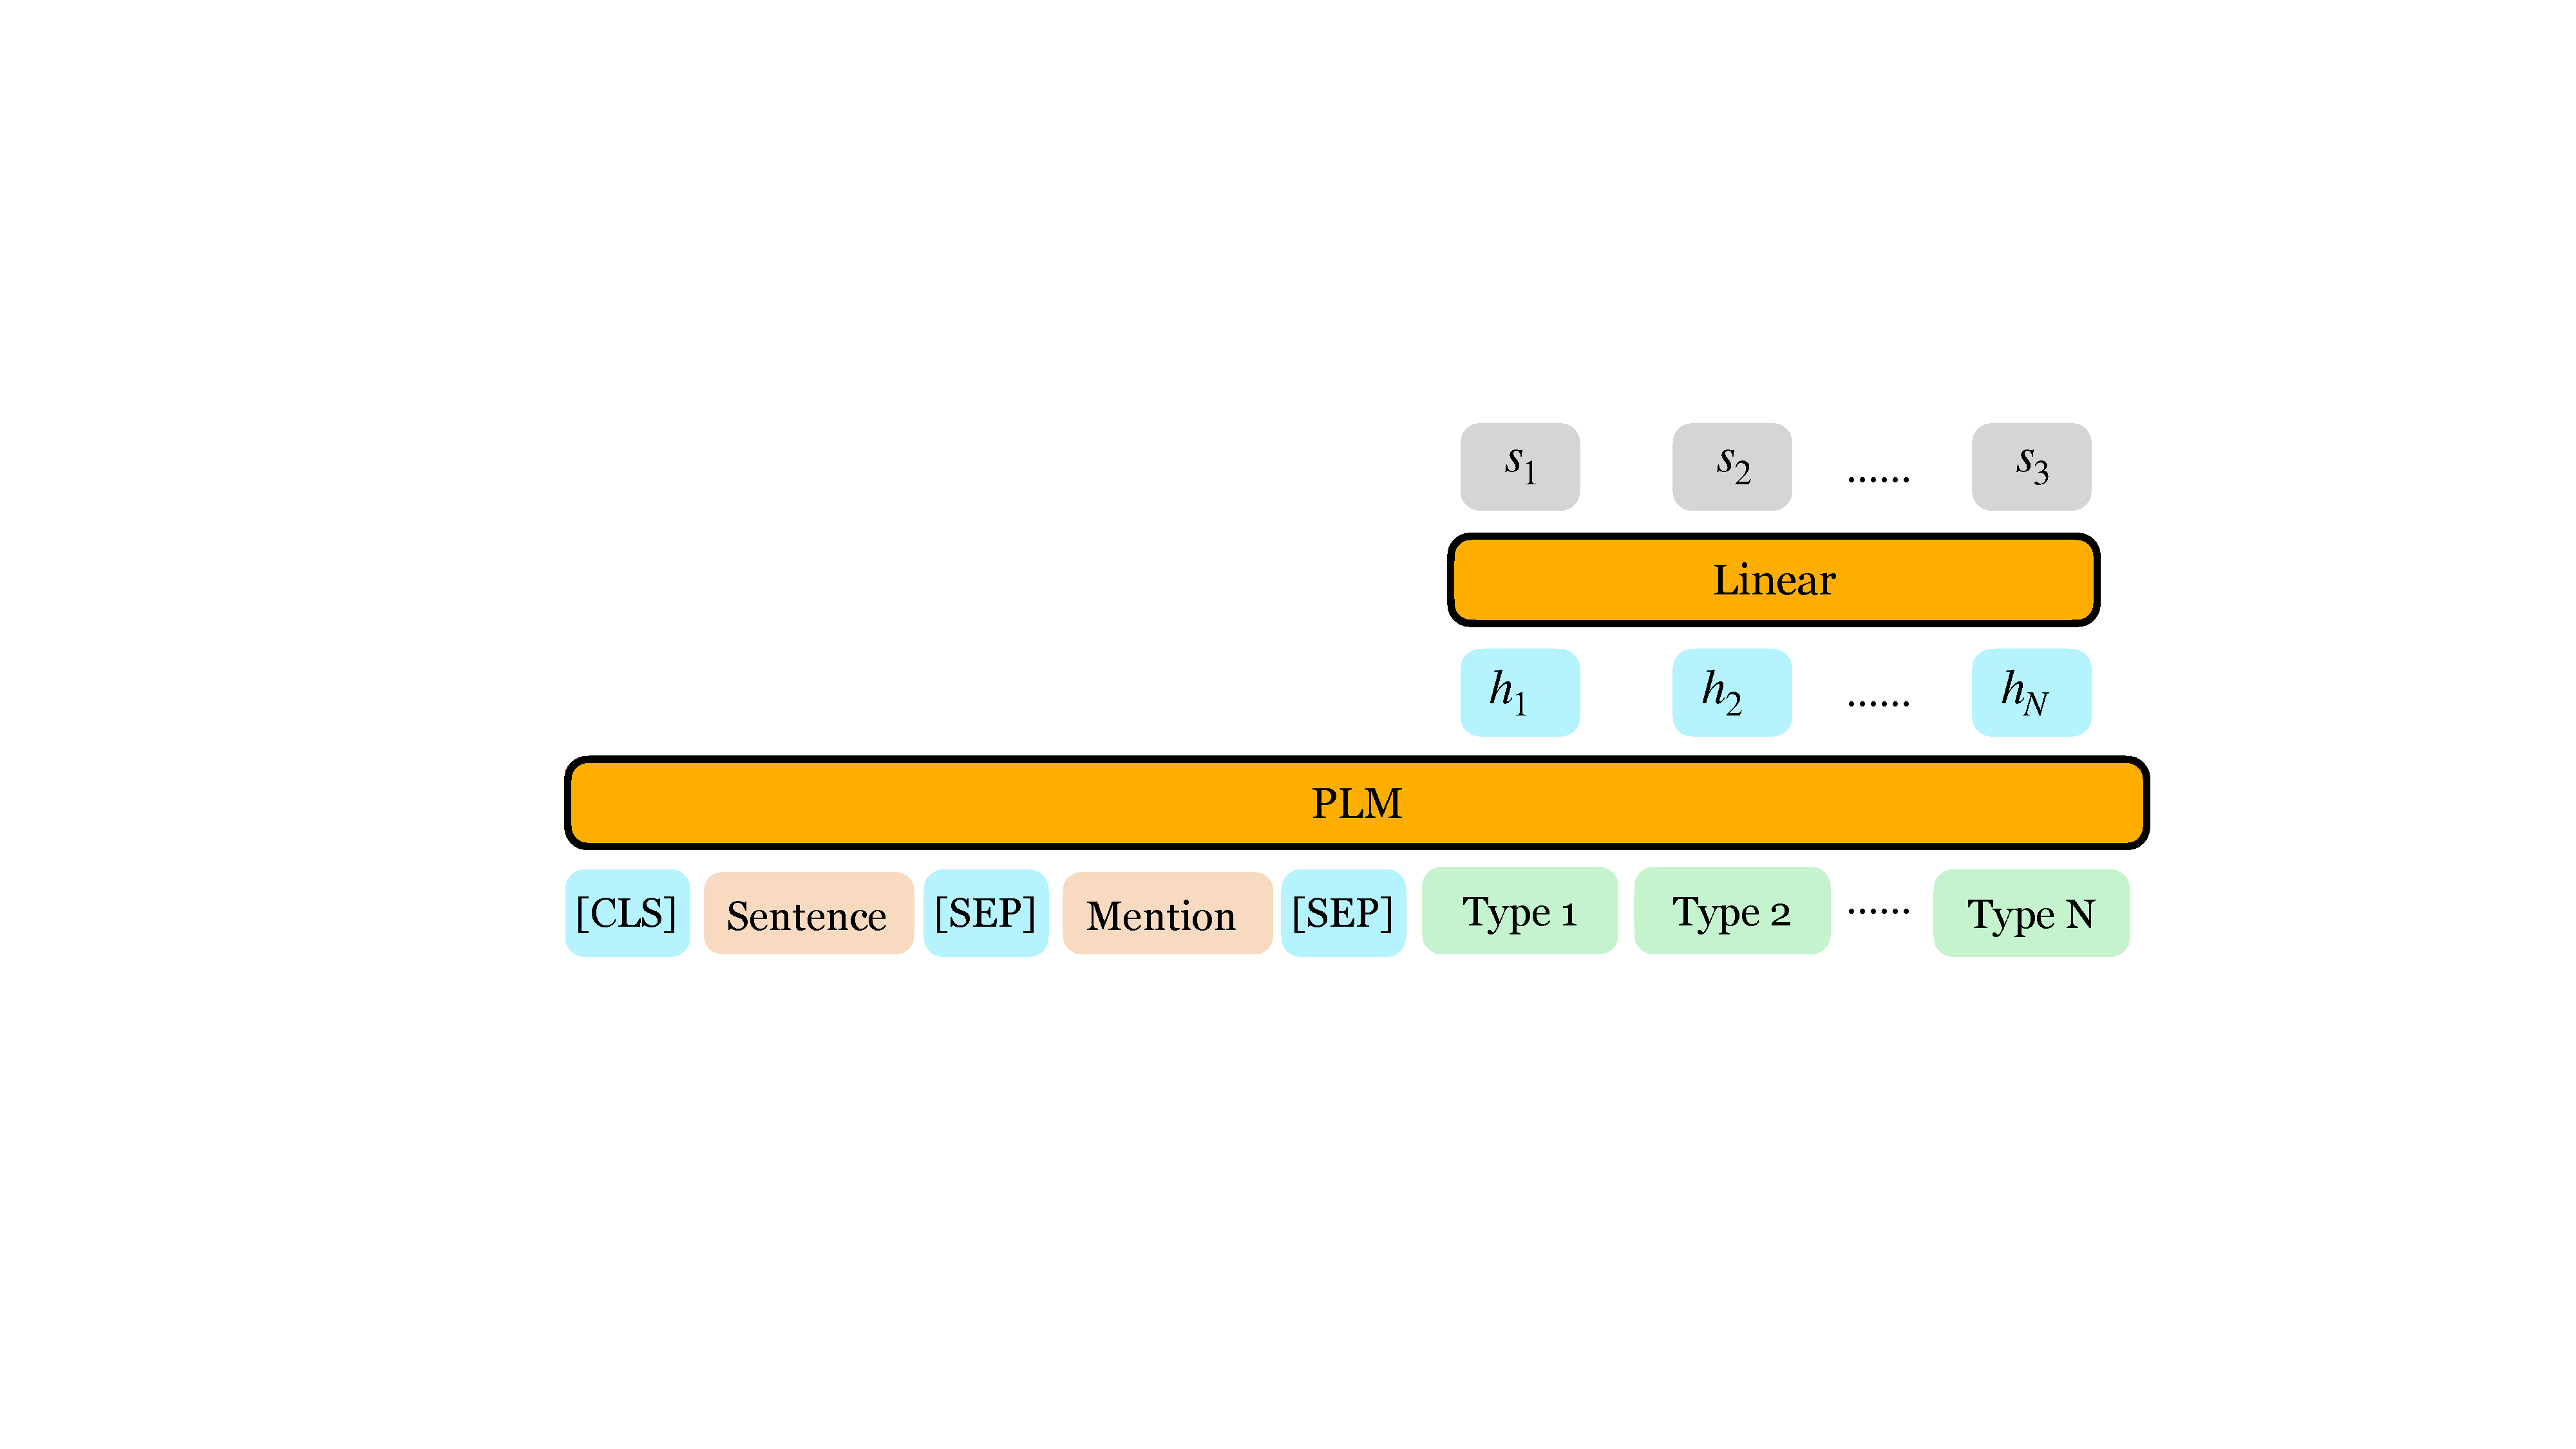
\includegraphics{src/img/ccf_model.pdf}}
    \caption{Multi-candidate cross-encoder (MCCE).}
    \label{fig:ccf}
\end{figure*}
Inspired by techniques in information retrieval \cite{ir} and entity linking \cite{wu2019zero}, we decompose the training and inference of UFET into three stages as illustrated in Figure \ref{fig:paradigm}: (1) Recall stage to reduce the type candidate size (e.g., from $N=10k$ to $K=100$) while guaranteeing the recall rate by an efficient MLC model. (2) Expand stage to incorporate lexical information using exact matching and weak supervision \cite{mlmet} from large pretrained language models such as BERT-Large \cite{bert} to improve recall rate. (3) Filter stage to filter the expanded type candidates to obtain final prediction. For the filter stage, we propose an efficient model: Multi-Candidate Cross-Encoder (MCCE) to concurrently encode and filter type candidates of a given mention with only a single forward pass. 
\subsection{Recall Stage}
To prune the type candidates set, we train a very efficient MLC model introduced in Sec. \ref{sec:mlc} and select the model based on the recall rate (e.g. recall@64) on the development set. Then we use it to infer the top $K_1$ (typically less than 256) candidates $\mathcal{C}_i^R$ for each data point $(m_i, c_i)$ for train, development, and test set. We compare MLC with a widely-used baseline model BM25 \cite{bm25} and show its advantages in Sec. \ref{sec:recall}. 
% There are other options (e.g., Bi-Encoder \cite{wu2019zero}) for the recall model. However, we choose MLC because it is easy to optimize and has the fastest inference speed\footnote{MLC model can be categorized as a simple Bi-Encoder that uses embedding to encode types.}.
\subsection{Expand Stage}
Due to the lack of training data per type, we found that the MLC we used in the recall stage easily overfits the train set, and is hard to predict the types that only appear in the development and test set. In {\bf \textsc{UFET}} dataset, 30\% of the types in the development set are unseen. To this end, we utilize lexical information using exact match and weak supervision from the masked language model (MLM) to expand the recalled candidates. Both exact match and MLM are able to recall unseen type candidates without any training. 
\paragraph{Exact Match} MLC and Bi-Encoder recall candidates by dense representations. They are known weak at identifying and utilizing the lexical matching information between the input and types \cite{matching_info1, matching_info2}. However, 
 types are free-formed in UFET (e.g., \textit{president, businessman}), and are very likely to appear in the context or mention (e.g., the mention is \textit{`the \textbf{president} Joe Biden'}). To this end, we first find all nouns in the context and mention by NLTK\footnote{nltk.tag package \url{https://www.nltk.org}} POS tagger and normalize their forms, then we recall types that exactly matched with these nouns.
\paragraph{Weak Supervision from MLM} Inspired by recently prompt-based methods for entity typing \cite{ding2021prompt, dfet}, we recall candidates by asking PLMs to fill masks in prompts. Suppose a type $y_j \in \mathcal{Y}$ can be tokenized into $l$ subwords $w_1, \cdots w_l$. To score $y_j$ given $m_i, c_i$, we first formulate the input as in Figure \ref{fig:prompt_recall}.
\begin{figure}[h]
    \centering
    \scalebox{0.2}{
    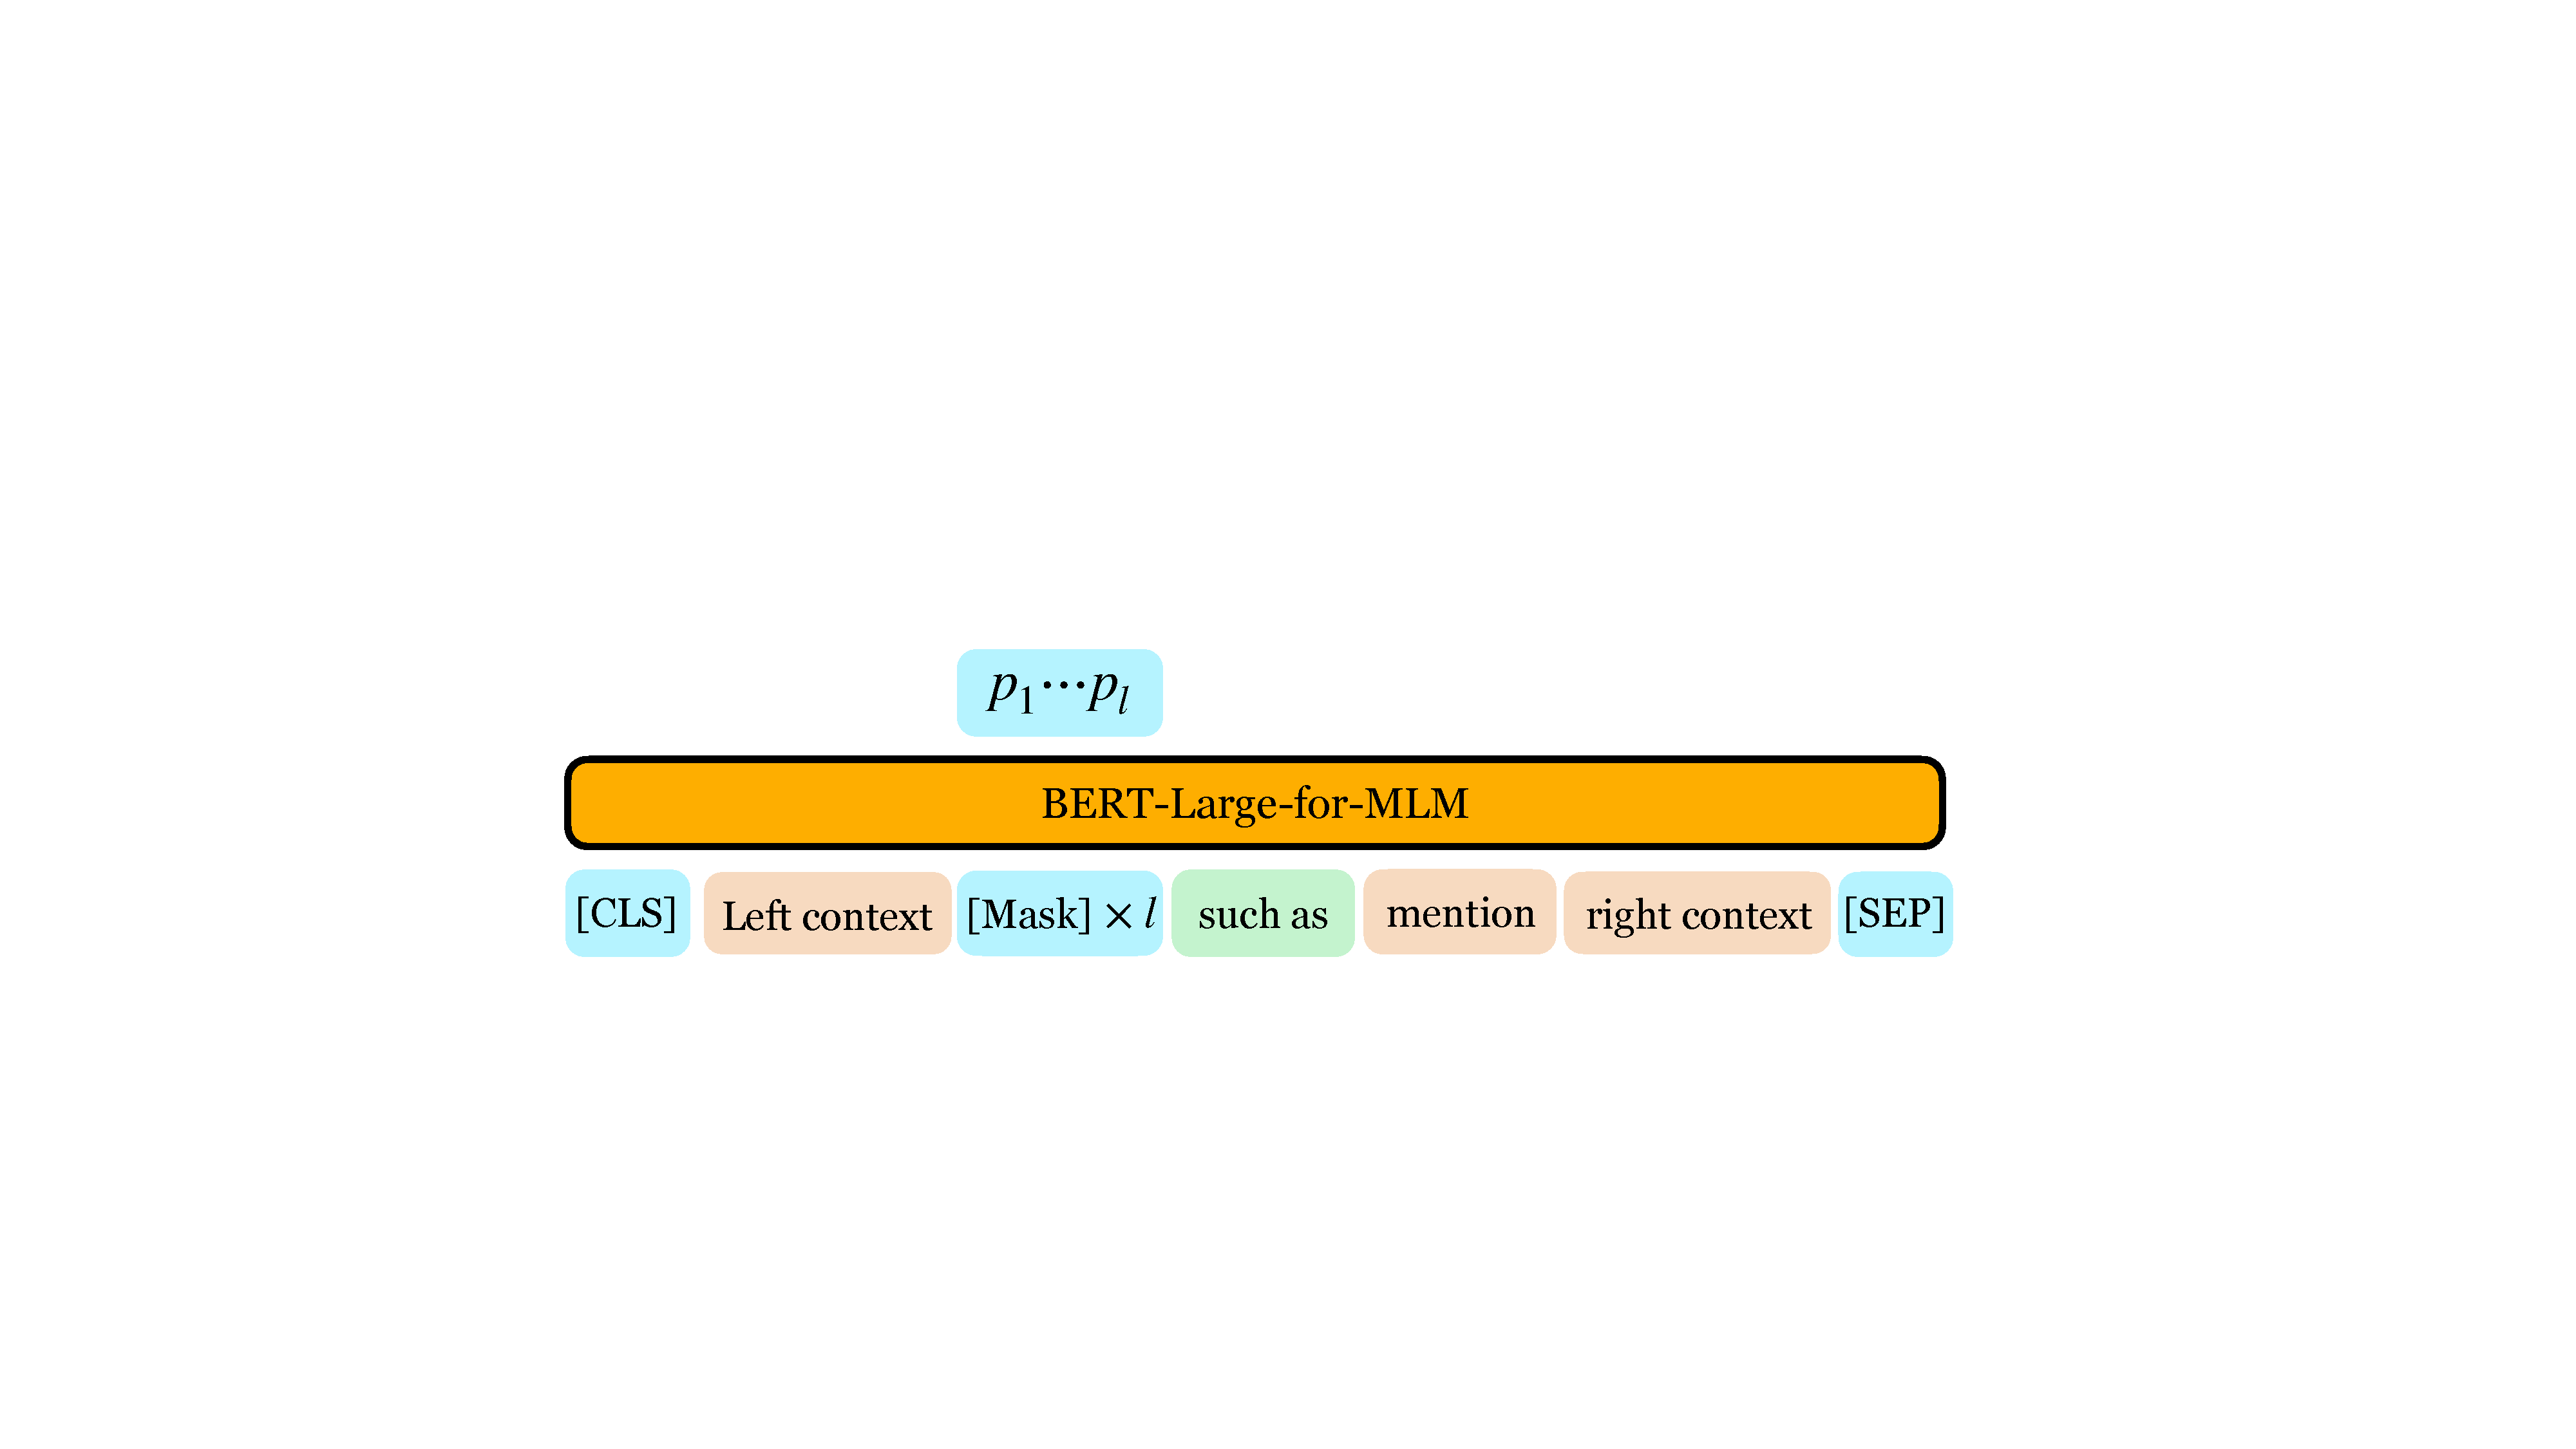
\includegraphics{src/img/prompt_recall.pdf}}
    \caption{Recall from MLM using prompts.}
    \label{fig:prompt_recall}
\end{figure}
where $c_i^l, c_i^r$ are left and right context of $m_i$, and \texttt{`such as'} is the template we use to induce types. The input is then fed into BERT-large-uncased\footnote{We use the PLM from \url{https://huggingface.co}} for masked language model to obtain the probabilities of subwords, the score of $y_j$ is calculated by $ s^{MLM}_{j} = (\sum_{n=1}^l \log p_n)/l$, where $p_l$ denotes the probability of subword $w_l$ predicted by the PLM. We rank all types by enumerating all possible $l$ and recall $K_2$ additional candidates that haven't been recalled by the recall stage and exact match. We found that the expand stage improves recalls and contributes to the performance in Sec. \ref{sec:exp_expand}.
\subsection{Filter Stage}
In the filter stage, we use the recall and expand method introduced above to efficiently generate type candidates $\mathcal{C}_i$ for data in the train, development, and test set. For training, $\mathcal{C}_i$ is used to produce positive and hard negative type candidates. For inference, $\mathcal{C}_i$ is the candidate pool for the trained filter models. Let $|\mathcal{C}_i|=K$ and $K$ is typically less than 256. 
\subsubsection{CE} A trivial idea is to train a CE model introduced in Sec. \ref{sec:vanilla_ce} to filter $\mathcal{C}_i$ instead of filtering the whole type set $\mathcal{Y}$. The positive type $y^{+}$ and negative $y^{\_}$ type are both sampled from $\mathcal{C}_{i}$ and are used for calculating marginal ranking loss. To infer types, we also recall and expand $K$ candidates and score these candidates by $K$ forward passes to predict types. As $K << |\mathcal{Y}|$, CE with our Recall-Expand-Filter paradigm is much faster than vanilla CE. However, it's still inefficient compared to MLC-like models that concurrently predict scores of all types in a single forward pass. For faster inference and training, we propose multi-candidate cross-encoders ({\bf \textsc{\name}}) and introduce them in the next section.

\section{Multi-Candidate Cross-Encoder (\name)}
\label{sec:ccf}
 In this section, we introduce {\bf \textsc{\name}} for filtering candidates in one forward pass and propose several variants. 
\subsection{Overall Introduction of \name}
As shown in Figure \ref{fig:ccf}, compared to CE that concatenates one candidate at a time, {\bf \textsc{\name}} models concatenate all candidates in $\mathcal{C}_i$ with the mention and context. The input is then fed into the PLM to obtain the hidden states of each candidate as their representation. Finally, we use an MLP to concurrently score all candidates.
\begin{equation}
\begin{aligned}
\bm{h}_{1:K}  &= \texttt{PLM}(\texttt{[CLS]} \ c_i \ \texttt{[SEP]}\  m_i \ \texttt{[SEP]} \ t_{1:K} \ )  \\
\bm{s}_{1:K}  &= \texttt{Linear}(\bm{h}_{1:K}) 
\end{aligned}
\end{equation}
where $t_{1:K}$ is the short for $t_1, \cdots, t_K$, and $t_j \in \mathcal{C}_i$. Similarly, $\bm{h}_{1:K}$ and $s_{1:K}$ are hidden representations and scores of corresponding candidates respectively. 

\paragraph{Training and Inference} For training, we found that all positive types are ranked very high in the training candidates, which is not the case for the development and test data. To prevent the filter model from overfitting the order of training candidates and only learning to predict the first several candidates, we keep permuting type candidates during training. Same as the MLC model mentioned in Sec. \ref{sec:mlc}, we use the Binary Cross-Entropy loss as the training objective and tune a threshold of probabilities on the development set for inference.

In the next subsection, we discuss different model configurations of {\bf \textsc{\name}} regarding the input formats of candidates and attention mechanisms.

\subsection{Different Input Formats of Candidates}
\paragraph{Average of type sub-tokens} We treat each type $t_j \in \mathcal{Y}$ as a new token $u_j$ and add it to the vocabulary of PLM. The static embedding (layer 0 embedding of PLM) of $u_j$ is properly initialized by the average static embedding of $t_j$'s sub-tokens. As type candidates are capsuled into single tokens, the candidate representation $t_j$ is simply the last hidden state of $u_j$. The reasons for representing each type as a single token is (1) The max sequence length allowed by most PLMs is limited to 512, compressing types into single tokens is position saving. (2) Types in {\bf \textsc{UFET}} are tokenized into $2.1$ sub-tokens in average (by RoBERTa's tokenizer). Compressing types will not lose too many type semantics.
\paragraph{Fixed-size sub-token block} To preserve more type semantics, we place each candidate into a fixed-sized block as shown in Figure \ref{fig:cand_block}. We found the fixed block size makes PLM easier to enable the parallel implementation of different attention mechanisms that we will introduce next. We use the first hidden state in the block as the candidate representation.
\begin{figure}[h]
    \centering
    \scalebox{0.3}{
    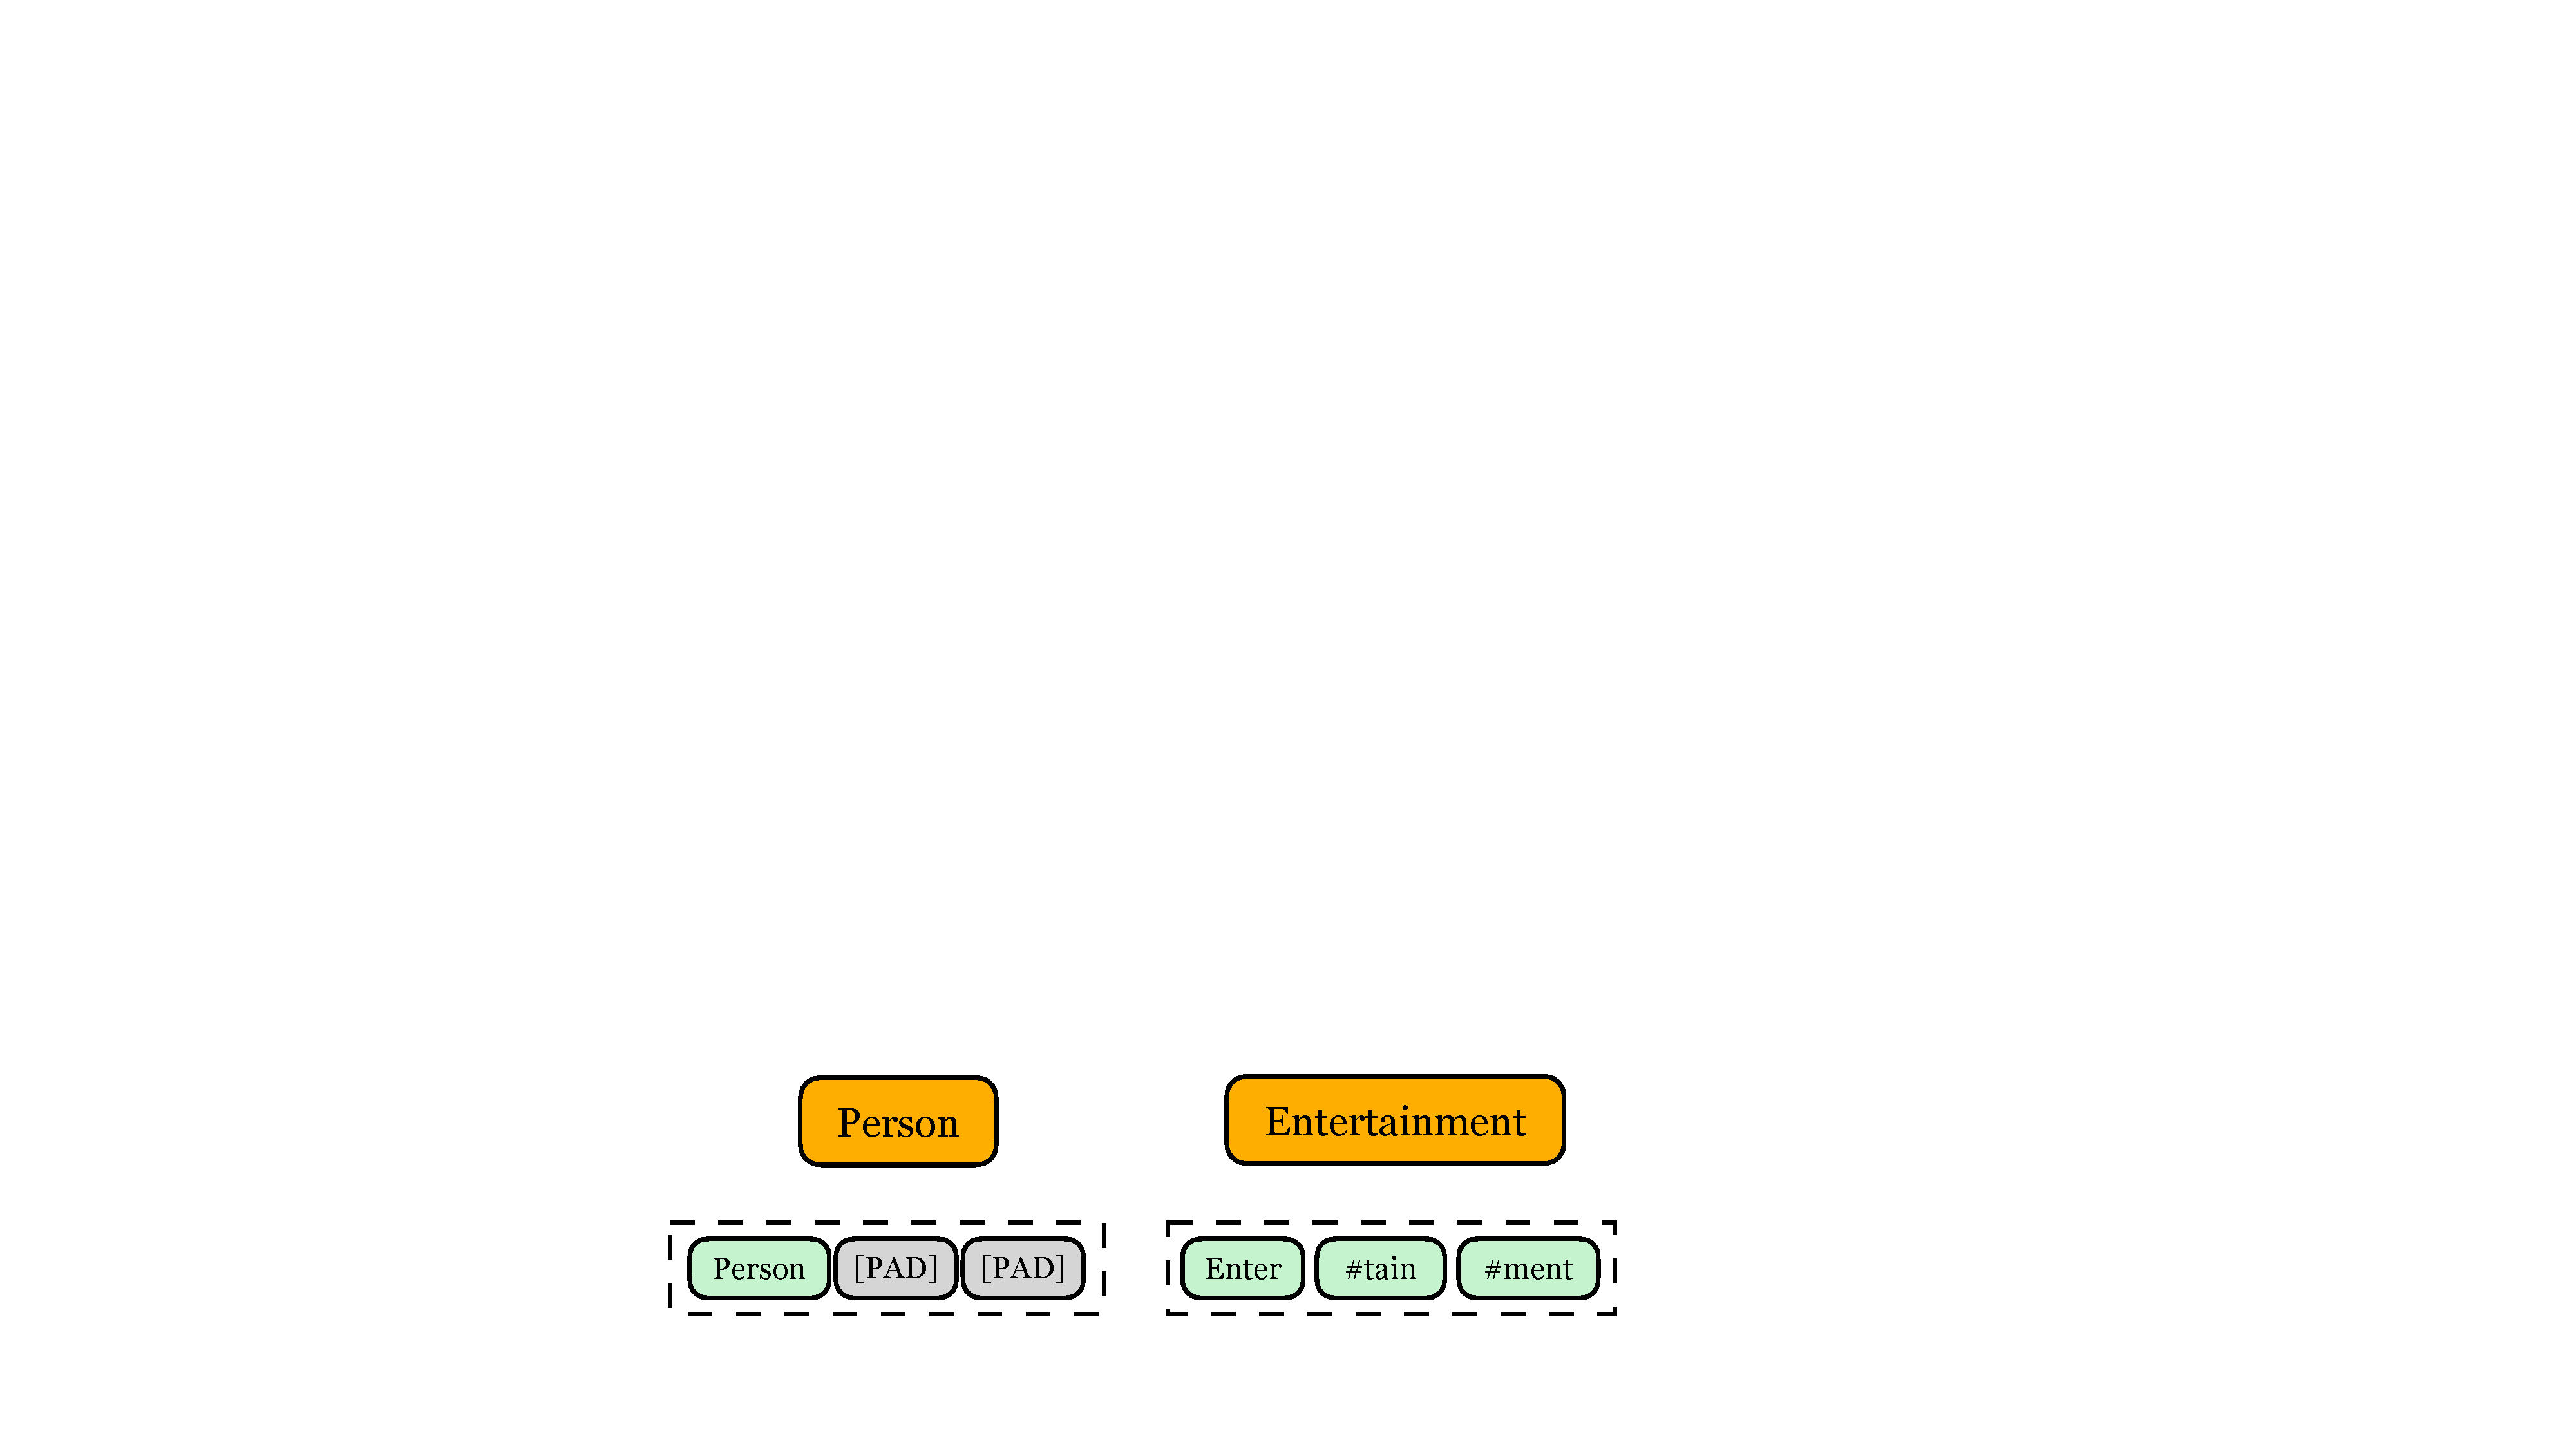
\includegraphics{src/img/cand_block.pdf}}
    \caption{Illustration of candidate block.}
    \label{fig:cand_block}
\end{figure}

\subsection{Attentions in \name}
\label{sec:attn}
There are four kinds of attention in {\bf \textsc{\name}} as shown in Figure \ref{fig:attn1}, sentence to sentence (S2S), sentence to candidates (S2C), candidate to sentence (C2S), and candidate to candidate (C2C). As we score candidates based on mention and its context, attention from candidates to the sentence (C2S) is necessary. However, the necessity of C2C, S2S, and S2C is questionable. As our analytical experiment in Sec. \ref{sec:analyze} shows, it is important for words in the sentence to attend to all candidates (S2C), and is useful to have self-attention in the sentence (S2S), but the attentions (C2C) between different candidates are unnecessary. Based on these findings, we propose a new variant of {\bf \textsc{\name}} that the C2C attention is discarded in computation as shown in the right part of Figure \ref{fig:attn1}. Let $L_S$ and $L_C$ be the number of sub-tokens used by the sentence and candidates respectively. We can formulate the attention query of the sentence as $\bm{Q}_S=[\bm{q}^s_{1};\cdots;\bm{q}^s_{L_S}] \in \mathbb{R}^{L_S \times D}$,  where $\bm{q}^s_i$ is the query vector of the $i$-th sub-token in the sentence, and $D$ is the embedding dimension. Similarly, the query of candidates is formulated as $\bm{Q}_C=[\bm{q}^c_{1};\cdots;\bm{q}^c_{L_C}] \in \mathbb{R}^{L_C \times D}$. When we treat candidates as average of sub-tokens, $\bm{q}^c_i$ is a $D$-dimensional vector, and when we use fixed-sized blocks to place candidates, $\bm{q}^c_i \in \mathbb{R}^{B \times D}$ is the concatenation of the query vectors in the $i$-th candidate block and $B$ is the number of sub-tokens in a block. The keys and values are defined similarly as $\bm{K}_C, \bm{V}_C, \bm{O}_C \in \mathbb{R}^{L_C \times D},  \bm{K}_S, \bm{V}_S, \bm{O}_S \in \mathbb{R}^{L_S \times D}$. The attention outputs are computed as:
\begin{align}
& \bm{O}_S  = \text{Softmax} \big( \frac{\bm{Q}_S [\bm{K}_S; \bm{K}_C]^T}{\sqrt{D}} \big) \cdot [\bm{V}_S; \bm{V}_C] \\
&[\bm{A}_{CS}; \bm{A}_{CC}]  = \text{Softmax} \big( \frac{[\bm{Q}_C \bm{K}_S^T; \bm{M}_C^T]}{\sqrt{D}} \big)  \\
&\bm{M}_C  =  [{\bm{q}_1^c}^T \bm{k}_1^c; \cdots; {\bm{q}_{L_C}^c}^T \bm{k}_{L_C}^c] \\
&\bm{A}_{CC} = [\bm{a}^c_{1}; \cdots; \bm{a}^c_{L_C}] \\
&\bm{O}_C = \bm{A}_{CS} \bm{V}_S + \sum_{j=1}^{L_C} \bm{a}_j \bm{v}^c_j
\end{align}
where $\bm{A}_{CC}$ is the intra-candidate or intra-block attention, and $\bm{a}_j^c$ is a scaler when we treat candidates as average of sub-tokens and is a $B \times B$ matrix when we represent candidates as blocks. The last step (Eq. 8) can be parallelly implemented by Einstein summation.
In most cases, candidate length $L_C$ is significantly larger than sentence length $L_S$. As a result, by ignoring the C2C attention, the inference speed is further improved because the time complexity of the attention is significantly reduced from $O(D(L_S+L_C)^2)$ to $O(D(L_S^2+2L_SL_C+B^2L_C))$. More importantly, the space complexity in attention also gets reduced from $O((L_S+L_C)^2)$ to $O(L_S^2+2L_SL_C))$, which allows us to filter more candidates concurrently. The improvement in space and time complexity by discarding C2C attention is more obvious when the number of candidates becomes larger.

\begin{figure}[h]
    \centering
    \scalebox{0.22}{
    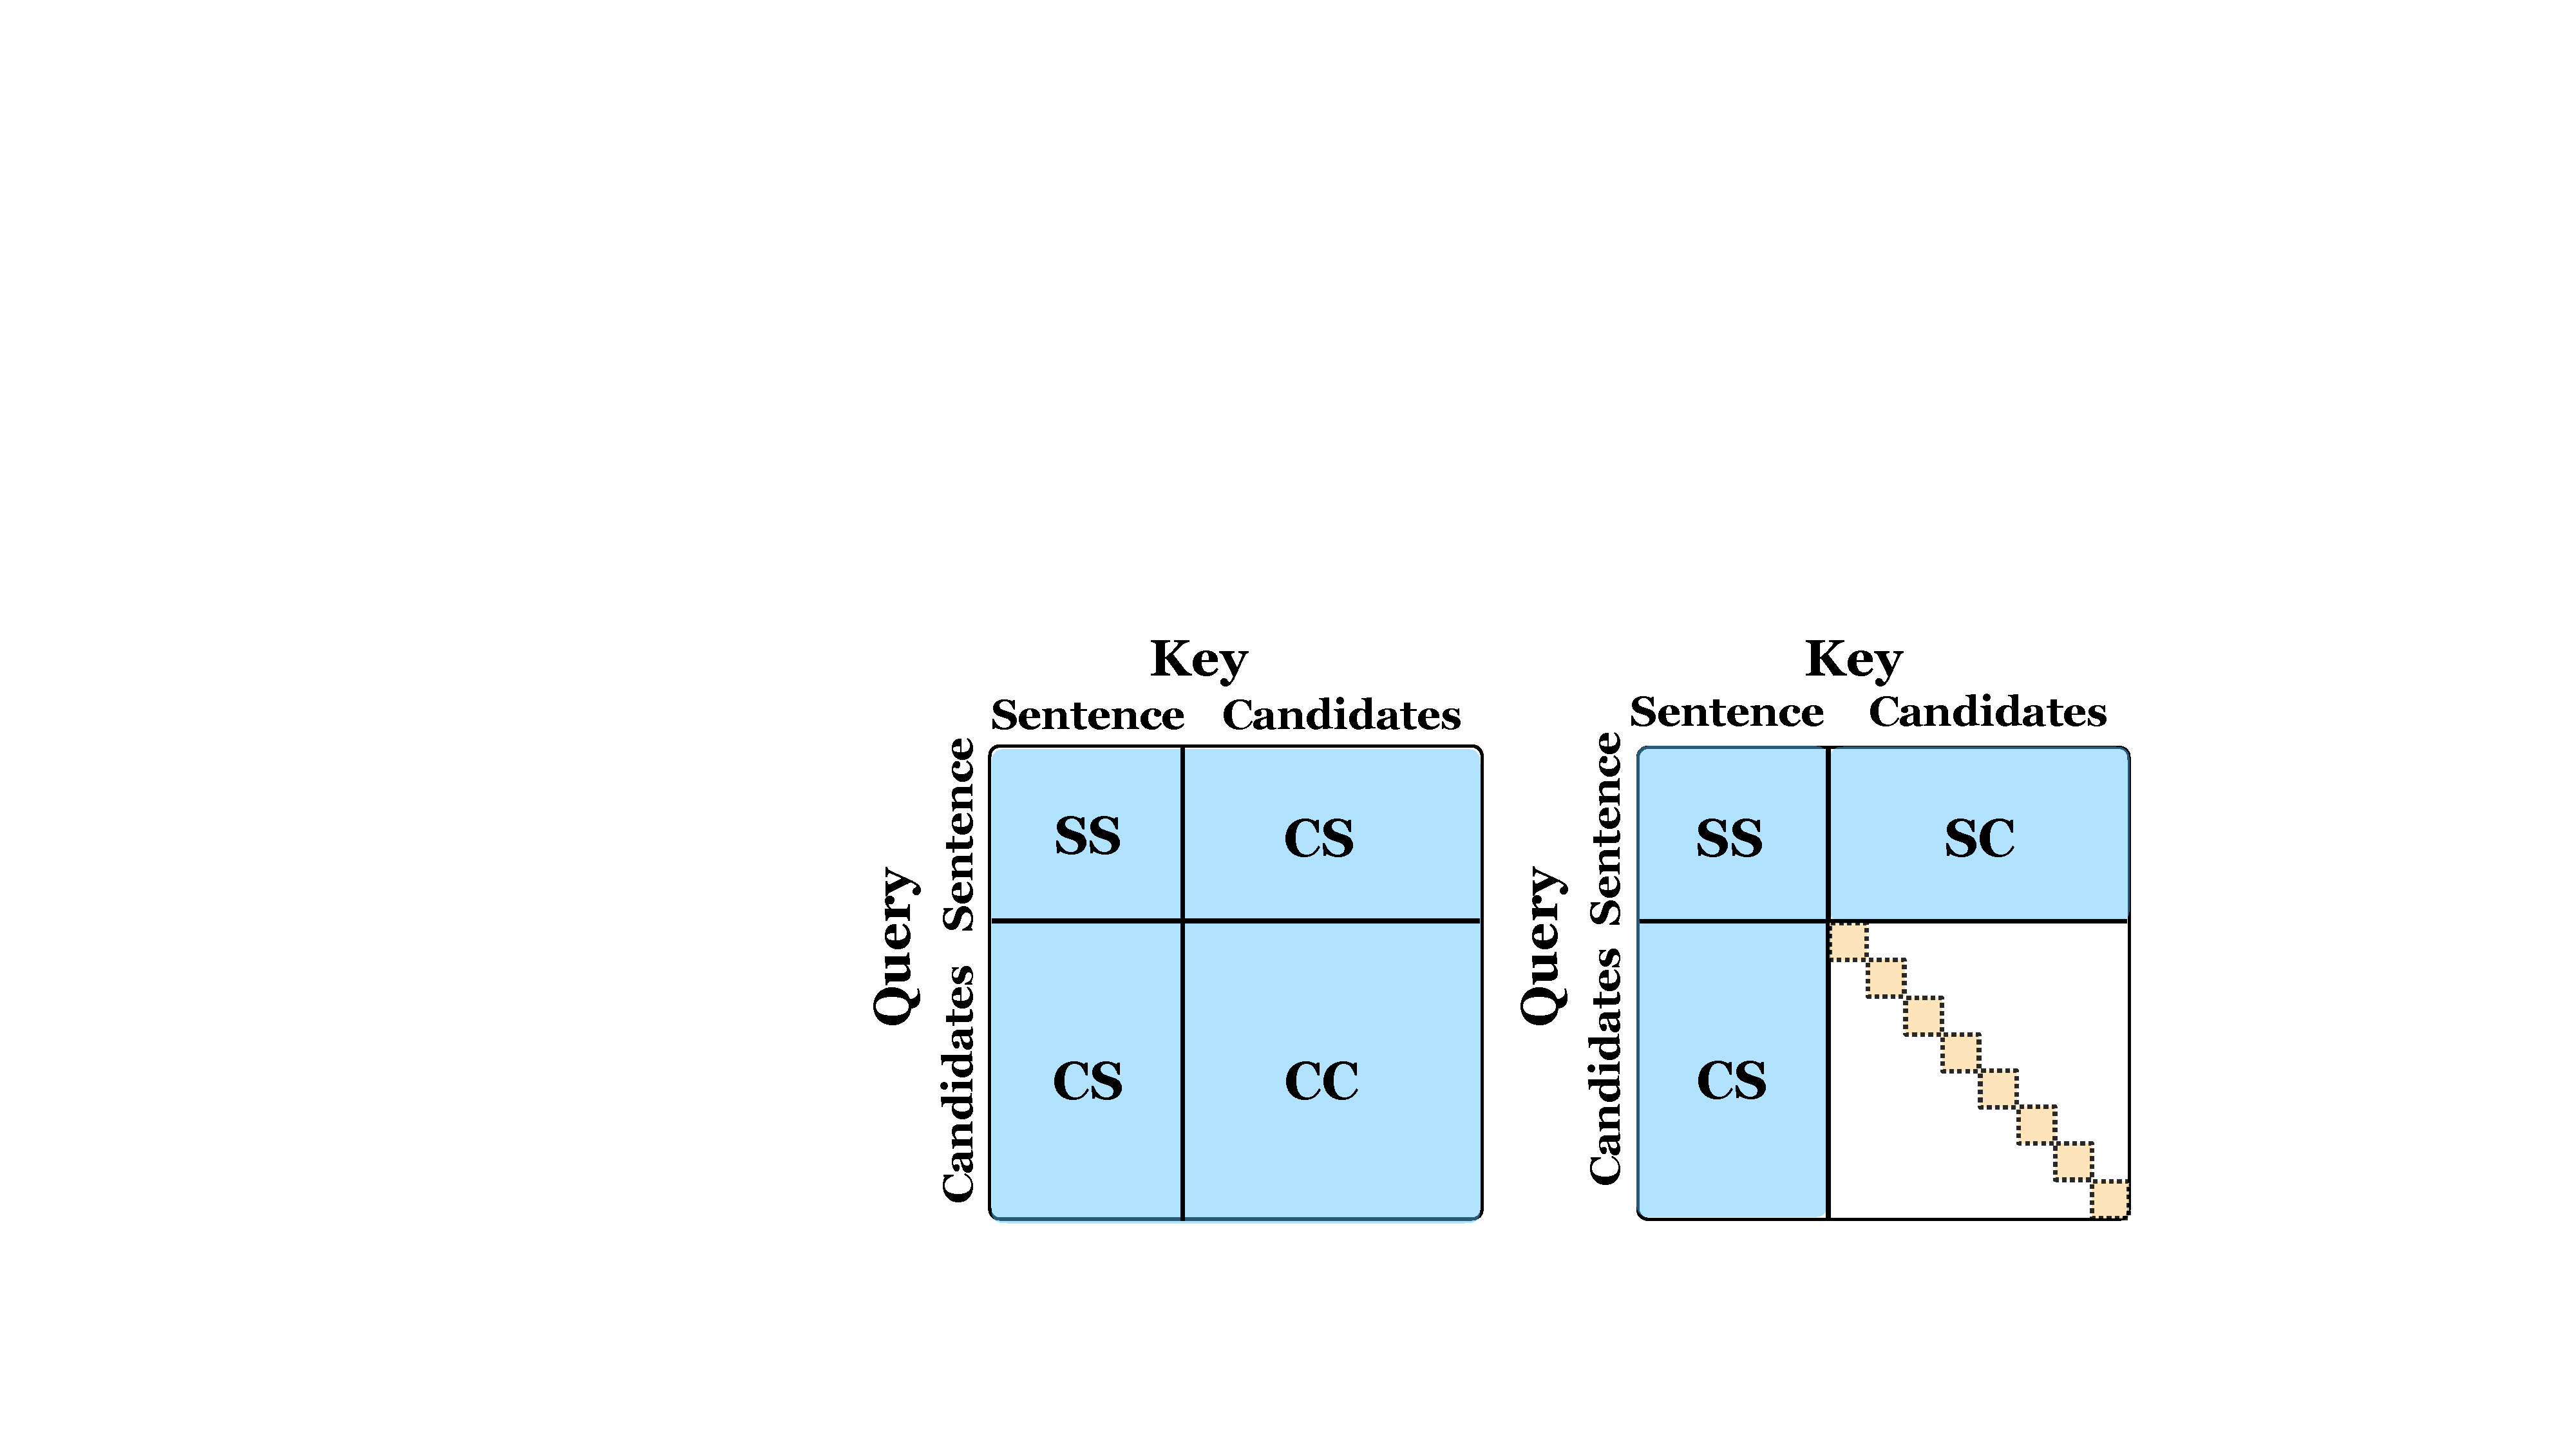
\includegraphics{src/img/attn_all.pdf}}
    \caption{Attentions in {\bf \textsc{\name}} (left), and {\bf \textsc{\name}}  without candidate-to-candidate (C2C) attention (right).}
    \label{fig:attn1}
\end{figure}
\section{Bootstrap Sampling Reddit Comments for Analysis}
Having established the process for identifying macro norm violating comments on Reddit, we proceeded to apply this process to study the prevalence and characteristics of such comments. Our core strategy for doing this was to take random samples of the online comments from our study subreddits, calculating the classifier agreement scores for each of the samples’ elements, and then taking random samples from those comments that were flagged as potentially norm violating (classifier agreement $\geq 80$). But this effectively meant that we were sampling from different subsets of the population in which some of our random samples have a lower rate of violating comments than others due to the differences in the rate of violating comments between different subreddits. 

This makes drawing conclusions from our samples using the traditional inferential statistics problematic---we cannot simply calculate a binomial proportion confidence interval, because we have several convolved sources of uncertainty. The most straightforward parametric statistical procedure would be to select random comments, label them as violating or not violating, and estimate overall levels of violation from that. Unfortunately, due to the large class imbalance (most comments are not violating), this procedure is not tractable. Our introduction of the machine learning layer to nominate possible violations helps manage this problem, but threatens the random sampling procedure and can make errors itself. So, ultimately, we chose to use the classifiers to identify (noisily) a proportion of comments that are violating, complemented with human labeling at a smaller scale to verify. This means that our sampling procedure compounds multiple types of uncertainty: which comments are sampled from the dataset, which comments are flagged by the classifiers, and which comments are verified as actually violating by human annotators.

Given this, we applied a statistical \textit{bootstrapping} technique, variations of which have been used in prior work with similar compounded uncertainty, to derive an accurate measurement and confidence intervals. The core purpose of bootstrapping is to draw conclusions about a population by resampling with replacement from the sample data, which allows for direct observation of the sampling distribution of statistics of interest \cite{61_Varian, 62_Weisstein}. We used the results from our bootstrapping to estimate our key statistics and provide their confidence intervals. 

\begin{figure}[tb]
  \centering
  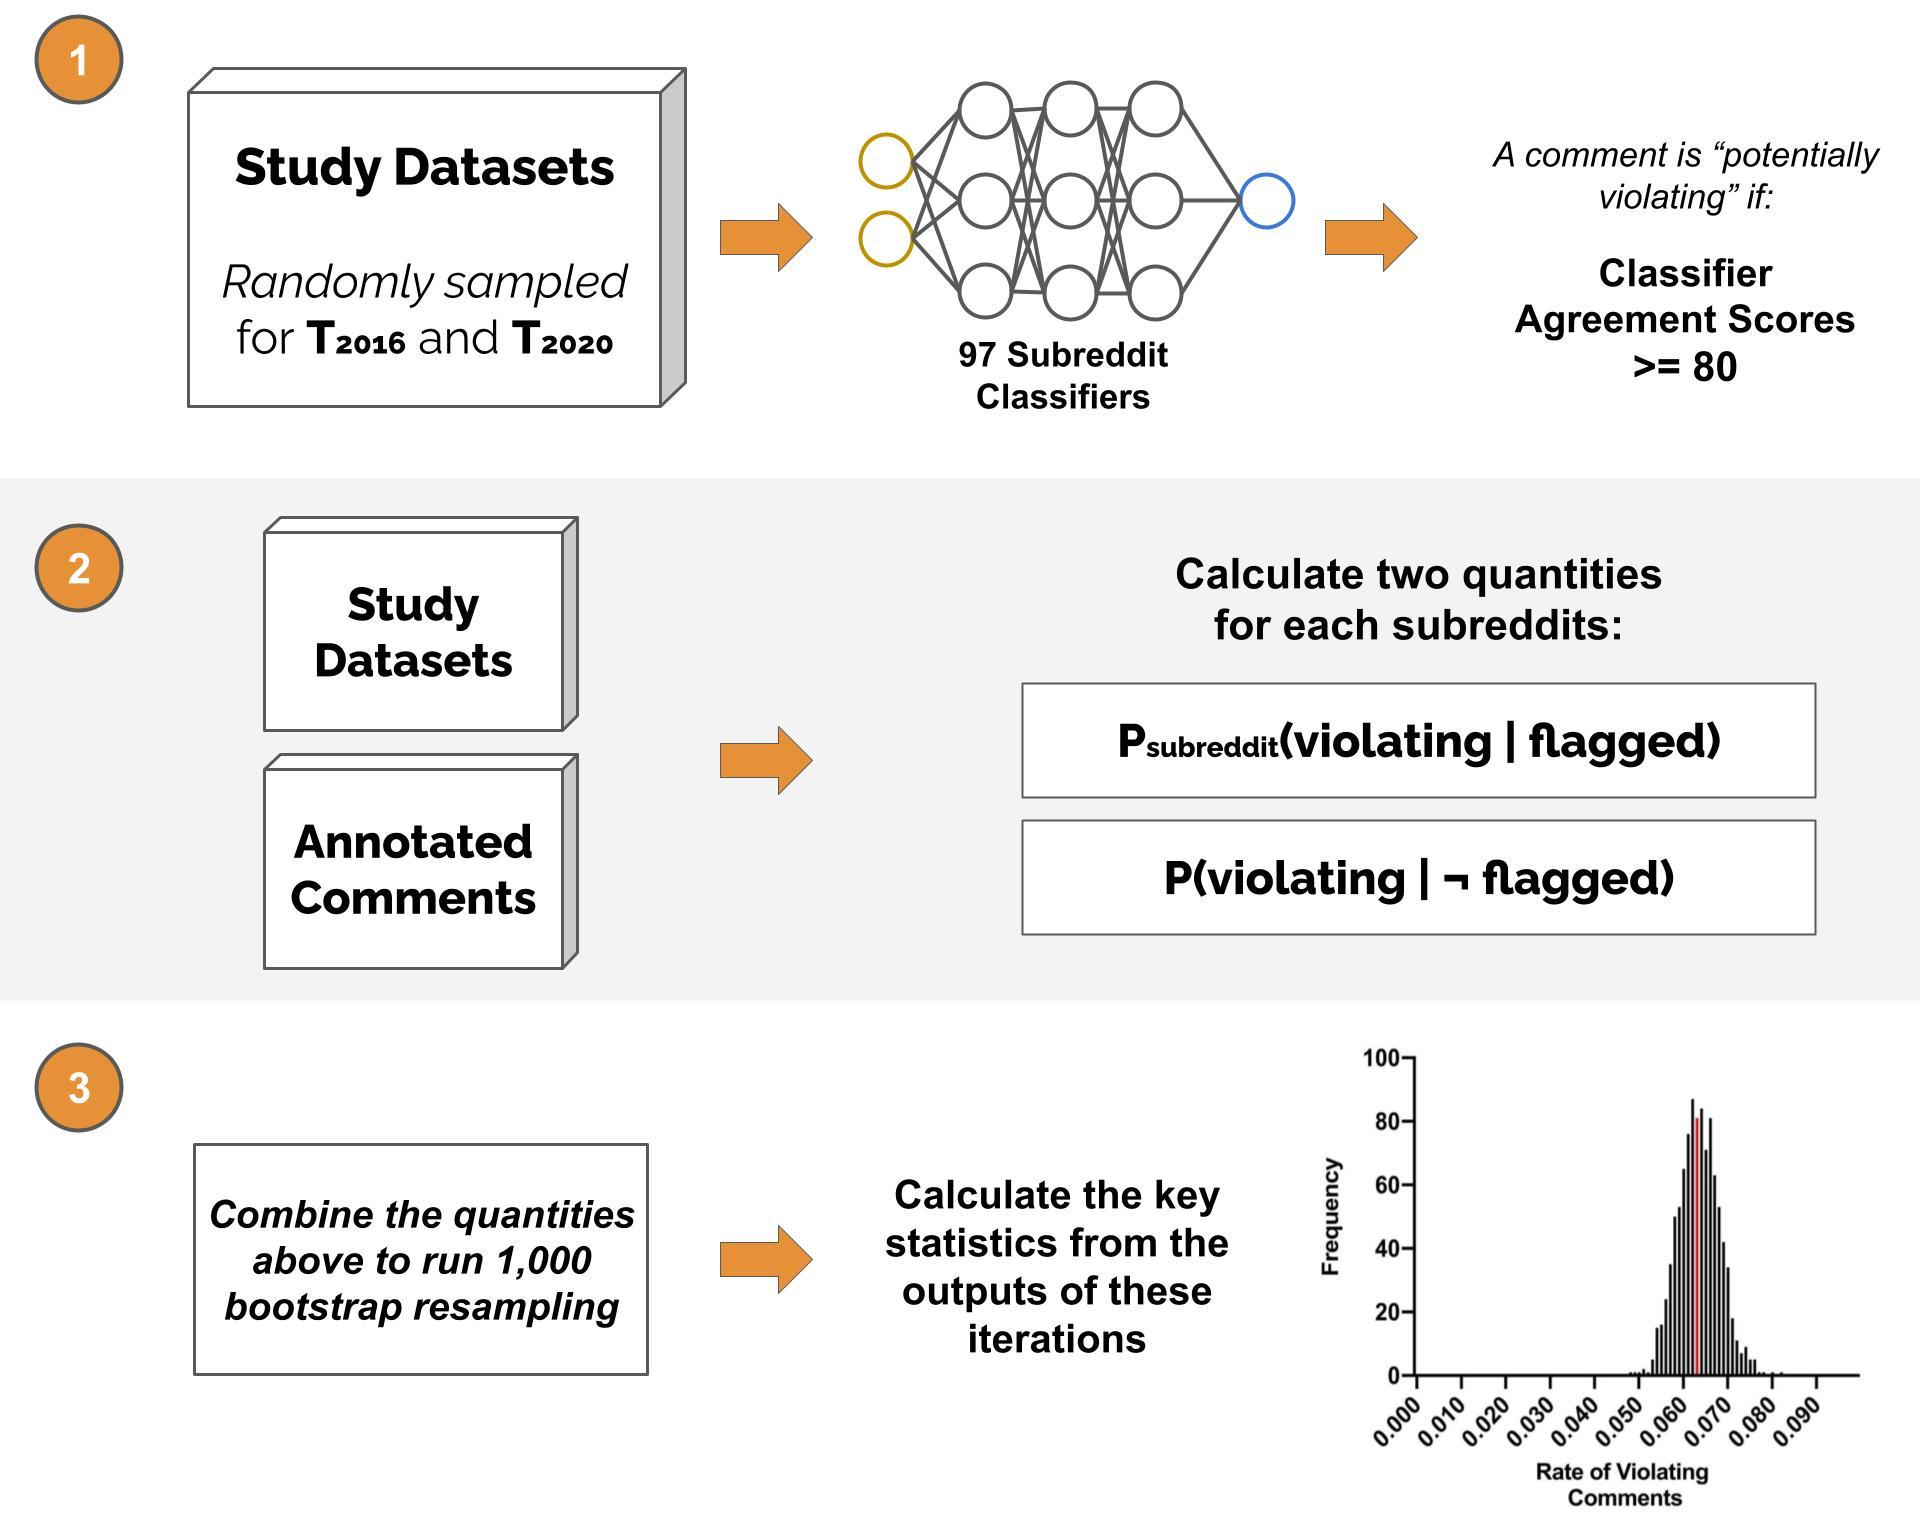
\includegraphics[width=1.0\textwidth]{content_minor_revision__Apr2022/images/bootstrap_workflow_6.jpg}
  \caption{\rnr{An overview of the sampling process in broad strokes. We start by randomly sampling unmoderated comments from $T_{2016}$ and $T_{2020}$ to generate our study datasets. We use these datasets and the annotated comments to calculate key quantities needed for our bootstrap resampling. We then combine these quantities to implement our resampling procedure, which we repeat 1,000 times for each time periods of our interest.}}
  \label{fig:bootstrap}
  \Description{Bootstrap resampling workflow}
\end{figure}


\subsection{\rnr{Bootstrapping Resampling Process}}
We took the following steps to sample our data for bootstrapping. For simplicity, we will describe our method with reference to the May 2016--March 2017 dataset, which we will refer to as $T_{2016}$. 

Intuitively, a bootstrap uses resampling with replacement to create a large number of parallel universes, each with the same number of comments as the original dataset, but each universe will have a slightly different number of norm violating comments due to the resampling with replacement. This variation across many parallel universes is what yields uncertainty confidence intervals on our estimates. However, each universe (bootstrap sample) must also contend with the fact that we have not manually annotated all 5 million comments in the dataset as violating or not. Rather than use a single fixed measurement of norm-violating comments per subreddit, which would ignore this source of uncertainty in the estimation, we resample our annotations over and over again with replacement to build in uncertainty due to our limited number of annotations. Figure~\ref{fig:bootstrap} provides an overview of this process, which is explained in detail below.

\subsubsection{\rnr{Study data and the flagged comments}} 
We began by randomly sampling a set of unmoderated comments. Specifically, we sampled 5,000 random comments from each of the study subreddits posted during this period dataset, for a total of 485,000 comments. These comments were sampled from the Pushshift Reddit corpus, which contains a complete capture of all comments on each subreddit. For clarity in presentation, we will call this sample of comments from 2016--2017, $T_{2016}$. We then ran all 97 subreddit classifiers on each of the sampled comments to calculate the classifier agreement score. Any comments that were flagged by at least 80 of the 97 classifiers as violating were labeled as \textit{flagged}.

\subsubsection{\rnr{Calculating intermediate probabilities}}
For the bootstrap, we needed to follow a procedure where we sample a comment, label it as flagged or not based on the classifiers, and then label flagged comments as violating or not based on human annotators. However, because we cannot tractably label every flagged comment in the bootstrap via human annotation, we relied on statistical generalization via the bootstrap. For this generalization to succeed, we require two empirically observed probabilities for each bootstrap iteration: $P_{subreddit}(violating \mid flagged)$, the true positive rate, the probability that a flagged comment in a particular subreddit is verified by annotators as an actual violation; $P(violating \mid \lnot flagged)$, the false negative rate, the probability that a comment that is not flagged as potentially violating via our classifiers is in fact violating according to our annotators.

\paragraph{$P_{subreddit}(violating \mid flagged)$.} The true positive rate, $P_{subreddit}(violating \mid flagged)$, carries uncertainty since we can only manually annotate a fixed number of comments per subreddit. To model this uncertainty, we re-estimate $P_{subreddit}(violating \mid flagged)$ with each bootstrap resample. Each iteration, for each subreddit, we take a random resample with replacement of the 32 flagged comments that annotators had labeled for each subreddit with each resample (e.g., sample 32 comments with replacement from the set of 32 flagged comments for the subreddit). This value of $P_{subreddit}(violating \mid flagged)$ is then used for that subreddit for that bootstrap iteration and varies with each iteration, capturing uncertainty in our estimate, and is used to help estimate whether a flagged comment in our sample is a true positive.

\paragraph{$P(violating \mid \lnot flagged)$.} Some comments that the classifiers do not believe to be macro norm violations will, in fact, be violations---and our bootstrap procedure must account for this so that it does not undercount the number of violations. To estimate the false negative rate, $P(violating \mid \lnot flagged)$, we use the sample of 1,000 \textit{non-flagged} unmoderated comments that we manually annotated in Section 3.4. These 1,000 comments showed a consistent 1\% false negative rate of our classifiers across 10 randomly chosen subreddits, so we treat this value as being consistent across all subreddits and do not parameterize it by subreddit. However, we still must model uncertainty in this estimate. So, for each bootstrap iteration, we resample 1,000 comments with replacement from the set of 1,000 comments and calculate $P(violating \mid \lnot flagged)$ as the proportion of comments that were not flagged as potentially violating but were in fact violating according to human annotators. We use this quantity to estimate whether a non-flagged comment in our sample is a false negative. As with the true positive rate, resampling with replacement will cause this value to vary from bootstrap iteration to iteration, critical to creating confidence intervals for our analysis.

\subsubsection{\rnr{Bootstrap resampling iteration procedure}}
These two probabilities enable our bootstrap procedure. In bootstrapping, we resample the dataset many times and measure the quantity of interest in each new instance. \rnr{In this study, we ran our bootstrapping procedure for 1,000 iterations (this is a typical number of iterations when conducting bootstrap resampling \cite{81_Bootstrap}). For each iteration, we resampled a number of comments that matched the complete number of comments on each of our study subreddits during our study period (i.e., 252,642,908 comments for $T_{2016}$). We also resample with replacement from the dataset of 5,000 classified comments each iteration, creating variation to model uncertainty in our sampling. Each bootstrap iteration also estimates new values for $P_{subreddit}(violating \mid flagged)$ and $P(violating \mid \lnot flagged)$ for each iteration, which combine to provide one datapoint in the final outcome distribution. In other words, each bootstrap sample creates an alternative universe of comments resampled from each subreddit, exhibiting natural variation in violation and moderation rates due to the random sampling.}

We illustrate this process with an example of bootstrap resampling the r/videos subreddit for $T_{2016}$. There were a total of 5,296,900 unmoderated comments that were on r/videos during $T_{2016}$. To populate each of these comments, we sampled a random comment from the subset of 5,000 random comments from r/videos that the classifiers had labeled. These 5,000 random comments had themselves been randomly sampled with replacement for this iteration of the bootstrap from the original set of 5,000 comments that were collected and classified. For r/videos, in one of the bootstrap samples, 1,249 of the 5,000 randomly sampled unmoderated comments (25\%) were flagged as potentially violating by the classifiers. If the sampled comment was flagged, then we randomly assign the comment as violating with probability $P_{r/videos}(violating \mid flagged)$ ($\approx 0.2$ in this bootstrap iteration) and attach the violation type(s) that human annotators tagged that comment with, and as not violating otherwise. If the sampled comment was not flagged, then we randomly assign the comment as violating with $P(violating \mid \lnot flagged)$ ($\approx 0.01$ in this iteration), and not violating otherwise. This process repeats to generate all 5,296,900 comments for r/videos.

We follow this process for all 97 subreddits, for all 1,000 bootstrap samples. The 1,000 samples provide a distribution and uncertainty estimate for the key statistics. Finally, through this process, we resample the same number of comments as the number of all unmoderated comments that were posted on these subreddits, some of which are labeled to be violating. So when we calculate the rate of unmoderated but violating comments in one bootstrap iteration, we add up the number of unmoderated but violating comments in each of the 97 subreddits and divide that by the number of all comments --- this gave us an estimation for r/videos, which was 5.95\% [2.16, 9.22] for $T_{2016}$, and 3.53\% [0.59, 9.14] for $T_{2020}$. This allows our bootstrap procedure to naturally take into account the different subreddit sizes --- through resampling more comments from the larger subreddits, the bootstrap will give more weight to the uncertainty on larger subreddits, in the analysis which are focused on the overall rates across the platform.

\subsubsection{2020 dataset}
As mentioned in the previous section, there are two periods of interest: one, from May 2016 to March 2017, the same period as when the moderated comments dataset $\mathcal{M}$ was collected, and the other from the last three weeks of December 2020, which we consider as a replication study on a slightly shorter but more recent timeframe. As we referred to the original dataset as $T_{2016}$, we will refer to the latter as $T_{2020}$. The process for $T_{2020}$ was identical to $T_{2016}$. Because $T_{2020}$ was a smaller dataset, however, its constituent samples were fewer in number. In particular, we \rnr{randomly} sampled 2,000 comments from each of the study subreddits instead of 5,000 commments, or fewer if the subreddit did not contain 2,000 comments during $T_{2020}$. This resulted in a total of 188,000 comments sampled and run through our 97 subreddit classifiers. Given the smaller sample size, the confidence intervals are wider for $T_{2020}$ than for $T_{2016}$.

\subsection{\rnr{Ablation Analysis with Fewer Annotations}}
Our bootstrap relies on a set of thousands of manually annotated comments from annotators. This gives rise to a possible threat to validity: that we did not manually annotate enough comments per subreddit to capture the uncertainty in the estimate per subreddit. To test whether this threat should be concerning, we performed an ablation analysis where we replicated our method using half of the manual annotations we had for each of the subreddits (that is, 16 annotations per subreddit instead of 32 for $T_{2016}$, and 4 per subreddit instead of 8 for $T_{2020}$). The main goal of this ablation analysis was to test how having fewer annotations impacts the uncertainty estimates of the bootstrap. Intuitively, as we have fewer and fewer samples, the confidence intervals will widen because if a rare event is sampled, it has a larger impact on the resulting estimate. We report our findings alongside our main results, in Section 6.

\section{Measurements}
Using our pipeline for identifying violating comments and bootstrap sampling of comments, we estimated the dependent variables of interest. In this section, we present our specific measures that we derived from our method. 


\subsection{Estimating the Prevalence of Violating Comments}

\subsubsection{Overall prevalence} 
Our core dependent variable is the percentage of unmoderated comments that are \rnr{macro norm} violations. For each bootstrap sample, we calculated the percentage of violating comments. We then calculated our estimate as the median result across the 1,000 bootstrap samples, and calculated the 95\% confidence interval across those samples. 

\subsubsection{Prevalence per subreddit} 
Do some subreddits contain a higher rate of macro norm violating comments than the others, and if so, why? To answer this question, we estimated the percentage of violating comments for each of the subreddits across each of the bootstrap samples, and again calculated the median and 95\% confidence interval per subreddit. Given that the $T_{2020}$ sample, as mentioned previously, is a smaller scale replication of the $T_{2016}$ sample, we found that there is not enough data to draw statistically meaningful results for each of the subreddits for $T_{2020}$. Therefore, we focused our analysis in this particular subsection on the $T_{2016}$ sample. 

We tested the factors that were associated with a subreddit having a higher count of violations. We started by taking the sampling approach as we did above to estimate the count of violating comments for each of the study subreddits. We hypothesized that two relevant predictive variables might influence the rate of violating comments: 1) the topic of a given subreddit and 2) the ratio of the number of moderators to the number of comments. Our focus on the first variable was motivated by our observation that some communities might be more prone to hosting macro norm violations that are topically relevant (e.g., politically inflammatory comments for political subreddits or pornography for NSFW subreddits), while our focus on the second variable was informed by prior work suggesting that moderators in subreddit communities are overloaded and unable to review every comment posted~\cite{Chandrasekharan2018internet, 18_Gilbert}.

To test these hypotheses, we first collected the relevant data for these variables. To get the respective topics for our study subreddits, we matched the study subreddits to categories on r/ListOfSubreddits’ thematically organized list of subreddits.\footnote{\url{https://www.reddit.com/r/ListOfSubreddits/wiki/listofsubreddits}} The list contains multiple layers of thematic hierarchy. From this, we picked the second-highest thematic layer (e.g. r/AskReddit was categorized as “Discussion,” and r/Pokemon as “Entertainment”) for our subreddits as the top layer was too broad to be meaningful. This resulted in eleven mutually exclusive topic categories for our 97 study subreddits.  We then manually collected the number of moderators who were present in October 2016 (the middle of the 11-month period when $\mathcal{M}$ was collected) for each of the subreddits by using the Wayback Machine to access an archived version of each subreddit's homepage on October 1st, 2016, or the earliest subsequent date when the page was crawled. We then calculated the ratio of moderators to comments for each of the subreddits. Finally, we retrieved the number of all comments (including those that were removed by the users or moderators) that were posted on each of the 97 study subreddits from $T_{2016}$ -- we used this information as the offset to our Poisson model described below. To address the non-normal distribution of the number of comments and moderator-to-comment ratio in our regression, we log transformed these variables.

We then employed a Poisson regression \cite{63_poisson} to model the rate of macro norm violating comments in a given subreddit using the three aforementioned predictive variables as our independent variables. \rnr{Poisson regression was an appropriate choice because it is designed to model rate data. We followed a common practice of setting an offset---in our case, the size of the subreddit in terms of the number of comments--- to the Poisson regression model to make it appropriate for rate data \cite{94_Anderson, 95_Gardner}.} For better interpretability of our model, we treated the ``general content'' topic category as the baseline of the indicator (dummy) variable for topic. Finally, to interpret our results, we exponentiated the variable coefficients in our model to calculate the incidence rate ratios. For instance, as we will cover in the next section, \rnr{the number of moderators to comments ratio in a subreddit is a significant predictor of the rate of violating comments in a subreddit (p<0.001) where for every unit increase in the log-transformed number of comments in a subreddit, the rate of violating comments is expected to increase by a factor of 2.07 (=$e^{0.728}$).}


\subsection{Determining the Characteristics of Violating Comments}

\subsubsection{Prevalence by violation category} 
So far, we defined a comment to be violating if it violates one of the macro norms of Reddit. But here, we describe our analysis that takes a closer look at the variance in the prevalence of different macro norm violations and the rate at which they occur. In order to better understand the prevalence of each of the macro norm violations among the unmoderated comments, \rnr{we measure the percentage of sampled violations that fall into each of the violation categories}. Specifically, we take the average number of norm violations per category that across the study subreddits in each bootstrap iteration, and as before, report the median and confidence interval across the 1,000 bootstrap iterations.

Are all categories of macro norm violations removed by the moderators at the same rate? To answer this question, we \rnr{take the following steps to} estimate the number of all comments (moderated and those still online) that violate each specific one of the macro norms. To estimate the number of violations for each of the macro norms within the moderated comments, we require a complete set of all moderated comments from our study subreddits, which we gathered earlier as $\mathcal{M}$ for $T_{2016}$. To extend $\mathcal{M}$ to $T_{2020}$, we reimplemented the original high-frequency scraping process used in prior work to generate $\mathcal{M}$ for $T_{2016}$~\cite{Chandrasekharan2018internet}. We then randomly sampled from $\mathcal{M}$ (N=776 comments for the longer $T_{2016}$ period; N=188 for the shorter $T_{2020}$ period). We then followed the same human annotation process from Section~\ref{sec:annotation} to annotate each moderated comment with any macro norms that it violated. Using this, we calculated the estimated number of comments that violate each of the macro norms within the moderated comments dataset. We combined this with the estimated number of unmoderated violations for each macro norm to estimate the overall number of violations for each of the macro norms considering both moderated and unmoderated comments combined. With this number of violations, we then proceeded to calculate the rate at which each of the macro norms are moderated.

\subsubsection{Comparing the rate of engagement} 
Reddit comments accrue engagement over time in the form of upvotes, downvotes, and replies. The “score” of a comment is determined by subtracting the number of downvotes from the number of upvotes the comment gained over time, and “replies” are comments that respond to the given comment in the thread. Score is a useful dependent variable to track because it is a strong determinant of how high in the thread the comment sits.\footnote {On Reddit, users can choose one of the three options -- top, hot, and best -- for determining what comments should come at the top. Top is simply whichever comment has the highest score, hot is the log-transformed absolute value of the score with extra weights for the age of the content, and best is the number of upvotes divided by the number of downvotes. See \url{https://www.reddit.com/r/explainlikeimfive/comments/1u0q4s/eli5_difference_between_best_hot_and_top_on_reddit/}} The number of top-level replies can serve as a proxy for measuring whether the given comment generated, or ended, a discussion.\footnote{The Perspective model from Jigsaw for measuring toxicity used human annotations to train where a comment was asked to be annotated if it were “rude, disrespectful, or unreasonable… that is likely to make you leave a discussion” \cite{60_Perspective}.}
We explored whether the violating comments result in significantly higher or lower scores, and whether they receive more or fewer “top-level replies” (replies that directly respond to the given comment in the thread of replies). To investigate this, we compared the scores and the number of top-level replies that the unmoderated violating comments got to the global average number of online comments the study subreddits in our $T_{2016}$ and $T_{2020}$ samples.


\subsubsection{Comparing language usage} 
Does the way in which a macro norm is violated impact its likelihood of remaining on the site or being moderated? We compared the writing style of moderated comments vs. unmoderated violating comments on two dimensions: readability and emotionality. For measuring readability of a comment, we used the Flesch–Kincaid readability test~\cite{64-kinkaid} to retrieve the comment’s readability score, where a higher score indicates that the comment is easier to read. For measuring emotionality of a comment, we used Evaluative Lexicon 2.0~\cite{65_Rocklage, 66_Rocklage}, an imputation-based dictionary that assigns an emotionality score to text where higher score means that the comment is more likely to trigger an emotional reaction rather than a cognitive response that reflects a person’s beliefs about the topic of discussion \cite{66_Rocklage}.


\section{Results}
\label{ss: results}

In this section, we address the research questions from Section~\ref{ss: questions} 
by applying the methodology from Section~\ref{ss: metrics}.
We apply \nbAnalyzers{} widely used PDF scanners to a total of \nbSamplesSize{} malicious PDF documents generated by the Chameleon framework and an additional \nbBenignsSize{} benign PDF documents.
The benign documents comprise train tickets, governmental documents, manuals, tutorials, and some suspicious looking PDF files that are known to be benign.
All documents used for our study will be made available as a benchmark for future work.

\subsection{RQ1: Recall and False Positives}
\label{ss: recall fps}

The following addresses RQ1, i.e., how accurately the scanners classify 
documents into malicious and benign in the presence of evasions.
We measure the recall and the false positive 
ratio of each scanner, as described in Section~\ref{ss: metrics}.
Figure~\ref{fig: recall fp ratio} shows the results.
A higher recall means that the scanner is more successful in 
identifying malicious PDF documents, despite the presence of evasions.
The figure shows that almost all studied scanners are affected by evasions, 
as their recall values are lower than 100\%.
Furthermore, we find a huge variation across the studied scanners: While 
some scanners, e.g., SAFE-PDF and AVG, identify all or most malicious documents despite 
evasions, others miss many malicious documents.
Some scanners have a recall lower than 20\%, showing that they are easily 
bypassed by evasions.

In principle, a scanner could achieve 100\% recall by labeling each document 
as malicious.
To address this potential problem, Figure~\ref{fig: recall fp ratio} also 
shows the false positive ratio of each scanner.
We find that all scanners have a false positive ratio below 15\%, except Cuckoo (17.5\%), Slayer (28.77\%), and SAFE-PDF (34.57\%).
There is no strong correlation (Pearson correlation coefficient: 36.61\%) between recall and false positive ratio.
We conclude from these results that none of the scanners tries to boost its 
recall at the cost of precision, which seems reasonable as users easily drop 
a tool if they are overwhelmed with spurious warnings.


\begin{figure*}[t]
	\begin{minipage}{0.55\textwidth}
		\hspace{-.6em}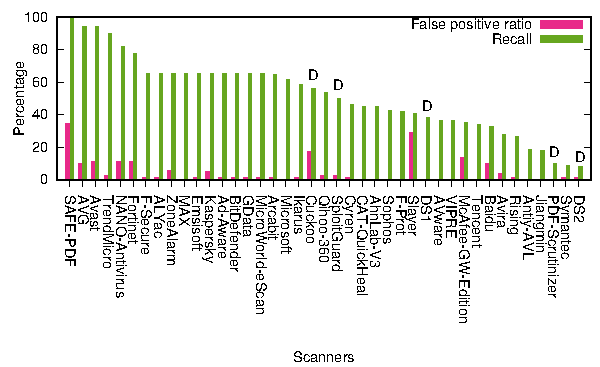
\includegraphics{figures/fp-ratio-recall}
		\captionof{figure}{Recall and false positive ratio of the studied scanners.  
			The dynamic scanners are marked with ``D''.}
		\label{fig: recall fp ratio}
	\end{minipage}
	\hfill
	\begin{minipage}{0.4\textwidth}
		\hspace{-.6em}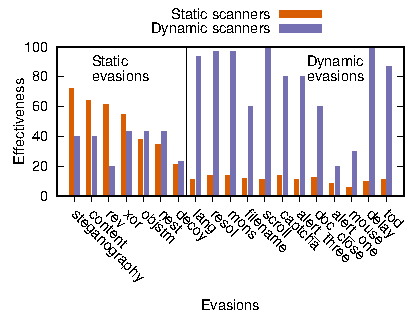
\includegraphics{figures/average-best-case-eff}
		\captionof{figure}{Effectiveness for different classes of static and 
			dynamic evasions. The results are averaged over all static 
			(red) and dynamic (blue) scanners.}
		\label{fig: best case eff}
	\end{minipage}		
\end{figure*}	


\subsection{RQ2: Evasion Effectiveness by Scanner}

To better understand the susceptibility of the scanners to static and dynamic evasions, we assess the effectiveness of evasions in bypassing specific 
scanners (RQ2).
We compute the evasion effectiveness for each 
scanner by averaging the effectiveness across all evasions.
Figures~\ref{fig: static evasions proj} and~\ref{fig: dynamic evasions proj} 
present the results for static and dynamic evasions, respectively.
A lower value indicates that a scanner is less susceptible to evasions.
The results for the static evasions in Figure~\ref{fig: static evasions 
proj} show some interesting effects.
Somewhat surprisingly, the effectiveness of 12 of the~\nbVirusTotalEngines{} VirusTotal scanners, roughly 
in the middle of the figure, is exactly the same, out of which 8 have the exact same recall, too (Figure~\ref{fig: recall fp ratio}).
A possible explanation is that multiple scanners rely on 
the same underlying decision mechanism, e.g., because one scanner queries 
another scanner as part of its decision, or because the same analysis 
algorithm is provided under several brands.
Previous, informal reports claim that some static scanners share their results~\cite{static_analyzers_share_analysis_result}, which our results 
confirm.


\begin{figure*}[tb]
	\begin{minipage}{0.55\textwidth}
		 \begin{subfigure}{\textwidth}
			  	\hspace{-.6em}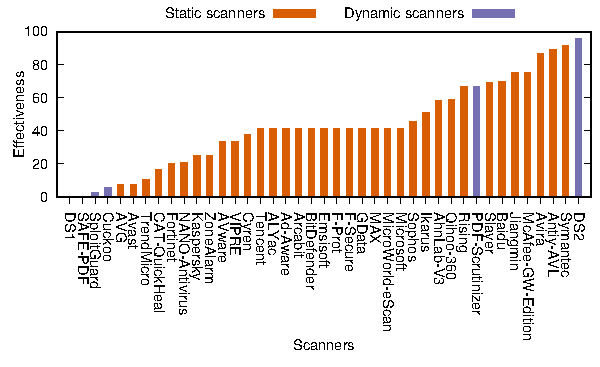
\includegraphics{figures/static-evasions-projection}
			  	\caption{Static evasions}
			  	\label{fig: static evasions proj}
		 \end{subfigure}		 
		 \begin{subfigure}{\textwidth}
			  	\hspace{-.6em}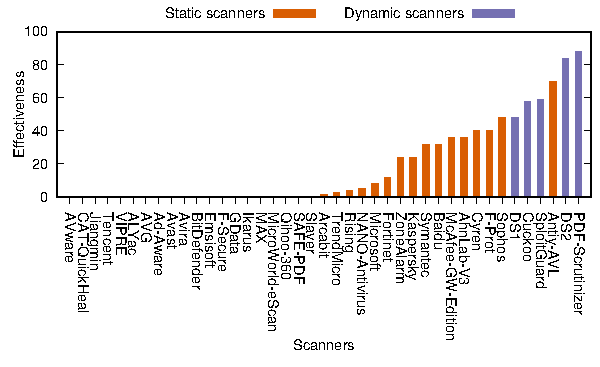
\includegraphics{figures/dynamic-evasions-projection}
			  	\caption{Dynamic evasions}
			  	\label{fig: dynamic evasions proj}
		 \end{subfigure}
		 \caption{Per-scanner effectiveness of static and dynamic evasions.}		
	\end{minipage}
	\hspace{1em}
	\begin{minipage}{0.4\linewidth}
		\begin{subfigure}[b]{\textwidth}
			\hspace*{-.6em}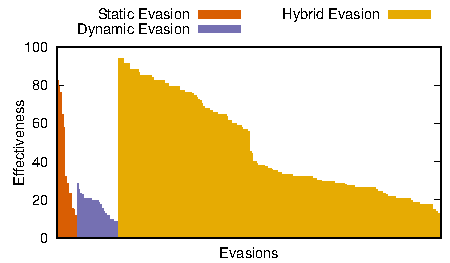
\includegraphics{figures/toolbutton-projection}
			\caption{Documents with ``Toolbutton'' exploit.}
			\label{figure:toolbutton projection}
		\end{subfigure}
		\vspace{2em}
		
		\begin{subfigure}[b]{\textwidth}
			\hspace*{-.6em}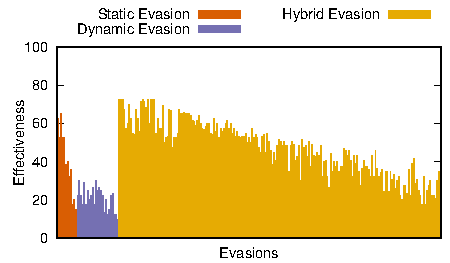
\includegraphics{figures/cooltype-projection}
			\caption{Documents with ``Cooltype'' exploit.}
			\label{figure:cooltype projection}
		\end{subfigure}
		\caption{Effectiveness of evasions for the subsets of malicious documents that use a specific exploit. Each bar corresponds to an evasion with a specific argument. The hybrid evasions, and some of the static and dynamic evasions  result from combining evasions (Section~\ref{ss: combination of evasions}).}
	\end{minipage}
\end{figure*}


Another interesting observation is that a dynamic, not a static, scanner (DS2) is the most susceptible to static evasions.
A comparison of  Figures~\ref{fig: static evasions proj} and~\ref{fig: dynamic evasions proj} shows that DS2 is highly susceptible to both dynamic and static evasions.
This finding suggests that DS2 not only uses dynamic analysis, but also 
heavily relies on static analysis techniques.

The static scanners in the right part of Figure~\ref{fig: dynamic evasions proj} are
impacted by dynamic evasions.
A likely reason is that adding an evasion changes the signature of the PDF documents, and that the scanners rely on these signatures.


\subsection{RQ3: Most Effective Evasions}
\label{ss:best-case effectiveness}

Understanding which evasions are most effective (RQ3) is important both for attackers and for developers of security scanners.
We measure the effectiveness of evasions for each scanner and then compute 
the average over all static and the average over all dynamic 
scanners.
Some evasions take arguments, e.g., the language used by the ``lang'' evasion or the xor key used by the ``xor'' evasion.
For such evasions, we try a range of arguments and report the highest observed effectiveness.

Figure~\ref{fig: best case eff} shows the results.
We sort the evasions as in Table~\ref{t:evasions}.
Overall, the results show that static scanners are much more susceptible to 
static evasions, while dynamic scanners get fooled by dynamic evasions, 
which is unsurprising and confirms our classification of evasions.

Among the static evasions, those related to run-time loading and JavaScript obfuscation are the 
most effective, suggesting that many static scanners rely on checking the 
JavaScript code embedded into PDFs to identify malicious 
behavior.
The high effectiveness of many of the static evasions is somewhat 
surprising given that some of these static evasions have been known 
for several years~\cite{related_static_obfus, corona2014lux0r, more_related_static_obfus}.

For dynamic evasions, attackers can choose from a relatively large set of 
highly effective evasions, including the two time-related evasions, most of 
the context-related evasions, and some of the user interaction-related 
evasions, e.g., ``scroll''.
In contrast, some other UI-related evasions are only moderately effective, e.g., ``mouse''.
The reason is that some of the dynamic scanners use anti-evasion techniques, such as user interaction emulation, to counter these evasions.
For example, Cuckoo moves the mouse after opening a document in a PDF
reader to counter the ``mouse'' evasion~\cite{cuckoo_mouse_movement}.

\begin{table}[]
    \small
    \centering
	\caption{The evasions that bypass all but two scanners. The evasions are applied to a document in the given order.}
	\label{t:detected by two}
    \renewcommand*{\arraystretch}{1.2}
    \setlength{\tabcolsep}{5pt}
    \begin{tabular}{rp{25em}}
    \toprule
    &Combined evasions \\
    \midrule
     1 & mouse, scroll, content, steganography, xor (key: 40) \\
     2 & alert\_one, scroll, content, steganography, xor (key: 40) \\
     3 & alert\_three (trigger on No or Cancel), mouse, mons ($>$1), filename, lang (German), tod (8 AM -- 4 PM), scroll, content, steganography, xor (key: 40) \\
    \bottomrule
    \end{tabular}
\end{table}

To better understand highly effective evasions with their particular arguments across all scanners,
Table~\ref{t:detected by two} lists the evasions that bypass all but two scanners (NANO-Antivirus and SAFE-PDF) for at least one exploit.
All the evasions presented in Table~\ref{t:detected by two} are hybrid, showing that
combinations of static and dynamic evasions are effective as they bypass both static and dynamic scanners at the same time.
Overall, the observation that three different combinations of evasions can circumvent almost all scanners is alarming and motivates future work on anti-evasion techniques.


\subsection{RQ4: Counter-effective Evasions}
\label{ss: Counter-effective Evasions}

In the following we address RQ4, i.e., whether some evasions have the opposite of the expected effect by causing a scanner to detect an otherwise missed malicious document.
To answer the question, we measure the counter-effectiveness of each evasion for each scanner and then compute 
the average over all static scanners and the average over all dynamic 
scanners.
For evasions that take parameters, we report the highest counter-effectiveness observed across a range of values.

\begin{figure}[tb]
    \hspace{-.6em}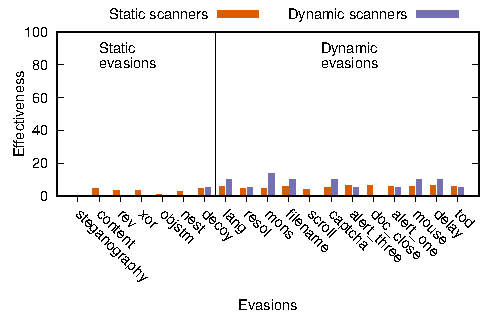
\includegraphics{figures/average-worst-case-counter-eff}
    \caption{Counter-effectiveness for different classes of static and 
    dynamic evasions. The results are averaged over all static
    (red) and dynamic (blue) scanners.}
    \label{fig: worst case counter-eff}
\end{figure}

Figure~\ref{fig: worst case counter-eff} shows the counter-effectiveness of the studied evasions, sorted as in Figure~\ref{fig: best case eff}.
Perhaps surprisingly, most evasions are, at least sometimes, counter-effective.
A likely reason is that some scanners consider the changes of the document caused by the evasions as indicators of malicious intent.
For example, the context-related evasions add some code to the document to check the
current context, and  some scanners may consider this activity to be suspicious.
In fact, all context-related and time-related evasions are counter-effective.
Furthermore, all evasions are counter-effective for at least some static scanners, with the exception of the ``steganography'' evasion.
This evasion's high effectiveness (Figure~\ref{fig: best
  case eff}) and low counter-effectiveness  should concern the developers of scanners.

Although most evasions are sometimes counter-effective, the counter-effectiveness in Figure~\ref{fig: worst case counter-eff} is relatively low compared to the effectiveness of evasions.
Moreover, we observe counter-effectiveness only in a relatively small subset of the studied scanners.
For static scanners, the evasions behave counter-effectively only on McAfee-GW-Edition, Qihoo-360, and Rising.
For dynamic scanners, all counter-effective behavior that we observe is due to DS2.


\subsection{RQ5: Combinations of Evasions}
\label{ss:combinations}

A combination of evasions may be more effective than the individual evasions.
For example, even though some evasions may not be able to bypass a scanner alone, their combination may be able to do so (RQ5).
In the following we discuss the  added effectiveness of
combined dynamic, combined static, and hybrid evasions.
Figure~\ref{fig: added eff} presents the results for combined evasions with more than 0.5\% added effectiveness.
Averaged over all scanners, the added effectiveness of even the most successful combined evasions is relatively low (about 3.2\%).
For some individual scanners, though, we find higher added effectiveness values.
That is, an attacker interested in bypassing a particular scanner could combine evasions suitable for this task.

\begin{figure}[tb]
    \hspace{-.4em}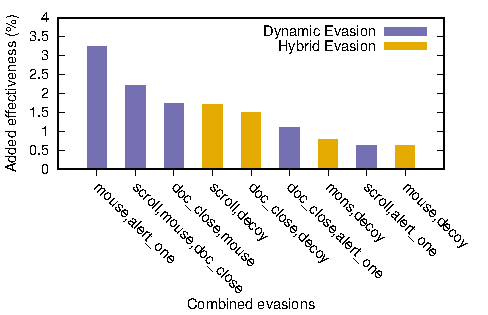
\includegraphics{figures/added-eff}
    \caption{Evasions that have greater than 0.5\% added effectiveness.}
    \label{fig: added eff}
\end{figure}

Interestingly, combining multiple static evasions does not cause any added effectiveness, suggesting that a single static evasion is sufficient to fool scanners susceptible to this kind of evasion.
Furthermore, all combined dynamic evasions in Figure~\ref{fig: added eff} result from combining UI-based evasions, showing that an evasion that requires a more complicated user interaction is more successful.


\subsection{RQ6: Influence of Exploits and Payloads on Evasion Effectiveness}
\label{ss: influence of exploit effectiveness}

The effectiveness of an evasion may depend on the specific exploit or payload used in a malicious document.
For example, consider an exploit that relies on malicious JavaScript and therefore may be detected by scanners that check the JavaScript code in a document.
For such an exploit, a JavaScript-based evasion may work particularly well, because the evasion reduces the chance that scanners identify the document as malicious.
The following studies to what extent the effectiveness of an evasion depends on the exploit or payload used in the malicious document (RQ6).
To this end, we compute the effectiveness of each evasion for the subset of all documents that use a particular exploit or payload.

\subsubsection{Influence of Exploit}

Figure~\ref{figure:toolbutton projection} shows the evasion effectiveness for documents with the ``Toolbutton'' exploit.
The evasions related to JavaScript obfuscation work particularly well, 
since this exploit is based on malicious JavaScript code only, i.e., no other objects, such as fonts or images, are needed.
Many of these evasions are greater than 80\% effective.
The sudden drop in the effectiveness of static and hybrid evasions is also due to the drastically higher success of JavaScript obfuscation-based versus PDF obfuscation-based evasions.

The evasion effectiveness for documents based on the ``Cooltype'' exploit is shown in Figure~\ref{figure:cooltype projection}.
We use the same order of evasions as in Figure~\ref{figure:toolbutton projection} to enable a comparison between the two exploits.
The results show several interesting effects.
First, the most effective evasions for the ``Toolbutton'' exploit reach almost 100\% effectiveness, whereas the peak effectiveness of ``Cooltype''-based documents is only around 75\%.
The reason is that ``Cooltype'' requires both malicious JavaScript code and a malicious font file to be embedded in the PDF.
As a result, none of the static evasions alone is highly effective at hiding ``Cooltype''-based documents.
Second, the effectiveness of evasions based on PDF obfuscation are higher for ``Cooltype'' than for ``Toolbutton'' (the second half of static evasions' bars in the figure).
This result suggests that many scanners identify the exploit by searching for the
malicious font file and thereby make those evasions effective that change the signature of
the PDF document (and hence the signature of the embedded font file).


\subsubsection{Influence of Payload}

With the same approach as exploits, we study the dependence of the evasions on the payload.
We compute the effectiveness of the subset of the samples with each of the three payloads.
In contrast to the exploits, we do not observe any major differences in effectiveness of the evasions.

\medskip
\noindent
Overall, studying the influence of exploits and payloads on the effectiveness of evasions shows that exploits and evasions may influence each other.
Developers of PDF scanners should be aware of this influence when developing anti-evasion techniques, as an attacker might choose suitable evasions depending on how a PDF exploit works.


\section{Discussion}
\label{ss: discussion}

In this section, we discuss how security scanners can defend against evasions (Section~\ref{ss:anti-evasion})
and what limitations our work currently has (Section~\ref{ss:extension}).

\subsection{Mitigating Evasions}
\label{ss:anti-evasion}

One way to mitigate dynamic evasions is to adapt general anti-evasion techniques from other domains to the problem of analyzing PDF documents.
Several recent papers propose to load a potentially malicious file in environments targeted at revealing the malicious behavior of the file.
For example, FuzzDroid~\cite{rasthofer2017making}, IntelliDroid~\cite{wong2016intellidroid}, and SmartDroid~\cite{zheng2012smartdroid} try to cause a potentially malicious Android app to reach ``sensitive'' API calls that would reveal malicious behavior, such as sending an SMS to a premium number.
Adapting this technique to PDF scanners requires identifying sensitive APIs in PDFs.
For known exploits, such APIs may be known, e.g., it is known that the ``Toolbutton'' exploit relies on calling the \code{app.addToolButton} API.
Finding sensitive APIs for previously unknown exploits remains an open research problem.
A related technique to cope with dynamic evasions is to explore multiple execution paths for branch decisions that depend on the environment in which a file is executed.
Rozzle~\cite{rozzle-de-cloaking-internet-malware-2} proposes this idea for client-side JavaScript code.
Adapting their approach is a promising direction for mitigating the environment-related dynamic evasions.

To deal with UI-related evasions, dynamic scanners could adapt ideas used in PuppetDroid~\cite{gianazza2014puppetdroid} and PyTrigger~\cite{fleck2013pytrigger}.
These approaches record an interaction trace from a human and play it back when loading the file under analysis to get through possible checks that guard the attack.
One of the dynamic scanners studied in this work, Cuckoo, mitigates evasions using a simpler form of this idea: The scanner arbitrarily moves the mouse to simulate a human user~\cite{cuckoo_mouse_movement}.
However, this mitigation technique is unlikely to work for evasions that require a more complicated user interaction, such as a ``captcha''.

To identify files that behave differently in an analysis environment, some techniques compare the execution behavior of the file in several different environments, e.g. virtual and physical~\cite{balzarotti2010efficient}.
Another kind of anti-evasion technique is to hide any difference between a virtual and a physical execution environment to fool the evasive malware~\cite{shi2018handling}.
%
Finally, to deal with the large number of possible evasions and combinations of evasions, training machine learning models to distinguish benign from malicious files seems to be a worthwhile direction~\cite{smutz2012malicious,vsrndic2013detection,laskov2011static,corona2014lux0r}.
The main challenge for effectively training machine learning models is to obtain a sufficiently large set of labeled data.
Our framework could serve as a generator of malicious training files that use different evasions and combinations of evasions.

The high recall of SAFE-PDF~\cite{2018arXiv181012490J}, which is based on abstract interpretation of JavaScript code embedded in PDFs, shows that conservative program analysis may provide an effective way of detecting malicious behavior despite evasions. The downside of any conservative program analysis are spurious warnings, which the relatively high false positive ratio of SAFE-PDF confirms.



\subsection{Choice of Scanners}
\label{ss:extension}

We focus on in-production, commercial security scanners because they represent the current state-of-the-practice, and recent academic scanners because they represent the state-of-the-art.
The studied scanners contain more static than dynamic scanners because static scanners currently dominate the market.
For example, the VirusTotal service aggregates more than 60 static scanners at the time of writing this paper~\cite{vt_engines_count}, whereas we could find only ten commercial dynamic scanners, out of which three consented to participate in this research.

Our work should not be understood as a comparison of different scanners, but rather as a comparison of each scanner's effectiveness before and after adding evasions.
The version of the scanners used in online aggregation services, which we use for the studied static scanners, may differ from the full-fledged scanners, because vendors may optimize the response time for an online service~\cite{pitfall}.



\section{Conclusion}
\label{sec_conclusions}

Our work consists of two studies that quantitatively and qualitatively investigate the influence of a CI service (e.g., \textsc{TravisCI}), and CI as a practice, on the time-to-delivery of merged PRs, respectively. In our quantitative study, we analyze 162,653 PRs of 87 GitHub projects to understand the factors that influence (and improve) the delivery time of merged PRs. In our qualitative study, we analyze 450 survey responses from participants of 73 projects (out of the initial 87 projects). We investigate the perceived influence of CI on the delivery time of merged PRs. We also study the perceived influence of CI on the code review and release processes.

As a key takeaway, our studies demonstrate that the adoption of \textsc{TravisCI}
will not necessarily deliver or merge PRs more quickly. Instead, the pivotal benefit of a CI service is to improve the mechanisms by which contributions to projects are processed (e.g., facilitating decisions on PR submissions), without compromising the quality of the project or overloading developers. The automation provided by CI and the boost in developers' confidence are key aspects of using CI. For instance, CI may help the process of sorting which PRs are worth reviewing (e.g., PRs with green builds).
Furthermore, open-source projects wishing to attract and retain external contributors should consider the use of CI in their pipeline, since CI is perceived to lower the contribution barrier while making contributors feel more confident and engaged in the project.

\section*{Acknowledgments}
\label{sec_Acknowledgments}

This work is partially supported by INES (\url{www.ines.org.br}), CNPq grants 465614/2014-0 and 425211/2018-5, CAPES grant 88887.136410/2017-00, FACEPE grants APQ-0399-1.03/17, and PRONEX APQ/0388-1.03/14.

\section*{Data Availability}
For replication purposes, we publicize our datasets and results to the interested researcher: \url{https://prdeliverydelay.github.io/#datasets}

\section*{Declarations}

\textbf{Conflict of interests}. The authors declare that they have no conflict of interest.


%% The next two lines define the bibliography style to be used, and
%% the bibliography file.
\bibliographystyle{ACM-Reference-Format}
\bibliography{main}

\appendix
\section{Dynamic Smagorinsky Model}
\label{app:dynsmago}

Germano et al. proposed in \cite{germano1991dynamic} an improvement to the standard Smagorinsky model by setting the Smagorinsky constant $C_s$ not to a fixed value set a priori, but rather to adapt it dynamically in space and time dependent on the current state of the flow.
This dynamic procedure is based on applying a test filter $\widehat{(\cdot)}$ to the solution.
The LES solution can then be used to compute the resolved stress tensor
\begin{equation}
  L_{ij} = \widehat{\widetilde{u}_i \widetilde{u}_j} - \widehat{\widetilde{u}}_i \widehat{\widetilde{u}}_j,
\end{equation}
which entails the subgrid stresses induced by the test filter.
Germano's identity finds a correlation between those resolved subgrid stresses and the unknown subgrid stress induced by the LES filter.
Lilly \cite{lilly1992proposed} proposed a least-squares approach to compute $C_s^2$ such that Germano's identity is optimally obeyed, which gives
\begin{equation}
  C_s^2 = \frac{\langle L_{ij}M_{ij}\rangle_{avg}}{\langle M_{ij}M_{ij} \rangle_{avg}}.
  \label{eq:dynsmago_ls}
\end{equation}
Here, $\langle\cdot\rangle_{avg}$ denotes some averaging operation to avoid extremely large coefficients and thus to stabilize the model.
The tensor $M_{ij}$ is shorthand for the expression
\begin{equation}
  M_{ij} = 2 \Delta^2 \widehat{\sqrt{2\tilde{S}_{kl}\tilde{S}_{kl}}\,\tilde{S}_{ij}}  - 2 \widehat{\Delta}^2 \sqrt{2\widehat{\tilde{S}}_{kl}\widehat{\tilde{S}}_{kl}}\, \widehat{\tilde{S}}_{ij},
\end{equation}
with $\widehat{\Delta}$ as the filter width of the test filter and with the rate-of-strain tensor on the test filter level $\widehat{\tilde{S}}$ computed analogously to \eqref{eq:smago} based on the test-filtered velocity field $\widehat{\tilde{u_i}}$.

In the DG context, the dynamic procedure is applied in an elementwise fashion.
As test filter $\widehat{(\cdot)}$ with filter width $\widehat{\Delta}$, we apply a modal cut-off filter to the solution polynomial with a degree of $N_{test}=2$ and $N_{test}=3$ for the cases employing a polynomial degree of $N=5$ and $N=7$, respectively.
Moreover, the averaging operator $\langle\cdot\rangle_{avg}$ for the numerator and denominator in \eqref{eq:dynsmago_ls} is chosen as an average in each element yielding a single coefficient $C_s^2$ for each element.
The resulting eddy-viscosity is then clipped to the range $\mu_t \in [-100\mu,1000\mu]$ with respect to the physical viscosity, since the unclipped model produced from time to time a few huge values for $C_s^2$, which deteriorated the solution quite drastically.
The clipping range itself seemed to have only very limited influence on the model's behavior in our tests and provided very similar results for a wide range of different clipping intervals.



\end{document}
\endinput
\section{Identifying Macro Norm violating comments}
Our aim is to identify macro norm violating comments on Reddit, to quantify their prevalence, and to characterize their content, rate of engagement, and language usage. However, there are too many comments for manual annotation, and state-of-the-art machine learning classifiers are not robust enough on their own. We overcome these issues using a human-AI pipeline in which we use classifiers with a high recall to nominate candidate comments that might be violating, and then focusing our manual annotations with trained annotators on these nominated comments. By tuning the classifiers to have high recall over high precision, our pipeline ensures that almost all of the violating comments are sent to be reviewed by our annotators. Additionally, in concurrence with prior work \cite{chandrasekharan2019crossmod, seering2020reconsidering}, this pipeline ensures that a human has the final say in labeling any piece of content as a violation.

In this section, we first discuss the scope of our investigation, including how we define violating comments for this paper. We then summarize our pipeline for identifying violating comments. 

\subsection{Scope of the Study}

% \usepackage{booktabs}
% \usepackage{vcell}


\begin{table}[tb]
\centering
\caption{The eight macro norm violations on 97 popular subreddits and their definitions. We took the norms uncovered in a prior study \cite{Chandrasekharan2018internet} and expanded on some of their definitions to better fit our data.}
\begin{tabular}{ll}
\multicolumn{1}{c}{\textbf{MACRO NORM VIOLATIONS}}                                                & \multicolumn{1}{c}{\textbf{EXAMPLE COMMENTS}}                                                                                                                                         \\ 
\toprule
\vcell{Using misogynistic or vulgar slurs}                                                        & \vcell{\textit{"god... I want sage to knock this c*** out"}}                                                                                                                          \\[-\rowheight]
\printcelltop                                                                                     & \printcelltop                                                                                                                                                                         \\
\vcell{Inflammatory political claims}                                                             & \vcell{\begin{tabular}[b]{@{}l@{}}\textit{"a day old troll complaining about liberals -- I }\\\textit{smell a lost trumpkin"}\end{tabular}}                                           \\[-\rowheight]
\printcelltop                                                                                     & \printcelltop                                                                                                                                                                         \\
\vcell{Bigotry}                                                                                   & \vcell{\begin{tabular}[b]{@{}l@{}}\textit{"punishment for not being hateful enough and }\\\textit{not destroying the gays"}\end{tabular}}                                             \\[-\rowheight]
\printcelltop                                                                                     & \printcelltop                                                                                                                                                                         \\
\vcell{\begin{tabular}[b]{@{}l@{}}Verbal attacks on Reddit or specific \\subreddits\end{tabular}} & \vcell{\begin{tabular}[b]{@{}l@{}}\textit{"also reddit sucks because a user making~an~error }\\\textit{refuses to delete their post and redo it }\\\textit{correctly"}\end{tabular}}  \\[-\rowheight]
\printcelltop                                                                                     & \printcelltop                                                                                                                                                                         \\
\vcell{Posting pornographic links}                                                                & \vcell{\textit{[URL]}}                                                                                                                                                                \\[-\rowheight]
\printcelltop                                                                                     & \printcelltop                                                                                                                                                                         \\
\vcell{Personal attacks}                                                                          & \vcell{\textit{"you know man youre kind of a f***ing d*****"}}                                                                                                                        \\[-\rowheight]
\printcelltop                                                                                     & \printcelltop                                                                                                                                                                         \\
\vcell{Abusing and criticizing moderators}                                                        & \vcell{\textit{"the mods in this sub need to wake the f*** up"}}                                                                                                                      \\[-\rowheight]
\printcelltop                                                                                     & \printcelltop                                                                                                                                                                         \\
\vcell{\begin{tabular}[b]{@{}l@{}}Claiming the other person is too \\sensitive\end{tabular}}      & \vcell{\textit{"get off the internet with your sensitive ass"}}                                                                                                                       \\[-\rowheight]
\printcelltop                                                                                     & \printcelltop                                                                                                                                                                         \\
\bottomrule
\end{tabular}
\end{table}

Reddit, the focus of our study, is a large-scale social media platform with 52 million daily active users \cite{59_Phan}. On Reddit, users join smaller subcommunities called subreddits that cover a specific topic and are managed by voluntary moderators who enforce community-specific rules (e.g., the type of allowed content, expected member behaviors), making the platform a good test-bed for studying user behaviors across diverse sets of moderation strategies and topics. In particular, we explore comments posted in response to top-level post submissions as most of the discussions on Reddit take place in the comment section. Given that the subreddits each have varying rules, we consider a comment to be violating if it breaks one of the \textit{macro norms} on Reddit --- norms that the vast majority of subreddits agree on. These norms were identified in prior work~\cite{Chandrasekharan2018internet} that investigated the 100 most popular subreddits harboring nearly a third of all comments on Reddit to extract the topic categories for the moderated (summarized in Table 1). 

We rely on macro norms as they provide us with a lens to measure the prevalence of violating comments that are largely independent of community-relevant contexts. However, in doing so, we are explicitly not accounting for comments that do not violate macro norms but still violate local rules of the respective subreddit. We also note that some subreddits have explicitly chosen to permit content that violates one or more of these macro norms (e.g., vulgar or sexualized comments). This highlights an important tension between the local and the macro norms. We discuss these issues and expand on their implications for future content moderation in the discussion section.


\subsection{Data for Training and Testing the Classifiers}
The first step of our pipeline uses a set of machine learning classifiers to flag comments that are potentially macro norm violations. We trained and tested these classifiers following best practice by constructing a balanced dataset that contains an equal number of moderated comments (denoted as $\mathcal{M}$) and unmoderated comments that are still online and were not moderated or deleted by the author (denoted as $\mathcal{M'}$). There are more unmoderated than moderated comments on Reddit---$\mathcal{M'}$, therefore, is a subset of all unmoderated comments. While such balanced datasets do not match the real-world distribution, balancing the dataset gives the resulting model equal priority to each class, which is important for ensuring that our model actually learns the meaningful features for the classification task and not just the uneven class distribution. 

\subsubsection{\rnr{$\mathcal{M}$: moderated comments}} 
$\mathcal{M}$ represents the top 100 most popular English subreddits during the 11 month period from May 2016 to March 2017. Given that the moderated comments are removed soon after they are posted, prior work used \textit{praw}, a Reddit streaming API, to stream and save all comments posted to each of these study subreddits before they were moderated \cite{Chandrasekharan2018internet}. 24 hours after each of these comments were streamed, all comments were queried again via the API using their unique \textit{comment\_ID} and verified which of them were replaced by a [``removed''] tag as that would signal their removal due to moderation. Any comments by AutoModerator accounts, which are bots for moderation, were removed from $\mathcal{M}$. This left $\mathcal{M}$ with a total of 2,831,664 removed comments, with at least 5,000 for each of the 100 study subreddits. 


\subsubsection{\rnr{$\mathcal{M'}$: unmoderated comments}} 
As $\mathcal{M}$ contained only the moderated comments from the sampling period, we collected $\mathcal{M'}$ ourselves through historical archives of Reddit comments. Of the 100 study subreddits from $\mathcal{M}$, three--- r/The\_Donald, r/Incels, r/soccerstreams---no longer exist on the platform, so we focused our investigation on the remaining 97 study subreddits. During the construction of $\mathcal{M'}$, we aimed to closely replicate the data collection process of $\mathcal{M}$. For each of the 97 subreddits, we used \textit{Pushshift} dataset that stores all content posted on the Reddit platform to gather IDs of submissions that were posted from the same timeframe as when $\mathcal{M}$ was collected with an even distribution across the 11 months. We then used \textit{praw} to get the actual comments with the submission IDs and discarded any that were posted by a bot or moderated. We continued this process until we had a balanced dataset for each of the 97 study subreddits.




\begin{figure}[tb]
  \centering
  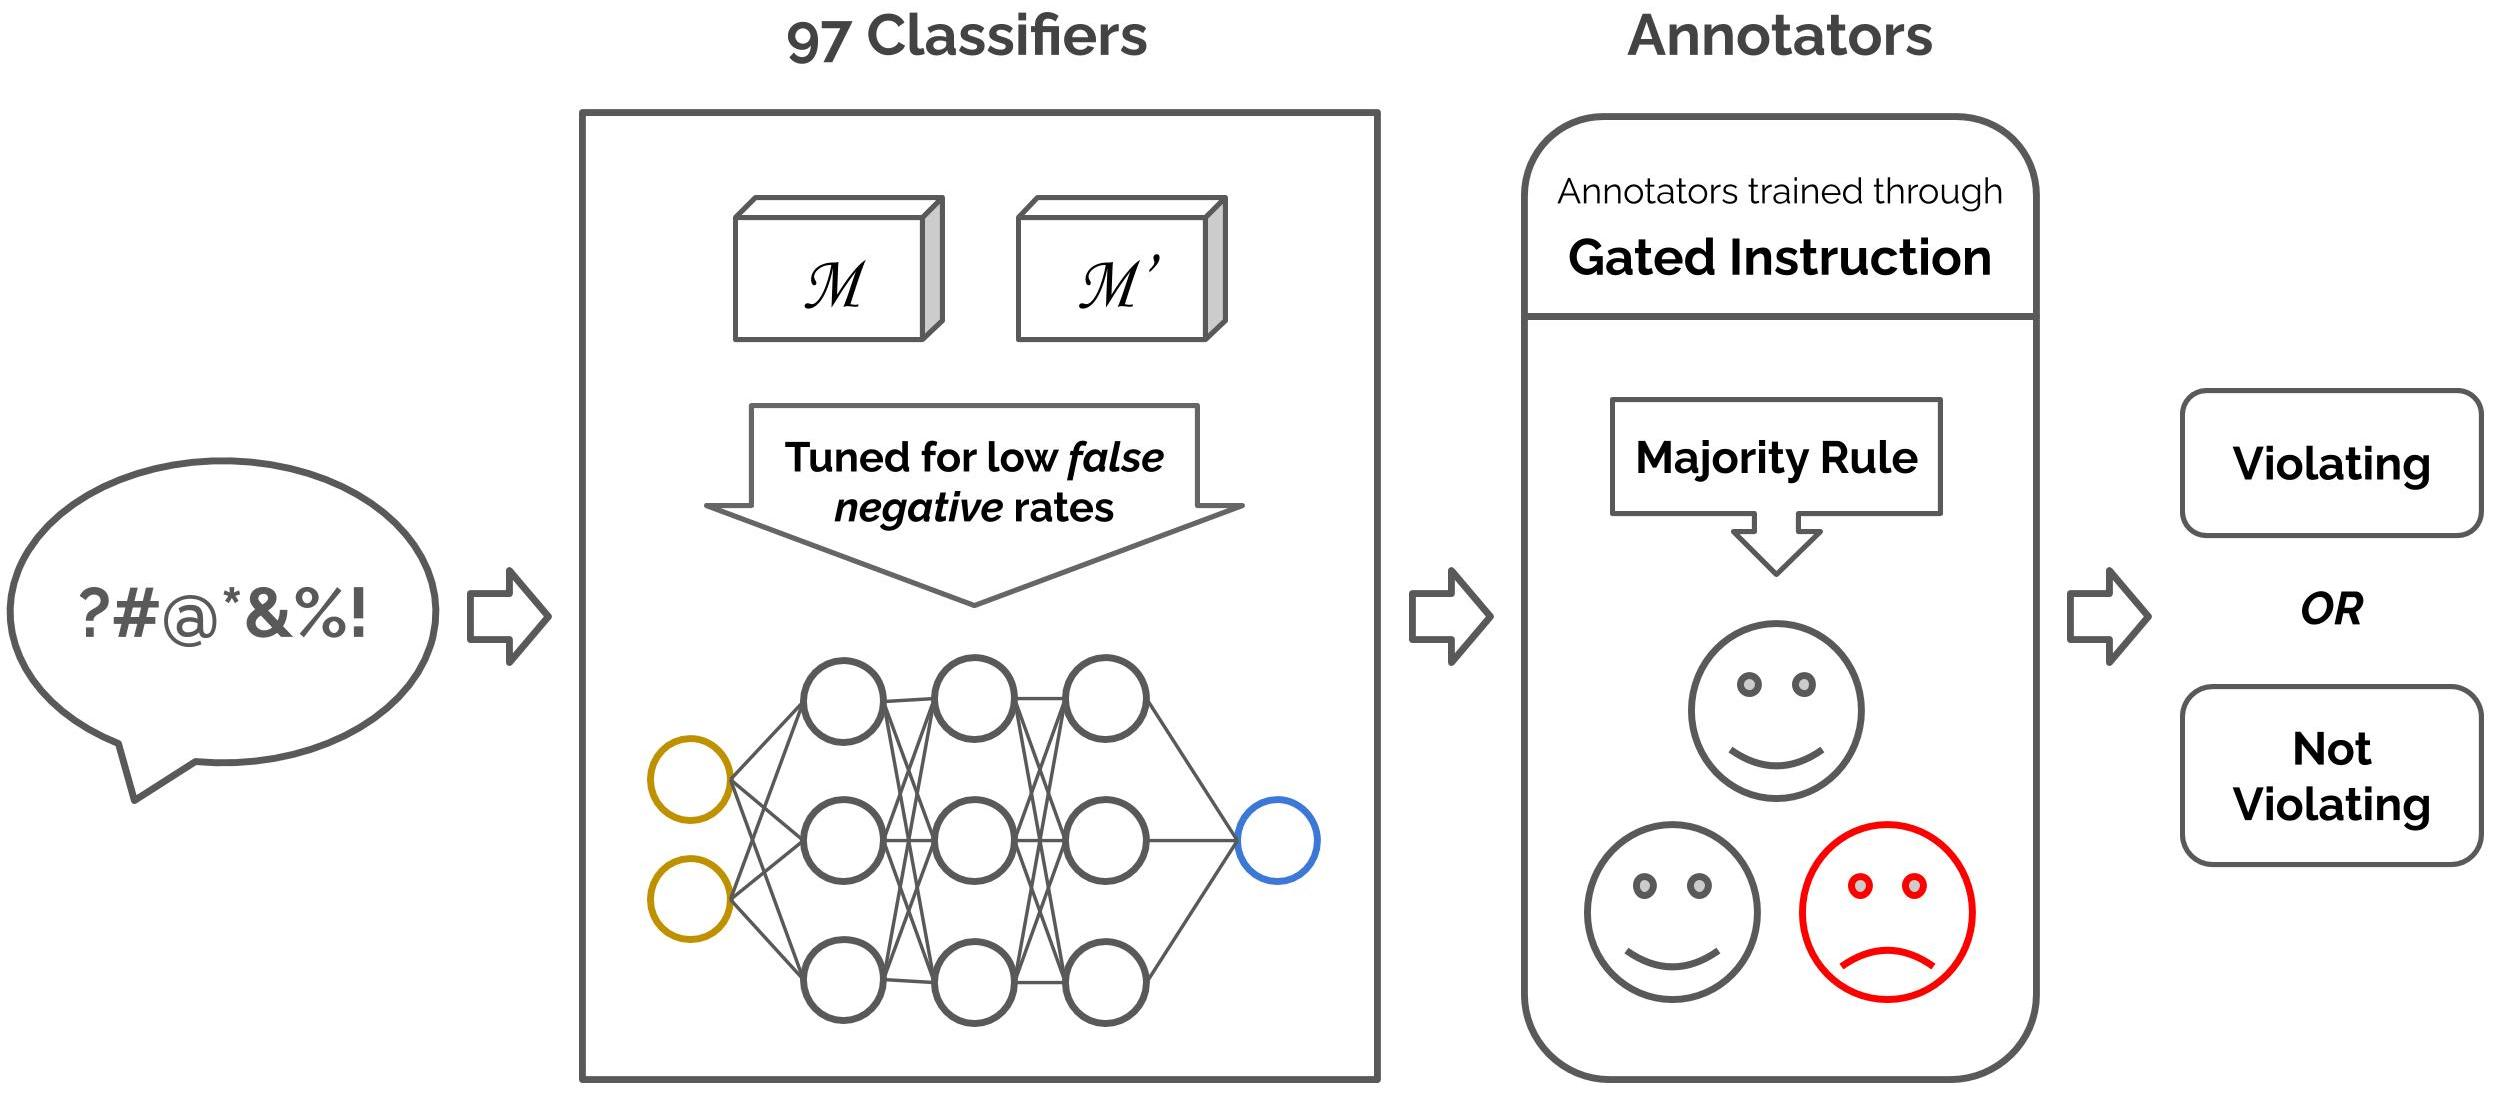
\includegraphics[width=0.90\textwidth]{content_minor_revision__Apr2022/images/Final_pipeline.jpg}
  \caption{An illustration of the human-AI pipeline for identifying violating comments. Our pipeline includes 97 subreddit classifiers that are trained using a balanced dataset of moderated and unmoderated comments, and human annotators who are trained through gated instruction~\cite{25_Liu}. Our classifiers (tuned for high recall) nominate potentially violating comments and human annotators make the final determination.}
  \Description{Human-AI pipeline}
\end{figure}




\subsection{Building the Classifiers}
Using $\mathcal{M}$ and $\mathcal{M'}$, we built 97 neural network binary classifiers, each of which was trained on the data from one of the 97 study subreddits to classify whether a given comment would be moderated on that subreddit. These classifiers collectively determine whether a comment is likely to have violated one of the macro norms and thus would have been removed on most of the subreddits. We refer to these classifiers as subreddit classifiers. 

\subsubsection{Preprocessing the data} 
We first preprocessed our dataset by putting all characters in lowercase and removing non-alphabetical characters. We then segmented our dataset into a \textit{training} dataset (70\% of all data) and \textit{testing} and \textit{validation} datasets (15\% of all data each), each with an equal number of moderated and unmoderated comments. For every study subreddits, we then used our training dataset to train word embeddings from scratch and encoded comments as fixed-length vectors, trancating and padding as needed. 

\subsubsection{Building the classifiers} 
We built our classifiers using Google's \textit{TensorFlow} and trained and validated them with the encoded dataset. The classifiers have a four-layer neural network architecture, starting with an embedding layer that takes the encoded list of integers and finds an embedding vector for each word, which we learned as we trained our network. We then pass through an average pooling layer that returns a fixed-length output vector and then through a dense layer with Rectified Linear Unit (ReLU) activation function \cite{26_TensorFlow}. Finally, we employ another dense layer with a sigmoid activation function that transforms the final output of the network into a value between 0.0 and 1.0. For our binary classification task, we identify a comment as one that would have been removed in a given subreddit if the final output of the network is greater than or equal to 0.5. 

We then fine-tuned the following four parameters for each of our subreddit classifiers using grid search where we try out exhaustive combinations of hyperparameters given candidate values:  the size of the word index used in the encoding, the length of the input vector, the number of epochs during the training phase, and the number of nodes for the ReLU layer of the neural network. These are summarized in Table 2. We optimized for the F1 score (\textit{f}-measure) on our validation dataset, achieving an average of 72.3 (std=4.32) across the 97 classifiers. This is comparable to the classifiers presented in prior work that were trained on a similar dataset \cite{4_Chancellor, chandrasekharan2019crossmod}.


% \usepackage{booktabs}


% \usepackage{booktabs}


\begin{table}[tb]
\centering
\caption{Parameters and the values used for them to fine-tune the classifiers}
\begin{tabular}{ll}
\multicolumn{1}{c}{\textbf{DESCRIPTION} } & \multicolumn{1}{c}{\textbf{SET OF VALUES} }  \\ 
\toprule
Size of the word index                    & {[}10000, 44000]                             \\
Max length of the input                   & {[}256, 512]                                 \\
Number of epochs during the training      & {[}30, 40, 50]                               \\
\# of nodes for the ReLU layer            & {[}16, 32]                                   \\
\bottomrule
\end{tabular}
\end{table}

% \begin{table}
% \centering
% \caption{Parameters and the values used for them to fine-tune the classifiers}
% \begin{tabular}{lll}
% \multicolumn{1}{c}{\textbf{PARAMETERS}} & \multicolumn{1}{c}{\textbf{DESCRIPTION}} & \multicolumn{1}{c}{\textbf{SET OF VALUES}}  \\ 
% \toprule
% \textit{$\mathcal{WI}$}                             & Size of the word index                   & {[}10000, 44000]                            \\
% \textit{$\mathcal{ML}$}                             & Max length of the input                  & {[}256, 512]                                \\
% Epochs                                  & Number of epochs during the training     & {[}30, 40, 50]                              \\
% \textit{$\mathcal{DN}$}                             & \# of nodes for the ReLU layer           & {[}16, 32]                                  \\
% \bottomrule
% \end{tabular}
% \end{table}


\subsection{Machine Learning Flags Comments}
We marked a comment as \textit{flagged} (potentially norm violating) if the number of subreddit classifiers that flagged the comment, which we call the \textit{classifier agreement score}, was greater than or equal to 80 out of 97. This threshold was selected to achieve a high recall on the ensemble classifier even at the cost of producing false positives as our pipeline includes human annotators who validate the classifier flagged comments. In other words, we wanted our process to miss as few violating comments as possible, so we deliberately used a low threshold of 80 out of 97 and passed these comments to a human review stage. This approach provides statistical power even within a realistic budget for manually annotating comments, because it results in roughly one in five flagged comments later being coded as a violation while maintaining a near-zero false negative rate.

We confirmed that this threshold indeed captures most of the violating comments: the first author manually annotated a random sample of 1,000 comments in the validation dataset from 2016 to 2017 period. This sample contained 400 comments with $< 80$ subreddit classifier agreement, 200 with $80 \leq \text{agreement} < 85 $, 200 with $85 \leq \text{agreement} < 90$, and 200 with $\geq 90$ agreement. We find that only one percent of the comments with $< 80$ classifier agreement violated at least one of the macro norms when manually inspected, whereas this number significantly increased in the subsequent sample groups (9.5\%, 12\%, and 28\% in the order of increasing classifier agreement). This low false negative rate when using a low enough agreement threshold matches the observations in a prior work that took a similar approach to classifying violating comments on Reddit \cite{chandrasekharan2019crossmod}.

In addition, to confirm that our classifier's low false negative rate holds for the comments from 2020 period, we further annotate 400 comments with classifier agreement score of less than 80 from this period randomly sampled across the study subreddits. We find our result to replicate, with roughly the same rate of 1.25\% of the sample to violate one of the macro norms. Although our subreddit classifiers were trained on comments from a 2016 to 2017 period, this low false negative rate for the comments from 2020 suggests that when combined with our human annotators, our overall pipeline still remains robust even for the newer comments. Finally, as we describe in the following section on our bootstrap sampling methods, these false negative rates are accounted for in our calculation of the confidence interval of our estimations.


\subsection{Human Annotation Validates the Flagged Comments}
\label{sec:annotation}
The tradeoff for tuning our classifiers for very few false negatives is that they produce more false positives. So we recruited human annotators to verify that the classifier flagged comments are indeed violating by asking them to code a subset of the flagged comments to see which macro norms they violate, where the subset was a random sample of the flagged comments with an even distribution across the 97 study subreddits. The definitions of these macro norms that we presented to our annotators were inspired by prior work~\cite{Chandrasekharan2018internet}, but based on our qualitative annotation discussed above, we found it appropriate to expand the definitions for some of them to better fit our data. We updated the norm described as ``opposing political views around Donald Trump'' to ``inflammatory political claims'' that covers inflammatory comments that are against the right-leaning and the left-leaning political ideologies and updated the norm described as ``hate speech that is racist or homophobic'' to ``bigotry'' that covers hate speech directed at ethnic or religious groups as well. 


\begin{figure}[tb]
  \centering
  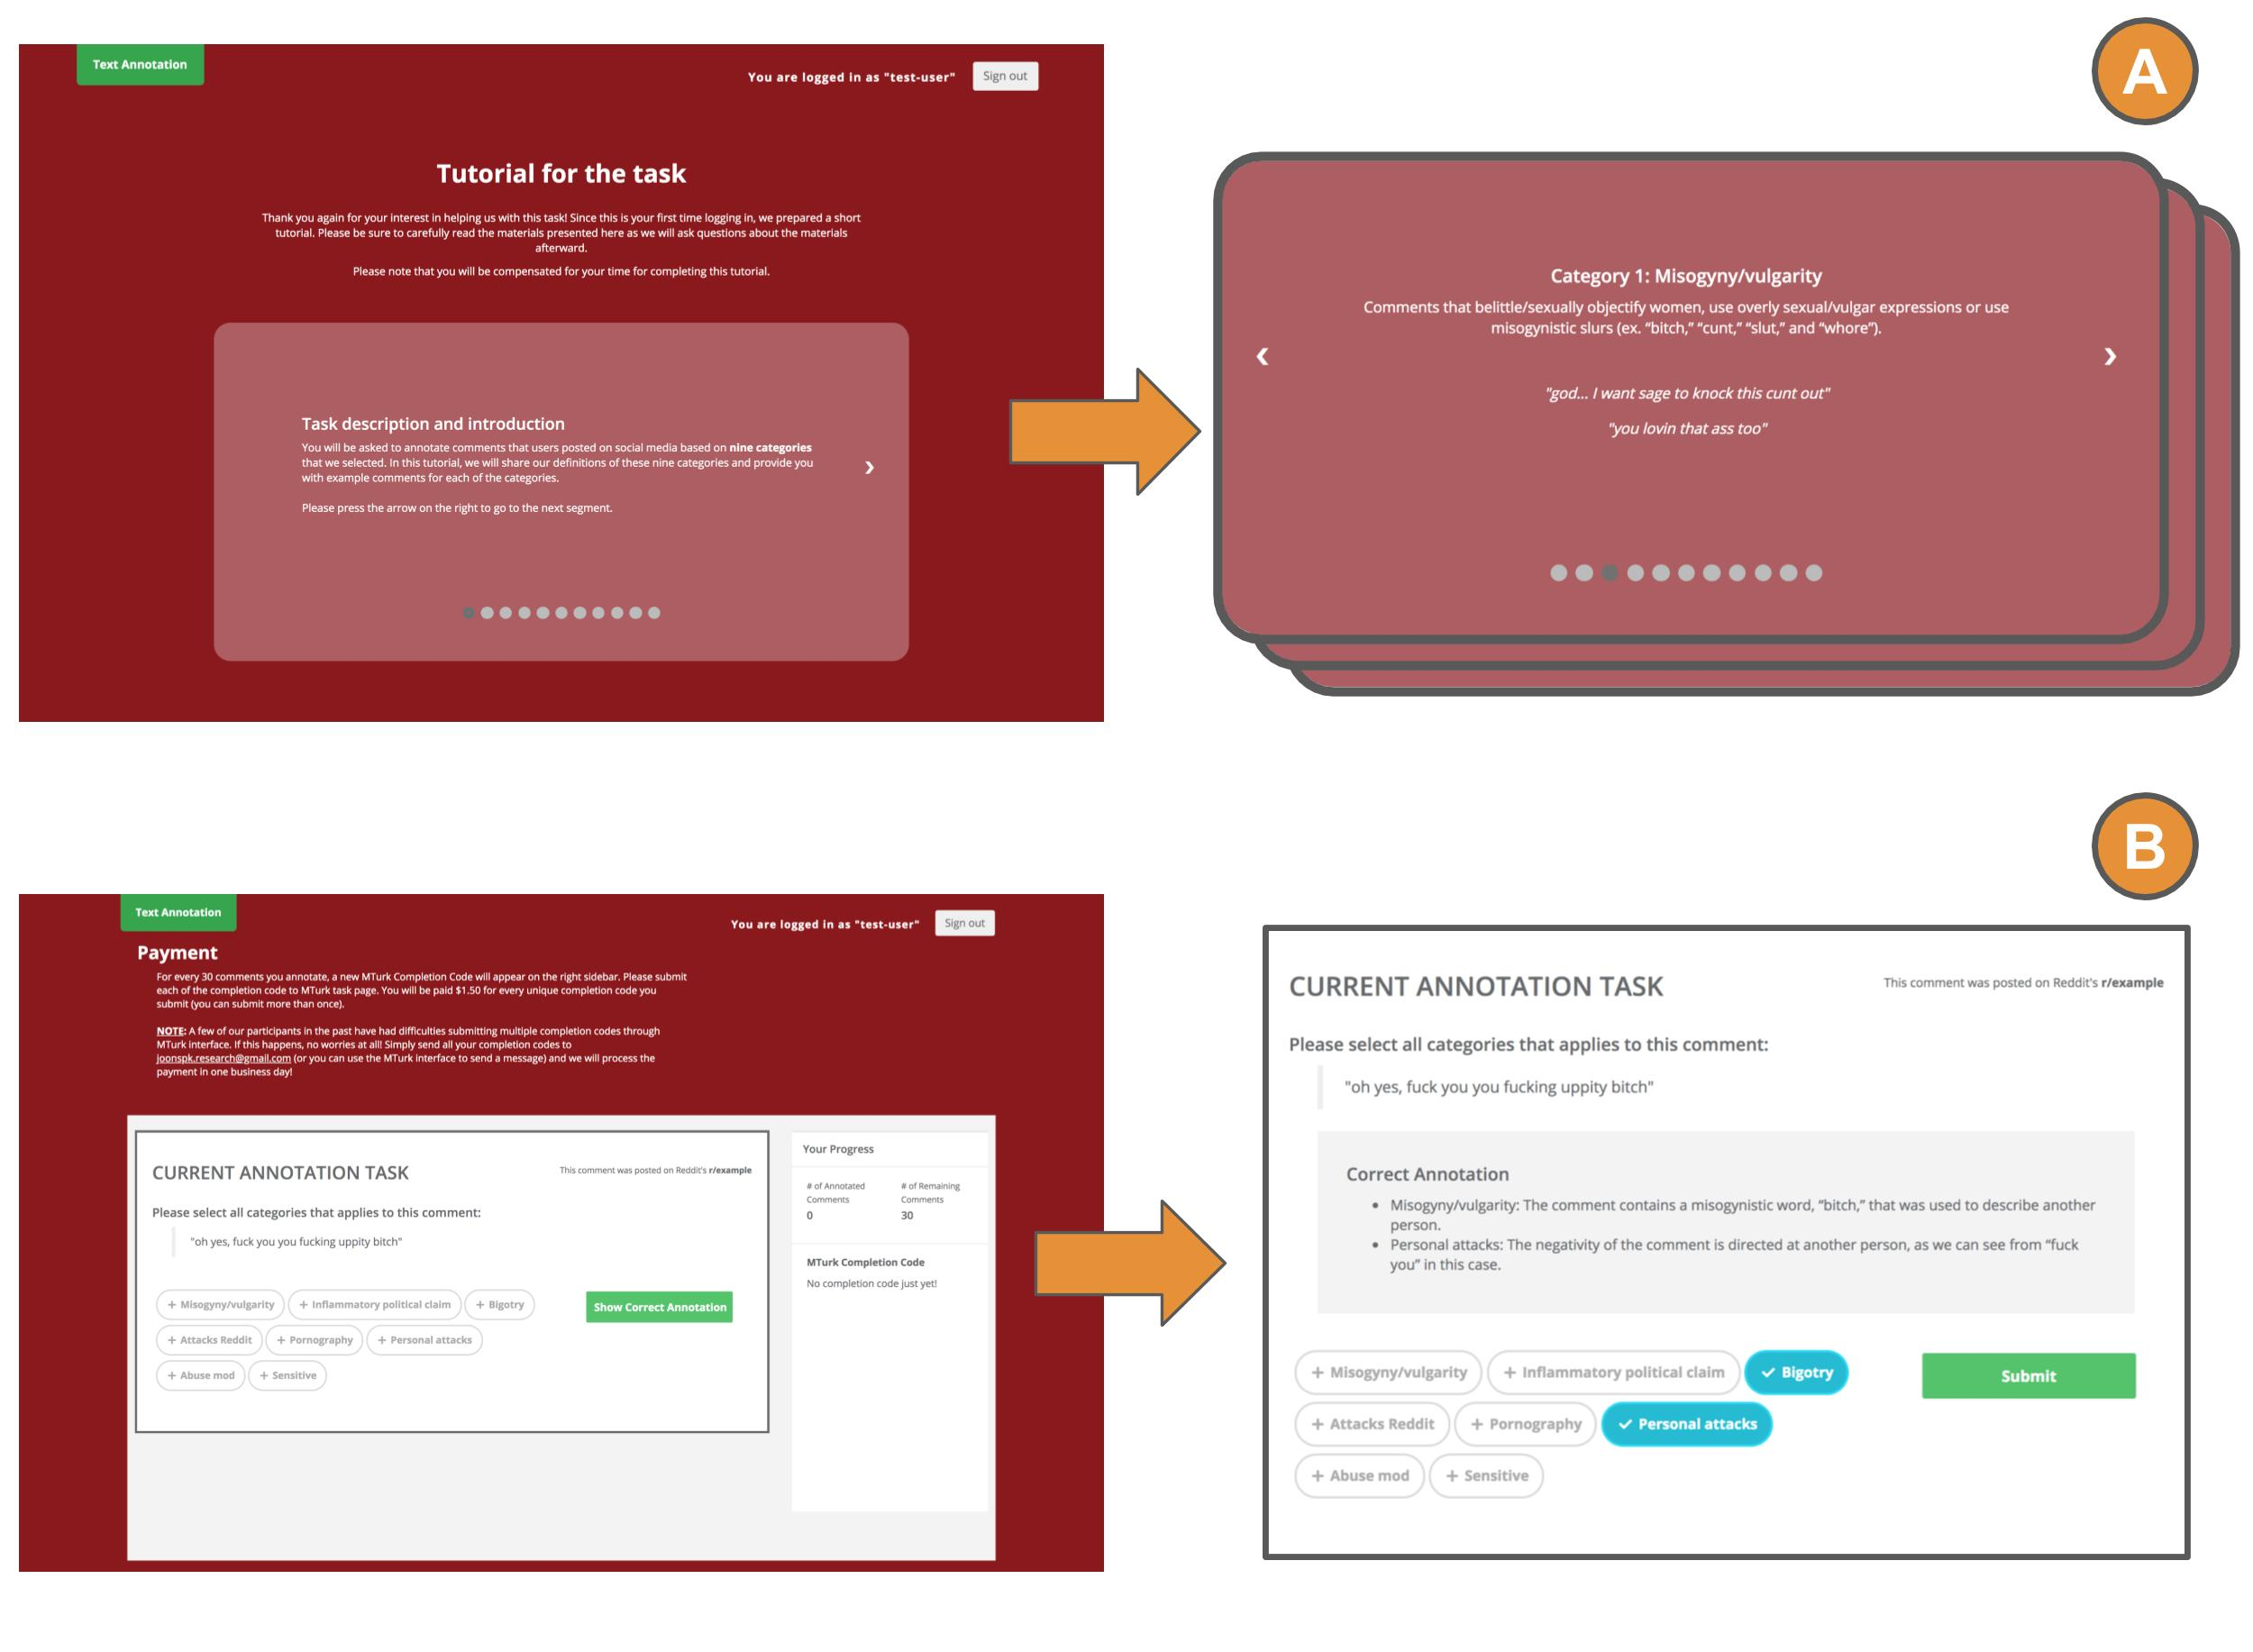
\includegraphics[width=0.98\textwidth]{content_minor_revision__Apr2022/images/annotation_interface.jpg}
  \caption{\textbf{A:} The interface for introducing the task description and eight macro norms to a new annotator. The definitions for each norms are shown one by one, accompanied by gold-standard examples that violate the norm. \textbf{B:} The interface for training and testing new annotators. Once the new annotators select their annotation, the correct annotation is shown accompanied by gold-standard examples. The interface for the main annotation task is the same but without presenting the correct annotation portion.}
  \Description{Annotation Interface}
\end{figure}



\subsubsection{Recruiting  crowd workers} 
The crowd workers were recruited from Amazon Mechanical Turk (MTurk), and they had to be at least 18 years old, living in the US, and have completed more than 1,000 Human Intelligence Tasks (HITs – MTurk’s task unit) with the minimum HIT approval rating of 98\%. In our pilot annotation task that we will describe in a subsequent subsection, our annotators took around 10 seconds (median=9.66 seconds; 75th percentile=16.99 seconds) to annotate a single comment. Based on this, we decided to pay our workers \$1.50 for every 30 comments they annotated to ensure that we are paying the majority of our workers at the rate of at least \$15.00 per hour. We decided on this rate informed by Rolf's \textit{The Fight For Fifteen} \cite{20_Rolf}.

\subsubsection{Human annotation workflow} 
Applying human annotation for non-trivial classification tasks could suffer from inaccurate annotations due accidental errors~\cite{22_Angeli, 23_Pershina, 24_Zhang}. Therefore, we designed a training and a testing phase that are inspired by the \textit{gated instruction} workflow~\cite{25_Liu} as follows to ensure that our annotators clearly understand and are proficient at the task:

Our annotators were directed to a custom-built web platform to which they could sign in with their MTurk ID. For those joining for the first time, they were redirected to the first portion of the training phase in which they were presented with 1) an overview description of the task and its goal, 2) a content warning notifying them that some comments in the task might include offensive language, and 3) the eight macro norms accompanied by their definitions and two gold-standard example comments that we manually chose from the test dataset (Figure 2-A). When they finished reviewing this content, they were asked to practice annotating 30 hand-selected, gold-standard examples of the macro norm violations handpicked from our test dataset. This was done on the actual interface used for the main annotation task that showed a comment to be annotated, and multi-select HTML form for submitting macro norm violations (Figure 2-B). The annotators could select any number of macro norms they thought the given comment violated. Importantly, during this training phase, the workers were presented with the correct annotation and explanation after each time they submitted their annotations for a given comment. Note also that, in order to avoid biasing their decisions by imposing an ``expert'' AI opinion, the workers were not told that the comments were flagged by an algorithm as potentially norm violating \cite{seering2020reconsidering}.

Of the 30 practice comments, the last 10 were effectively the test annotations; we measured our annotators’ Cronbach's alpha reliability score when compared to our gold-standard annotations, and only admitted those whose reliability score was greater than or equal to 0.7 for the last 10 training annotations. All annotators who participated in the training and testing phase were provided with a completion code they could submit to MTurk and were paid \$1.50 for their time. Those who were admitted were allowed to start the main annotation task. They could annotate as many comments as they wanted as long as there were more comments to be annotated, and were provided with a completion code they could submit to receive \$1.50 for every 30 comments they annotated. Each of the comments was seen by three unique annotators to test for majority agreement. 

During the course of this study, we recruited a total of 31 annotators who collectively annotated a total of 4,850 comments. \mrev{Finally, we followed best practices for accounting for annotator well-being during their task. In addition to presenting the aforementioned content warning, we made sure that our annotators could freely leave the study at any time if they felt uncomfortable with the annotation task. We purposefully designed our compensation scheme to ensure that we paid our participants in small increments instead of asking them for a long period of participation before receiving their compensation to ensure that our participants could receive the payment they deserve regardless of when they choose to leave the study.}


\subsubsection{Pilot} 
To confirm the robustness of this approach and  to determine the right level of compensation for the workers, we ran a pilot annotation task for which we recruited 20 annotators to partake in the training phase. Of the twenty, 8 annotators passed the testing phase and went on to annotate 194 randomly selected comments from the test dataset. The first author manually annotated the 194 comments that the annotators annotated during the aforementioned pilot tasks to establish baseline annotations to which annotators' work would be compared. In relation to the first author’s manual annotation, the majority-agreed annotation of the annotators yielded a Cronbach's alpha score of 0.86. 

\section{Discussion}
The contribution we make in this paper is twofold. First, we present a large-scale analysis that investigates the prevalence and characteristics of macro norm violating comments that are left unmoderated on Reddit. In doing so, we provide the social computing literature with empirical results that can help aid policies, moderation, and design interventions. These results illustrate how roughly one in every 20 comments on Reddit violates the platform's own expectations of what should not be present, and shines light on the the most prevalent types of violations. Second, we demonstrate a materialized human-AI-bootstrap pipeline for identifying violating comments. We use classifiers trained on a dataset of previously moderated comments on the 97 most popular subreddit communities on Reddit to triage potentially violating comments at scale, employ trained human annotators to validate a sample of the classifiers’ decisions, and calculate the final estimation and our confidence using the bootstrap resampling technique.

In the remainder of this section, we discuss what our findings may mean for social media and for efforts to rein in anti-social behavior online; we try to interpret what the rate of violating comments in the 4\% to 6\% range means in reality, and scope out what can be inferred from our results. Finally, we end with our work’s limitations and potential avenues for future research. 


\subsection{Is This Result Good, Bad, or Neither?}
Comments that violated the macro norms were prevalent on the study subreddits during both time periods. As noted in the introduction, even Facebook's transparency report of 0.1\% of its content being categorized as hate speech~\cite{58_Culliford, 91_Barrett} raised concerns as it translates to affecting millions of users. Given this, 4\% to 6\% of norm violating comments likely is not a small amount. Also, the overall rate of moderation, though has increased over the years perhaps in some part due to the growing awareness of the negative impacts these content can have, remains low with one in twenty of the norm violating comments in 2016, and one in ten in 2020, being removed by the moderators. These rates are comparable to the 3--5\% rate of hate speech moderation reported in Facebook’s internal documents that were made public in recent whistleblower exposures \cite{facebook_scandal, facebook_scandal_2}. This provides an important context for both our findings and those in Facebook’s internal documents; that these two findings covering very different contexts and likely, using diverging methods of measurement (it is unclear how Facebook measured their moderation rate), are roughly converging may illustrate a broader point about the challenges of today’s large-scale content moderation.

\mrev{It is also worth highlighting that for many communities we studied in this work, our results on the prevalence of norm violating comments likely represents the lower bound for two reasons. First, we are explicitly not measuring the prevalence of the comments that do not violate the macro norms, yet still violate community-specific local, micro norms. For example, subreddits for minority groups often have strong prohibitions on attacks, and topic-based groups such as r/science remove all comments except those focusing on the science itself. Second, our approach for identifying violating comments was based on reviewing the comment in isolation and therefore did not include norm-violating comments that were violating only in a specific conversational context.} These factors further highlight that despite the growing effort to moderate violating content online, content moderation still remains challenging with much work to be done. 

\subsubsection{\mrev{What Does Not Get Moderated?}}
Our findings also suggest that there are certain categories of norm violations and community specific characteristics that make it more or less likely for violating comments to be moderated on Reddit. For instance, comments that contain pornographic materials were moderated almost at the rate of nearly 50\% in 2020. Of course, not all violations are created equal: some categories are more harmful than others, and violations may be more or less harmful based on who they're directed to and in what context. Our analysis cannot measure this; it is more effective at identifying the overall volume of microaggressions and micro-violations. However, by combining our approach with survey analyses, it might be possible to weigh the impact of each violation to produce a better overall sense of which groups are harmed, when, and how. We also note that higher rates of moderation for some categories may be due to platform incentives (e.g., will Reddit threaten the subcommunity if they are not removed), as well as the ease of automatic moderation. Pornography, for example, may be more readily identifiable via URL by regex-based AutoModerators on Reddit. 


\subsection{\mrev{What Should the Moderation Community Aim For?}} 
\mrev{The estimation we present here may seem like cause for concern---many macro norm violating comments in these online communities remain unmoderated. The important question then is, where do we go from here? What is a reasonable goal the moderation community should strive for? We believe that it would be a mistake to take our results presented here to mean that the moderation community is failing or needs to put in even more work going forward. Particularly in the context of Reddit, it is important to note that communities are largely self-governed and the moderation effort falls singularly on unpaid, and often overworked, volunteers~\cite{Kiene2019, Gilbert2020}, so the amount of available labor might be fundamentally limited in such communities and simply asking for more labor from the moderators would likely be ineffective, if not inappropriate.} 

\mrev{Given this, the more constructive message we can derive from our findings would be that we need to better support the moderators so that whatever labor they are able to put in can yield the largest possible benefit to the community.} For instance, we could envision ways to provide better moderation tools that can more effectively flag content that needs to be reviewed by human moderators, both for its harmful content and for how exposed it might be (e.g., appearing at the top of a community’s feed). It also might be more tractable to train classifiers to identify the suspected type of violation in the moderators' AutoMod queues, so that moderators can more effectively triage. \mrev{Finally, it would also be critical to support the volunteer moderators in their work environment where they can be emotionally and psychologically strained~\cite{Matias2016, 35_Seering}, perhaps by constructing a protocol for common negative situations as suggested in prior work~\cite{Wohn2019}.} 


\subsection{\mrev{Local Norms May Conflict With Macro Norms}}
\mrev{One caveat that is worth highlighting is how content from individual subreddits may not necessarily subscribe to all of the macro norms. That is, a macro norm violating comment might be acceptable in certain communities. For example, NSFW subreddits might be more lenient towards pornographic materials while political subreddits might be more lenient towards certain types of inflammatory political comments, which explains why topics on politics and NSFW are significant predictors of higher rates of violating comments. This is a tradeoff one has to make to measure the amount of violating content with a wide-lens across an entire platform. And although we believe that the eight categories of macro norms we used in our analysis give us a more nuanced understanding of what is going on in these communities than catch-all metrics (e.g., toxicity), we note that any work that aims to take such an approach needs to be cautious so as to not unfairly flag minority communities as being more violating~ \cite{Oliva2020} just because they deviate from certain macro norms.}

\mrev{In the scope of our work, we do find that even when excluding communities in topic categories such as NSFW and politics, the rate of violating comments remains high. This suggests that although some of the comments marked by our method as macro norm violating may be accepted by moderators within certain subreddits, this does not account for the majority of such comments. However, the estimations presented here should still be interpreted primarily as an attempt to understand the aggregate trend of norm violations across a large number of communities rather than to single out any one community as particularly problematic. This tension between the local norms and the macro norms should continue to be discussed in the future literature, importantly by directly communicating with the moderators and the members of their communities to better understand and reconcile the differences in between these two classes of norms.} 


\subsection{Limitations and Future Work}
Our analysis is a wide-lens, macro-scale approach. However, such an analysis makes inevitable tradeoffs compared to deeper qualitative and inductive, or even more focused measurement, studies. Firstly, we focused on some of the most popular subreddits in 2016--2017. When studying the 2020 period, we stayed with these subreddits as we were interested in a longitudinal study of how these subreddits developed over time, but future work could investigate how 2020's most popular subreddits perform. It is possible that the reduced violation rate in 2020 could be attributed to subreddits losing popularity and trolls migrating elsewhere to the newer popular subreddits. We also restricted our analyses to the top 100 most popular subreddits, which is consistent with prior work but prevents us from measuring prevalence in smaller communities. An open question remains as to whether these smaller communities better regulate violating comments, or do less because they are not in the spotlight. 

In addition, our work contains methodological limitations that future work could expand upon. For instance, we focused on estimating the prevalence of violating comments. But one could also approach this problem by measuring the content view of such comments. That is, how often are violating comments seen by the users or are they mostly ignored and placed at the edge of the comment section? Here, we only indirectly touched on this topic by showing the significant difference in engagement between the moderated and unmoderated violating comments as engagement often dictates where a given comment is placed within the comment section. Also, we operationalized violations as what moderators would remove, but there may be more normative definitions that would produce different estimates. Future work should continue to rigorously define and operationalize violating comments. One important venue of such future work would work directly with the moderators and their communities to consider what the members of that particular community would consider to be a violation of their standards and choose to remove. Additionally, our classifiers could introduce bias or stale outputs in part because the training data is a few years old. We believe this is largely accounted for as the classifiers maintained high recall and their outputs were reviewed by human annotators. But developing better performing algorithms for identifying violating comments remains an important but also a challenging task. 

Finally, it is worth noting that a limitation to our estimation approach, which centers around human annotators, is the human cost. In many cases, employing annotators for a large number of hours may not be possible, particularly for an academic researcher, due to the limited resources available. However, we believe that it is important for non-industry academics to audit and inspect the state of social computing platforms. In our study, we overcome some of these practical challenges by combining human annotations with bootstrap resampling but we hope future work will continue to build on this precedence and refine techniques for large scale measurement studies.

\section{Bootstrap Sampling Reddit Comments for Analysis}
Having established the process for identifying macro norm violating comments on Reddit, we proceeded to apply this process to study the prevalence and characteristics of such comments. Our core strategy for doing this was to take random samples of the online comments from our study subreddits, calculating the classifier agreement scores for each of the samples’ elements, and then taking random samples from those comments that were flagged as potentially norm violating (classifier agreement $\geq 80$). But this effectively meant that we were sampling from different subsets of the population in which some of our random samples have a lower rate of violating comments than others due to the differences in the rate of violating comments between different subreddits. 

This makes drawing conclusions from our samples using the traditional inferential statistics problematic---we cannot simply calculate a binomial proportion confidence interval, because we have several convolved sources of uncertainty. The most straightforward parametric statistical procedure would be to select random comments, label them as violating or not violating, and estimate overall levels of violation from that. Unfortunately, due to the large class imbalance (most comments are not violating), this procedure is not tractable. Our introduction of the machine learning layer to nominate possible violations helps manage this problem, but threatens the random sampling procedure and can make errors itself. So, ultimately, we chose to use the classifiers to identify (noisily) a proportion of comments that are violating, complemented with human labeling at a smaller scale to verify. This means that our sampling procedure compounds multiple types of uncertainty: which comments are sampled from the dataset, which comments are flagged by the classifiers, and which comments are verified as actually violating by human annotators.

Given this, we applied a statistical \textit{bootstrapping} technique, variations of which have been used in prior work with similar compounded uncertainty, to derive an accurate measurement and confidence intervals. The core purpose of bootstrapping is to draw conclusions about a population by resampling with replacement from the sample data, which allows for direct observation of the sampling distribution of statistics of interest \cite{61_Varian, 62_Weisstein}. We used the results from our bootstrapping to estimate our key statistics and provide their confidence intervals. 

\begin{figure}[tb]
  \centering
  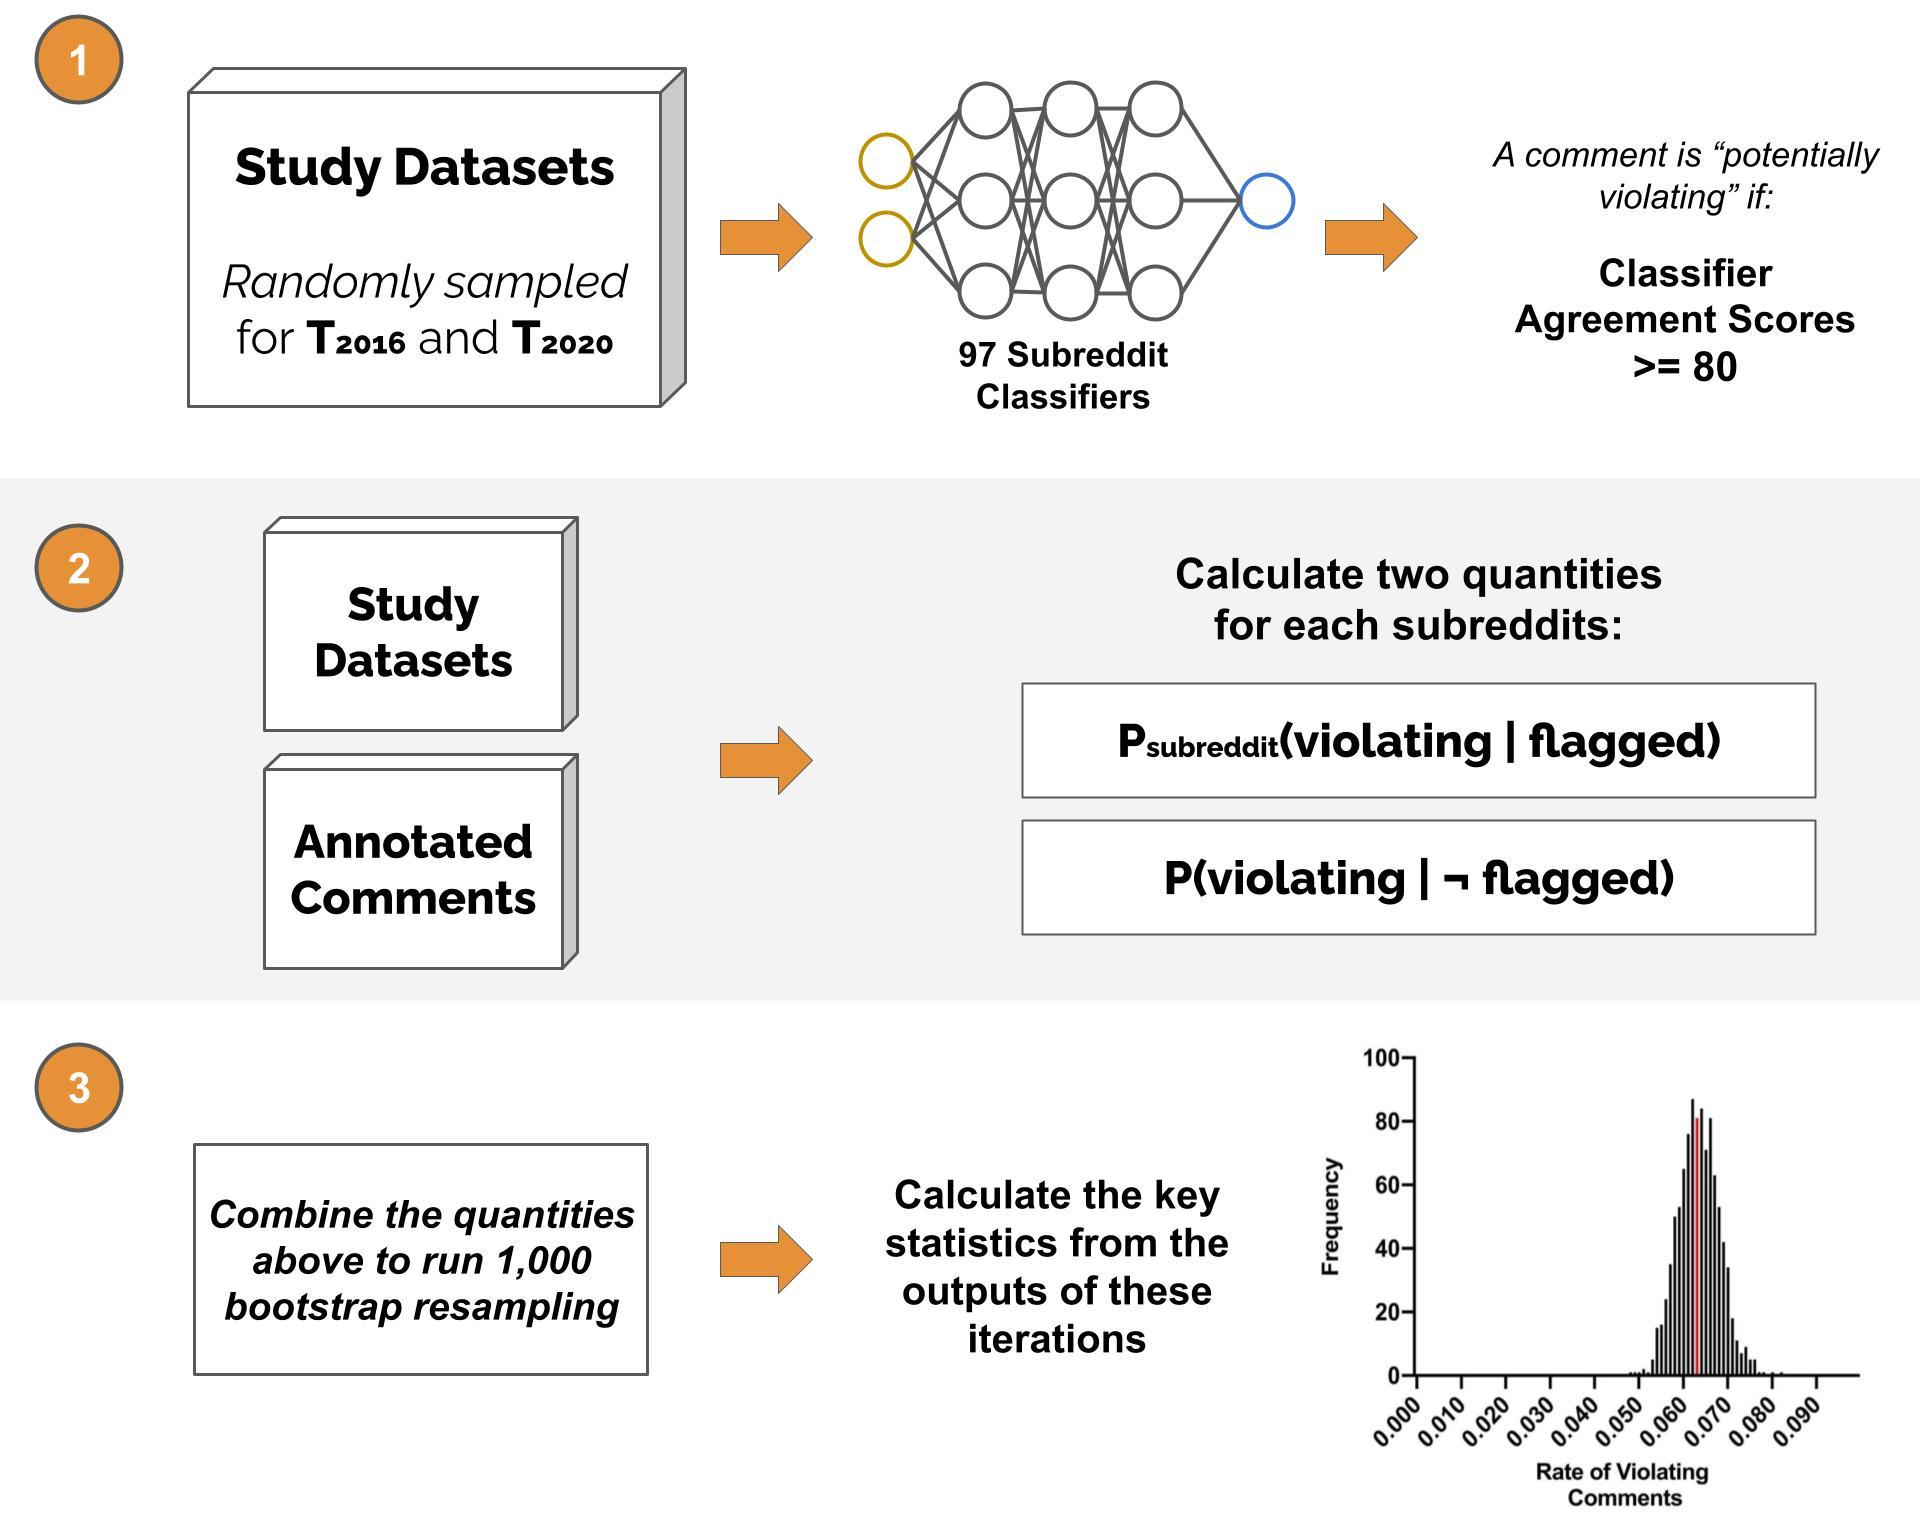
\includegraphics[width=1.0\textwidth]{content_minor_revision__Apr2022/images/bootstrap_workflow_6.jpg}
  \caption{\rnr{An overview of the sampling process in broad strokes. We start by randomly sampling unmoderated comments from $T_{2016}$ and $T_{2020}$ to generate our study datasets. We use these datasets and the annotated comments to calculate key quantities needed for our bootstrap resampling. We then combine these quantities to implement our resampling procedure, which we repeat 1,000 times for each time periods of our interest.}}
  \label{fig:bootstrap}
  \Description{Bootstrap resampling workflow}
\end{figure}


\subsection{\rnr{Bootstrapping Resampling Process}}
We took the following steps to sample our data for bootstrapping. For simplicity, we will describe our method with reference to the May 2016--March 2017 dataset, which we will refer to as $T_{2016}$. 

Intuitively, a bootstrap uses resampling with replacement to create a large number of parallel universes, each with the same number of comments as the original dataset, but each universe will have a slightly different number of norm violating comments due to the resampling with replacement. This variation across many parallel universes is what yields uncertainty confidence intervals on our estimates. However, each universe (bootstrap sample) must also contend with the fact that we have not manually annotated all 5 million comments in the dataset as violating or not. Rather than use a single fixed measurement of norm-violating comments per subreddit, which would ignore this source of uncertainty in the estimation, we resample our annotations over and over again with replacement to build in uncertainty due to our limited number of annotations. Figure~\ref{fig:bootstrap} provides an overview of this process, which is explained in detail below.

\subsubsection{\rnr{Study data and the flagged comments}} 
We began by randomly sampling a set of unmoderated comments. Specifically, we sampled 5,000 random comments from each of the study subreddits posted during this period dataset, for a total of 485,000 comments. These comments were sampled from the Pushshift Reddit corpus, which contains a complete capture of all comments on each subreddit. For clarity in presentation, we will call this sample of comments from 2016--2017, $T_{2016}$. We then ran all 97 subreddit classifiers on each of the sampled comments to calculate the classifier agreement score. Any comments that were flagged by at least 80 of the 97 classifiers as violating were labeled as \textit{flagged}.

\subsubsection{\rnr{Calculating intermediate probabilities}}
For the bootstrap, we needed to follow a procedure where we sample a comment, label it as flagged or not based on the classifiers, and then label flagged comments as violating or not based on human annotators. However, because we cannot tractably label every flagged comment in the bootstrap via human annotation, we relied on statistical generalization via the bootstrap. For this generalization to succeed, we require two empirically observed probabilities for each bootstrap iteration: $P_{subreddit}(violating \mid flagged)$, the true positive rate, the probability that a flagged comment in a particular subreddit is verified by annotators as an actual violation; $P(violating \mid \lnot flagged)$, the false negative rate, the probability that a comment that is not flagged as potentially violating via our classifiers is in fact violating according to our annotators.

\paragraph{$P_{subreddit}(violating \mid flagged)$.} The true positive rate, $P_{subreddit}(violating \mid flagged)$, carries uncertainty since we can only manually annotate a fixed number of comments per subreddit. To model this uncertainty, we re-estimate $P_{subreddit}(violating \mid flagged)$ with each bootstrap resample. Each iteration, for each subreddit, we take a random resample with replacement of the 32 flagged comments that annotators had labeled for each subreddit with each resample (e.g., sample 32 comments with replacement from the set of 32 flagged comments for the subreddit). This value of $P_{subreddit}(violating \mid flagged)$ is then used for that subreddit for that bootstrap iteration and varies with each iteration, capturing uncertainty in our estimate, and is used to help estimate whether a flagged comment in our sample is a true positive.

\paragraph{$P(violating \mid \lnot flagged)$.} Some comments that the classifiers do not believe to be macro norm violations will, in fact, be violations---and our bootstrap procedure must account for this so that it does not undercount the number of violations. To estimate the false negative rate, $P(violating \mid \lnot flagged)$, we use the sample of 1,000 \textit{non-flagged} unmoderated comments that we manually annotated in Section 3.4. These 1,000 comments showed a consistent 1\% false negative rate of our classifiers across 10 randomly chosen subreddits, so we treat this value as being consistent across all subreddits and do not parameterize it by subreddit. However, we still must model uncertainty in this estimate. So, for each bootstrap iteration, we resample 1,000 comments with replacement from the set of 1,000 comments and calculate $P(violating \mid \lnot flagged)$ as the proportion of comments that were not flagged as potentially violating but were in fact violating according to human annotators. We use this quantity to estimate whether a non-flagged comment in our sample is a false negative. As with the true positive rate, resampling with replacement will cause this value to vary from bootstrap iteration to iteration, critical to creating confidence intervals for our analysis.

\subsubsection{\rnr{Bootstrap resampling iteration procedure}}
These two probabilities enable our bootstrap procedure. In bootstrapping, we resample the dataset many times and measure the quantity of interest in each new instance. \rnr{In this study, we ran our bootstrapping procedure for 1,000 iterations (this is a typical number of iterations when conducting bootstrap resampling \cite{81_Bootstrap}). For each iteration, we resampled a number of comments that matched the complete number of comments on each of our study subreddits during our study period (i.e., 252,642,908 comments for $T_{2016}$). We also resample with replacement from the dataset of 5,000 classified comments each iteration, creating variation to model uncertainty in our sampling. Each bootstrap iteration also estimates new values for $P_{subreddit}(violating \mid flagged)$ and $P(violating \mid \lnot flagged)$ for each iteration, which combine to provide one datapoint in the final outcome distribution. In other words, each bootstrap sample creates an alternative universe of comments resampled from each subreddit, exhibiting natural variation in violation and moderation rates due to the random sampling.}

We illustrate this process with an example of bootstrap resampling the r/videos subreddit for $T_{2016}$. There were a total of 5,296,900 unmoderated comments that were on r/videos during $T_{2016}$. To populate each of these comments, we sampled a random comment from the subset of 5,000 random comments from r/videos that the classifiers had labeled. These 5,000 random comments had themselves been randomly sampled with replacement for this iteration of the bootstrap from the original set of 5,000 comments that were collected and classified. For r/videos, in one of the bootstrap samples, 1,249 of the 5,000 randomly sampled unmoderated comments (25\%) were flagged as potentially violating by the classifiers. If the sampled comment was flagged, then we randomly assign the comment as violating with probability $P_{r/videos}(violating \mid flagged)$ ($\approx 0.2$ in this bootstrap iteration) and attach the violation type(s) that human annotators tagged that comment with, and as not violating otherwise. If the sampled comment was not flagged, then we randomly assign the comment as violating with $P(violating \mid \lnot flagged)$ ($\approx 0.01$ in this iteration), and not violating otherwise. This process repeats to generate all 5,296,900 comments for r/videos.

We follow this process for all 97 subreddits, for all 1,000 bootstrap samples. The 1,000 samples provide a distribution and uncertainty estimate for the key statistics. Finally, through this process, we resample the same number of comments as the number of all unmoderated comments that were posted on these subreddits, some of which are labeled to be violating. So when we calculate the rate of unmoderated but violating comments in one bootstrap iteration, we add up the number of unmoderated but violating comments in each of the 97 subreddits and divide that by the number of all comments --- this gave us an estimation for r/videos, which was 5.95\% [2.16, 9.22] for $T_{2016}$, and 3.53\% [0.59, 9.14] for $T_{2020}$. This allows our bootstrap procedure to naturally take into account the different subreddit sizes --- through resampling more comments from the larger subreddits, the bootstrap will give more weight to the uncertainty on larger subreddits, in the analysis which are focused on the overall rates across the platform.

\subsubsection{2020 dataset}
As mentioned in the previous section, there are two periods of interest: one, from May 2016 to March 2017, the same period as when the moderated comments dataset $\mathcal{M}$ was collected, and the other from the last three weeks of December 2020, which we consider as a replication study on a slightly shorter but more recent timeframe. As we referred to the original dataset as $T_{2016}$, we will refer to the latter as $T_{2020}$. The process for $T_{2020}$ was identical to $T_{2016}$. Because $T_{2020}$ was a smaller dataset, however, its constituent samples were fewer in number. In particular, we \rnr{randomly} sampled 2,000 comments from each of the study subreddits instead of 5,000 commments, or fewer if the subreddit did not contain 2,000 comments during $T_{2020}$. This resulted in a total of 188,000 comments sampled and run through our 97 subreddit classifiers. Given the smaller sample size, the confidence intervals are wider for $T_{2020}$ than for $T_{2016}$.

\subsection{\rnr{Ablation Analysis with Fewer Annotations}}
Our bootstrap relies on a set of thousands of manually annotated comments from annotators. This gives rise to a possible threat to validity: that we did not manually annotate enough comments per subreddit to capture the uncertainty in the estimate per subreddit. To test whether this threat should be concerning, we performed an ablation analysis where we replicated our method using half of the manual annotations we had for each of the subreddits (that is, 16 annotations per subreddit instead of 32 for $T_{2016}$, and 4 per subreddit instead of 8 for $T_{2020}$). The main goal of this ablation analysis was to test how having fewer annotations impacts the uncertainty estimates of the bootstrap. Intuitively, as we have fewer and fewer samples, the confidence intervals will widen because if a rare event is sampled, it has a larger impact on the resulting estimate. We report our findings alongside our main results, in Section 6.

\section{CONCLUSION}
In this work, we aimed to quantify and characterize norm violating comments on a major online community platform. To accomplish this, we defined norm violating comments as those that would have been removed on most of the communities, and developed a human-AI pipeline for identifying such comments at scale. Finally, we employed bootstrap estimation to estimate the prevalence of these comments from two distinct periods: one from 2016 May--2017 March, and another during the final three weeks of December 2020. In doing so, our work presents a model pipeline that could serve as a point of reference to future work that tries to identify violating comments and provides empirical results estimating the prevalence of violating comments. Our findings suggest that despite the growing efforts to reduce harmful content in online social spaces, a large number of violating comments still populate these communities. Based on our findings, we highlight the need for continuous effort to improve our designs, policies, and moderation strategies.

\section{Measurements}
Using our pipeline for identifying violating comments and bootstrap sampling of comments, we estimated the dependent variables of interest. In this section, we present our specific measures that we derived from our method. 


\subsection{Estimating the Prevalence of Violating Comments}

\subsubsection{Overall prevalence} 
Our core dependent variable is the percentage of unmoderated comments that are \rnr{macro norm} violations. For each bootstrap sample, we calculated the percentage of violating comments. We then calculated our estimate as the median result across the 1,000 bootstrap samples, and calculated the 95\% confidence interval across those samples. 

\subsubsection{Prevalence per subreddit} 
Do some subreddits contain a higher rate of macro norm violating comments than the others, and if so, why? To answer this question, we estimated the percentage of violating comments for each of the subreddits across each of the bootstrap samples, and again calculated the median and 95\% confidence interval per subreddit. Given that the $T_{2020}$ sample, as mentioned previously, is a smaller scale replication of the $T_{2016}$ sample, we found that there is not enough data to draw statistically meaningful results for each of the subreddits for $T_{2020}$. Therefore, we focused our analysis in this particular subsection on the $T_{2016}$ sample. 

We tested the factors that were associated with a subreddit having a higher count of violations. We started by taking the sampling approach as we did above to estimate the count of violating comments for each of the study subreddits. We hypothesized that two relevant predictive variables might influence the rate of violating comments: 1) the topic of a given subreddit and 2) the ratio of the number of moderators to the number of comments. Our focus on the first variable was motivated by our observation that some communities might be more prone to hosting macro norm violations that are topically relevant (e.g., politically inflammatory comments for political subreddits or pornography for NSFW subreddits), while our focus on the second variable was informed by prior work suggesting that moderators in subreddit communities are overloaded and unable to review every comment posted~\cite{Chandrasekharan2018internet, 18_Gilbert}.

To test these hypotheses, we first collected the relevant data for these variables. To get the respective topics for our study subreddits, we matched the study subreddits to categories on r/ListOfSubreddits’ thematically organized list of subreddits.\footnote{\url{https://www.reddit.com/r/ListOfSubreddits/wiki/listofsubreddits}} The list contains multiple layers of thematic hierarchy. From this, we picked the second-highest thematic layer (e.g. r/AskReddit was categorized as “Discussion,” and r/Pokemon as “Entertainment”) for our subreddits as the top layer was too broad to be meaningful. This resulted in eleven mutually exclusive topic categories for our 97 study subreddits.  We then manually collected the number of moderators who were present in October 2016 (the middle of the 11-month period when $\mathcal{M}$ was collected) for each of the subreddits by using the Wayback Machine to access an archived version of each subreddit's homepage on October 1st, 2016, or the earliest subsequent date when the page was crawled. We then calculated the ratio of moderators to comments for each of the subreddits. Finally, we retrieved the number of all comments (including those that were removed by the users or moderators) that were posted on each of the 97 study subreddits from $T_{2016}$ -- we used this information as the offset to our Poisson model described below. To address the non-normal distribution of the number of comments and moderator-to-comment ratio in our regression, we log transformed these variables.

We then employed a Poisson regression \cite{63_poisson} to model the rate of macro norm violating comments in a given subreddit using the three aforementioned predictive variables as our independent variables. \rnr{Poisson regression was an appropriate choice because it is designed to model rate data. We followed a common practice of setting an offset---in our case, the size of the subreddit in terms of the number of comments--- to the Poisson regression model to make it appropriate for rate data \cite{94_Anderson, 95_Gardner}.} For better interpretability of our model, we treated the ``general content'' topic category as the baseline of the indicator (dummy) variable for topic. Finally, to interpret our results, we exponentiated the variable coefficients in our model to calculate the incidence rate ratios. For instance, as we will cover in the next section, \rnr{the number of moderators to comments ratio in a subreddit is a significant predictor of the rate of violating comments in a subreddit (p<0.001) where for every unit increase in the log-transformed number of comments in a subreddit, the rate of violating comments is expected to increase by a factor of 2.07 (=$e^{0.728}$).}


\subsection{Determining the Characteristics of Violating Comments}

\subsubsection{Prevalence by violation category} 
So far, we defined a comment to be violating if it violates one of the macro norms of Reddit. But here, we describe our analysis that takes a closer look at the variance in the prevalence of different macro norm violations and the rate at which they occur. In order to better understand the prevalence of each of the macro norm violations among the unmoderated comments, \rnr{we measure the percentage of sampled violations that fall into each of the violation categories}. Specifically, we take the average number of norm violations per category that across the study subreddits in each bootstrap iteration, and as before, report the median and confidence interval across the 1,000 bootstrap iterations.

Are all categories of macro norm violations removed by the moderators at the same rate? To answer this question, we \rnr{take the following steps to} estimate the number of all comments (moderated and those still online) that violate each specific one of the macro norms. To estimate the number of violations for each of the macro norms within the moderated comments, we require a complete set of all moderated comments from our study subreddits, which we gathered earlier as $\mathcal{M}$ for $T_{2016}$. To extend $\mathcal{M}$ to $T_{2020}$, we reimplemented the original high-frequency scraping process used in prior work to generate $\mathcal{M}$ for $T_{2016}$~\cite{Chandrasekharan2018internet}. We then randomly sampled from $\mathcal{M}$ (N=776 comments for the longer $T_{2016}$ period; N=188 for the shorter $T_{2020}$ period). We then followed the same human annotation process from Section~\ref{sec:annotation} to annotate each moderated comment with any macro norms that it violated. Using this, we calculated the estimated number of comments that violate each of the macro norms within the moderated comments dataset. We combined this with the estimated number of unmoderated violations for each macro norm to estimate the overall number of violations for each of the macro norms considering both moderated and unmoderated comments combined. With this number of violations, we then proceeded to calculate the rate at which each of the macro norms are moderated.

\subsubsection{Comparing the rate of engagement} 
Reddit comments accrue engagement over time in the form of upvotes, downvotes, and replies. The “score” of a comment is determined by subtracting the number of downvotes from the number of upvotes the comment gained over time, and “replies” are comments that respond to the given comment in the thread. Score is a useful dependent variable to track because it is a strong determinant of how high in the thread the comment sits.\footnote {On Reddit, users can choose one of the three options -- top, hot, and best -- for determining what comments should come at the top. Top is simply whichever comment has the highest score, hot is the log-transformed absolute value of the score with extra weights for the age of the content, and best is the number of upvotes divided by the number of downvotes. See \url{https://www.reddit.com/r/explainlikeimfive/comments/1u0q4s/eli5_difference_between_best_hot_and_top_on_reddit/}} The number of top-level replies can serve as a proxy for measuring whether the given comment generated, or ended, a discussion.\footnote{The Perspective model from Jigsaw for measuring toxicity used human annotations to train where a comment was asked to be annotated if it were “rude, disrespectful, or unreasonable… that is likely to make you leave a discussion” \cite{60_Perspective}.}
We explored whether the violating comments result in significantly higher or lower scores, and whether they receive more or fewer “top-level replies” (replies that directly respond to the given comment in the thread of replies). To investigate this, we compared the scores and the number of top-level replies that the unmoderated violating comments got to the global average number of online comments the study subreddits in our $T_{2016}$ and $T_{2020}$ samples.


\subsubsection{Comparing language usage} 
Does the way in which a macro norm is violated impact its likelihood of remaining on the site or being moderated? We compared the writing style of moderated comments vs. unmoderated violating comments on two dimensions: readability and emotionality. For measuring readability of a comment, we used the Flesch–Kincaid readability test~\cite{64-kinkaid} to retrieve the comment’s readability score, where a higher score indicates that the comment is easier to read. For measuring emotionality of a comment, we used Evaluative Lexicon 2.0~\cite{65_Rocklage, 66_Rocklage}, an imputation-based dictionary that assigns an emotionality score to text where higher score means that the comment is more likely to trigger an emotional reaction rather than a cognitive response that reflects a person’s beliefs about the topic of discussion \cite{66_Rocklage}.


\begin{figure}[tb]
  \centering
  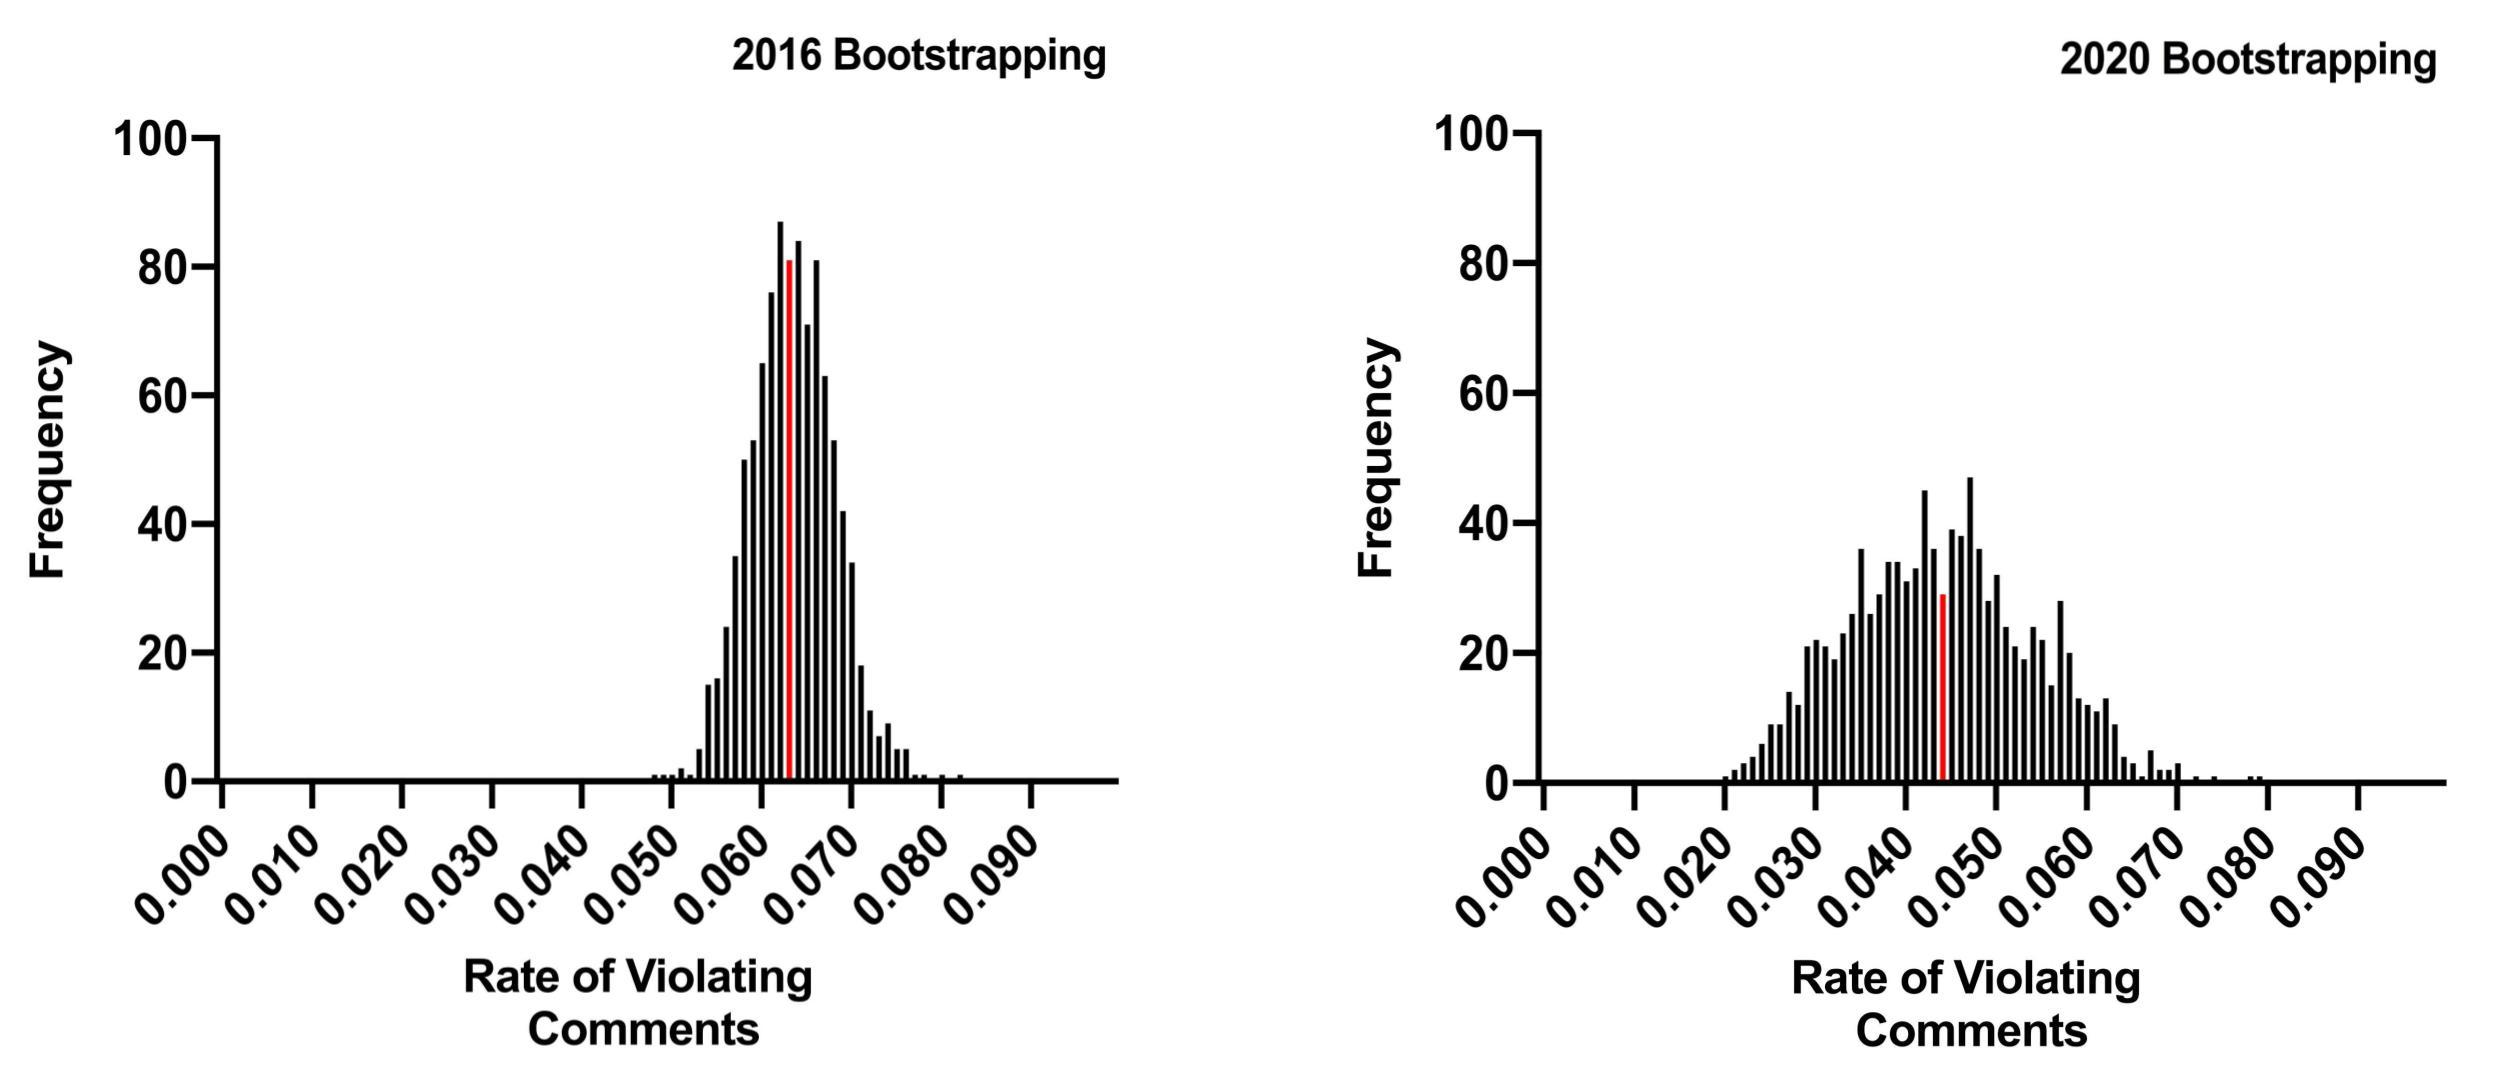
\includegraphics[width=0.95\textwidth]{content_minor_revision__Apr2022/images/bootstrap_rate.jpg}
  \caption{The results of our bootstrap sampling. The figures show the overall rates of violating comments that are left unmoderated for all 1,000 simulations of Reddit for $T_{2016}$ and $T_{2020}$. The 50th percentile rates for the 1,000 bootstrap samples are colored red for the two periods.}
  \label{fig:bootstraprate}
  \Description{Annotation Interface}
\end{figure}
 
\begin{figure}[tb]
  \centering
  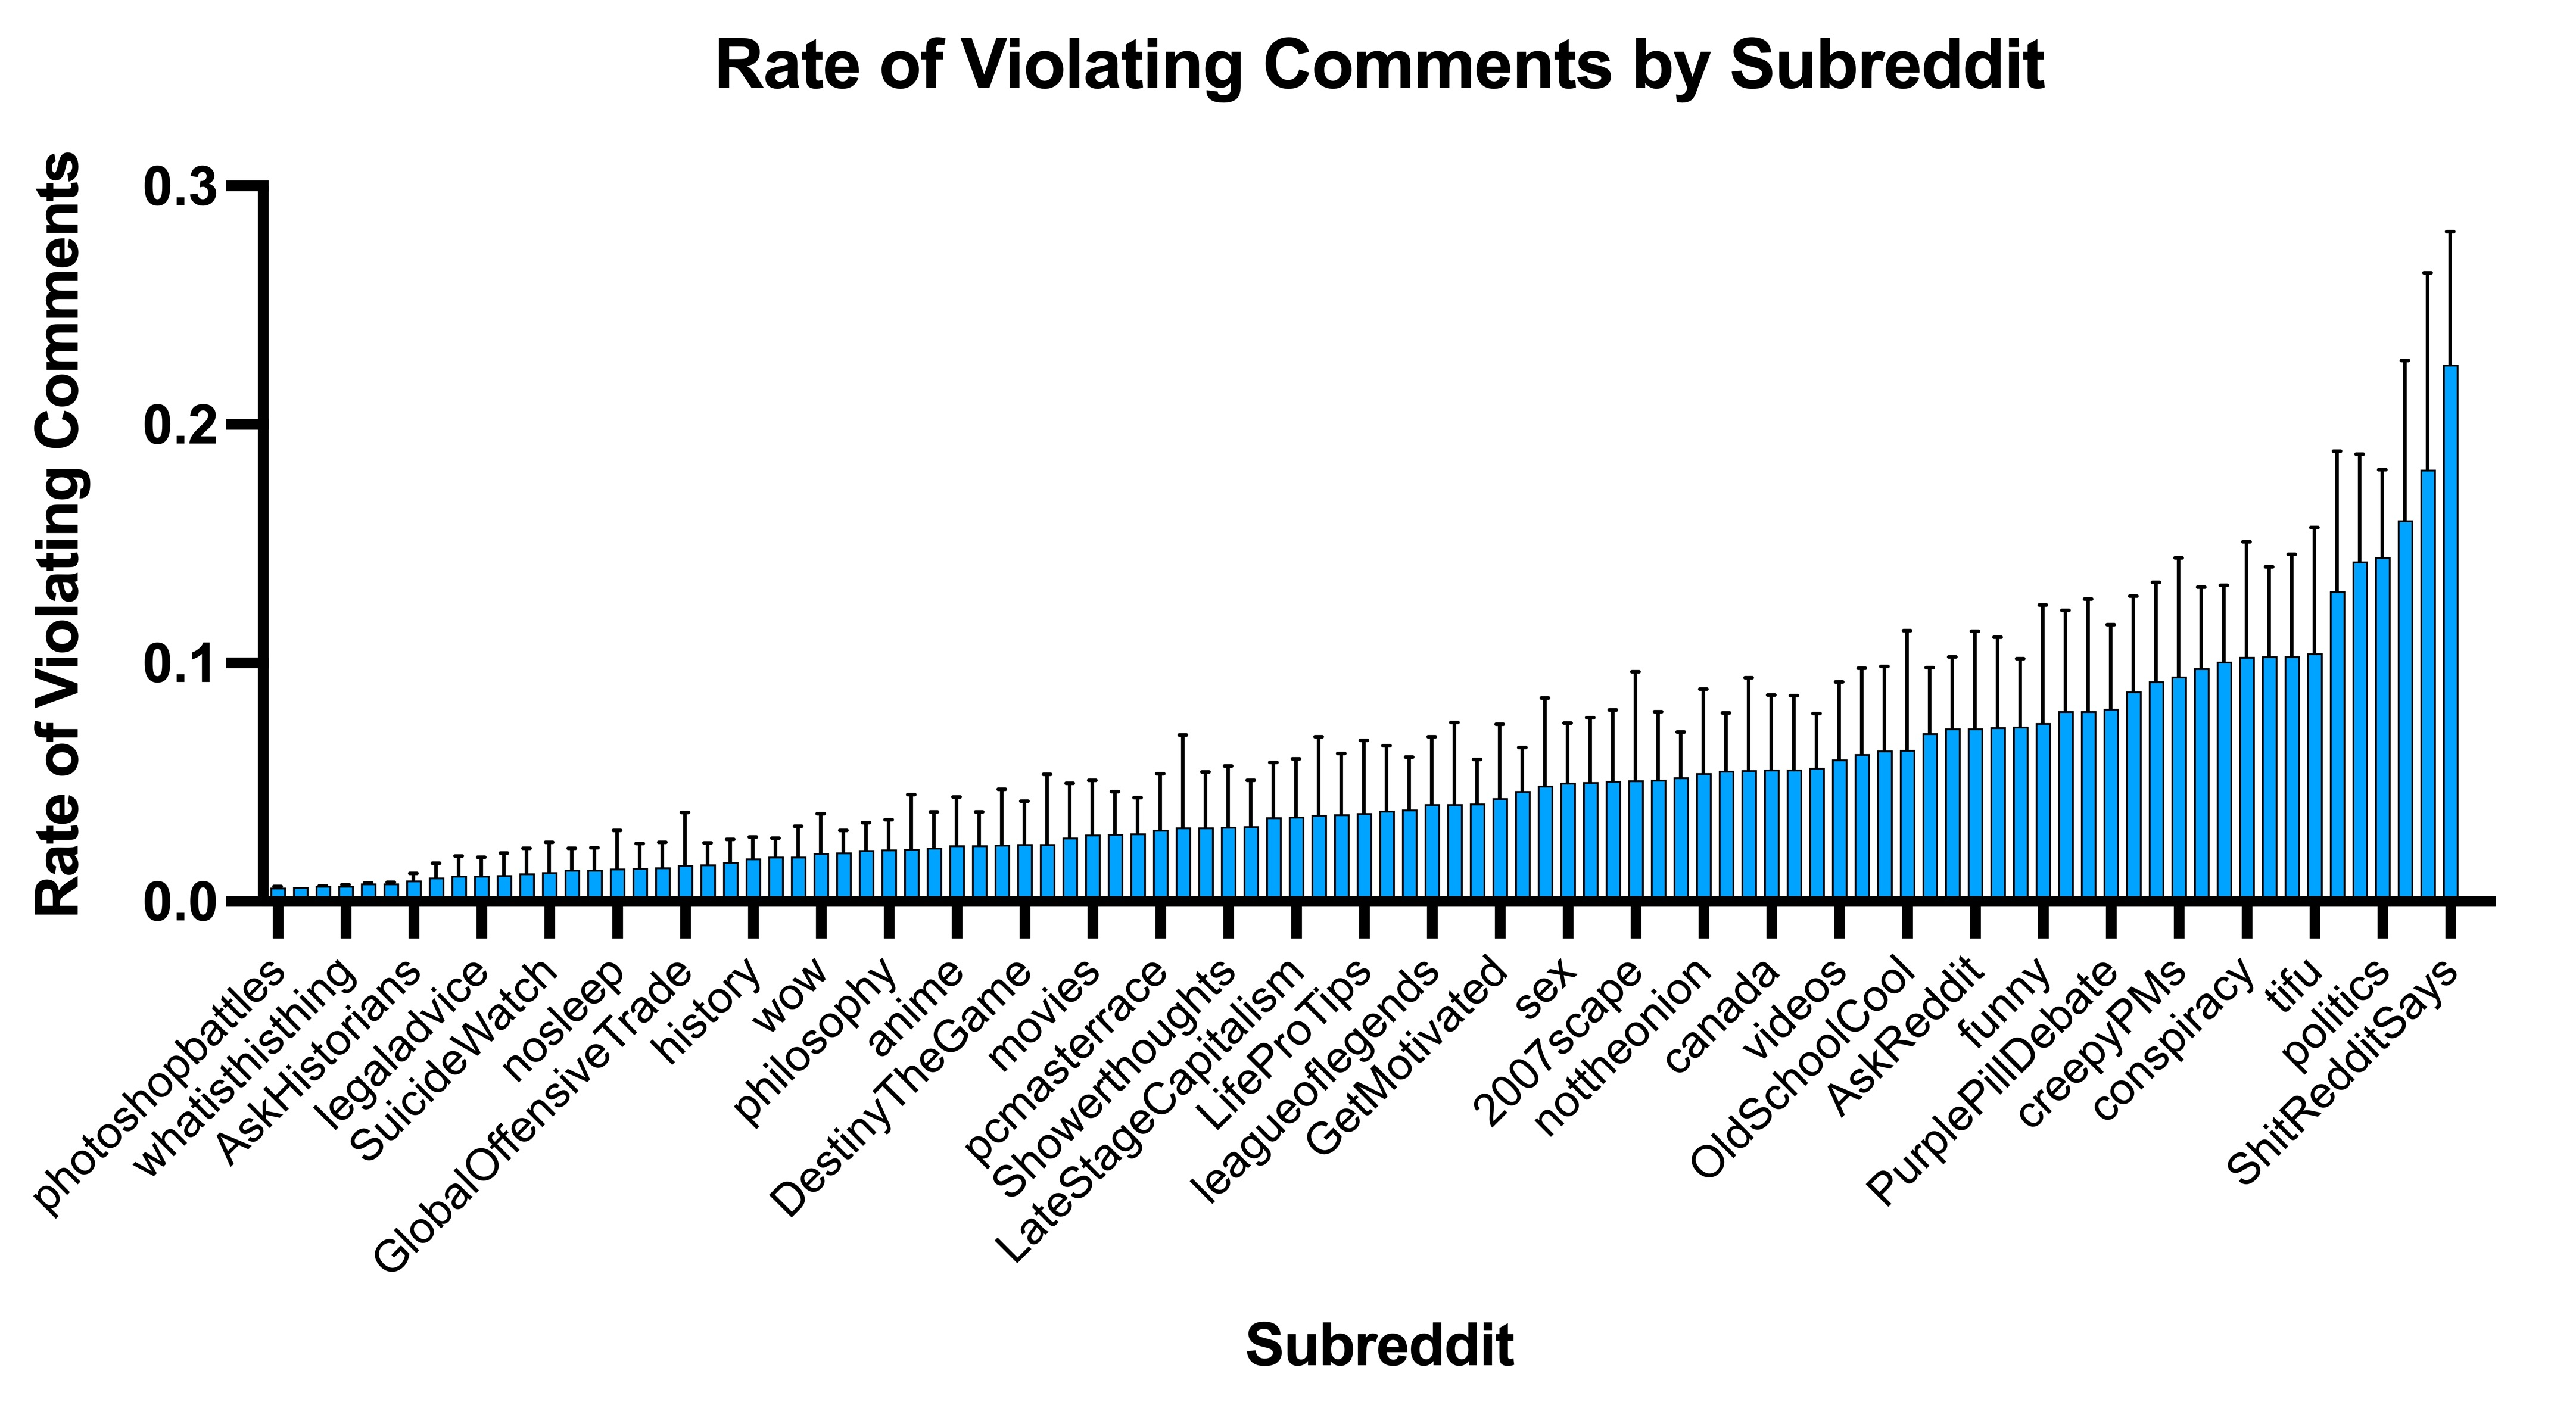
\includegraphics[width=0.95\textwidth]{content_minor_revision__Apr2022/images/all_rate_of_violating.jpg}
  \caption{Rate of \rnr{macro norm} violating comments by subreddit in $T_{2016}$. The lighter lines indicate 95\% confidence intervals. Subreddits vary in levels of violating content; some subreddits like r/depression (1.10\%) and r/Android (1.42\%) contain almost no  \rnr{violating} comments online, whereas some like r/creepyPMs (9.42\%) and r/EnoughTrumpSpam (14.27\%) contains much higher rates of \rnr{violating} comments.}
  \Description{Rate of macro norm violating comments by subreddits}
\end{figure}


\section{RESULTS}

In this section, we present the results of our analyses. We start by reporting on the prevalence of violating comments across our study subreddits and then describe their characteristics in terms of their content, rate of engagement, and language usage.

\subsection{Prevalence of Violating Comments}

\subsubsection{Macro norm violating comments are common}
Figure~\ref{fig:bootstraprate} reports the rate of macronorm violating comments across our 1,000 bootstrap iterations. In $T_{2016}$, 6.25\% (95\% CI [5.36\%, 7.13\%]) of all unmoderated comments are violations. In $T_{2020}$, 4.28\% (95\% CI [2.50\%, 6.26\%]) of all unmoderated comments are violations. \rnr{There are fewer macro norm violating comments over time: a permutation test confirms that the rate of macro norm violating comments is lower in $T_{2020}$ than $T_{2016}$ ($p<.001$).} 

\subsubsection{\rnr{Ablation analysis of the bootstrap confidence intervals}} 
\rnr{In order to (1) confirm that our bootstrapping procedure widens its confidence intervals as fewer human annotations are available, as it should, and (2) confirm that our current number of annotations is sufficient for our estimation goal, we tested the width of the bootstrap's confidence intervals as we ablated to half the number of human annotations per subreddit. On our full dataset for $T_{2016}$ with 32 human annotations per subreddit, the 95\% confidence interval's width is 1.77\%. When we ablate and halve the number of labels from 32 to 16 per subreddit, the confidence interval's width becomes $T_{2016}$ becomes  2.58\% ([4.60, 7.18], median 5.90\%), a 95\% CI width that is .8\% larger. For our smaller $T_{2020}$ dataset with 8 annotations per subreddit, the 95\% CI width is 3.76\% ([2.50, 6.26]). Here, when we ablate and halve the number of labels from 8 to 4 per subreddit, the 95\% CI width widens to 5.43\% ([1.96, 7.39], median 4.27\%), or 1.67\% wider than the original estimate.}


% \usepackage{booktabs}




\begin{table}[tb]
\centering
\captionof{table}{The results of Poisson regression that predicts the rate of problematic comments in a subreddit. We find that the number of comments in a subreddit, as well as a few of the topic categories are strong predictors of the rate of problematic comments a subreddit may have. The topic "general content", which was included in the model, is not shown as it was used as the baseline dummy variable for the categorical variable.}
\begin{tabular}{lllll} 
\toprule
                               & \textbf{Coefficient} & \textbf{SE} & \textbf{z-score} & \textbf{p-value}  \\ 
\toprule
Intercept                      & -5.919               & 1.249       & -4.740           & < 0.001 (***)      \\
log(mod to comment ratio)      & -0.728               & 0.244       & -2.986           & 0.003 (**)        \\
Topic: Hobbies and Occupations & -2.048               & 0.280       & -7.304           & < 0.001 (***)      \\
Topic: NSFW                    & 1.958                & 0.253       & 7.742            & < 0.001 (***)      \\
Topic: Discussion              & -1.021               & 0.421       & -2.423           & 0.015 (*)         \\
Topic: Politics                & 0.628                & 0.260       & 2.414            & 0.016 (*)         \\
Topic: Humor                   & 0.408                & 0.251       & 1.621            & 0.105             \\
Topic: Lifestyle               & 0.0879               & 0.321       & 0.271            & 0.787             \\
Topic: Educational             & -1.191               & 0.647       & -1.840           & 0.078             \\
Topic: Entertainment           & -0.165               & 0.285       & -0.579           & 0.563             \\
Topic: Technology              & -0.387               & 0.325       & -1.191           & 0.233             \\
Topic: Other                   & 0.692                & 0.324       & 2.135            & 0.033             \\
\bottomrule
\end{tabular}
\end{table}



\rnr{Two observations fall out of this ablation analysis. First, we observe that the width of the confidence interval widens as we have fewer annotated comments per subreddit: from 1.77\% with 32 annotations to 2.58\% with 16 annotations in 2016, and from 3.76\% with 8 annotations to 5.43\% with 4 annotations in 2020. This confirms that bootstrapping is not producing overconfident confidence intervals: the confidence intervals widen as we have fewer and fewer labels. Second, we observe that, for 2016 in particular, 32 labels is far more than necessary for the confidence interval to be tight: the interval does not begin to dissolve until having only four labels per subreddit, and providing more than 32 labels per subreddit will not substantially reduce the width of the confidence interval further. The reason for this stability is that, while the estimate for any particular subreddit may be more uncertain, aggregating over nearly 100 subreddits substantially reduces the overall uncertainty.}



\subsubsection{\rnr{Topic and moderator ratio predict the rate of macronorm violations}}
In this subsection, we focus our efforts on the $T_{2016}$ sample. The rate of \rnr{macro norm} violating comments for individual subreddits averages 4.9\% (std=4.0\%), but there is a large spread across different subreddits (Figure 5). For example, subreddits such as r/AskHistorians (0.90\%; 95\% CI [0.73\%, 1.12\%]) and r/science (1.10\%; 95\% CI [0.70\%, 1.61\%]) had lower rates of macro norm violating comments than ones such as r/atheism (10.06\%; 95\% CI [6.99\%, 13.27\%]) and r/politics (14.46\%; 95\% CI [10.79\%, 18.12\%]). Our Poisson regression model, summarized in Table 3, suggests that these differences are associated with the subreddit's topic and its moderator to comment ratio. More specifically, subreddits on NSFW (p<0.001) or political (p=0.016) topics have higher a rate of violating comments, and those hosting hobbies and occupation topics (p=0.001), or discussion topics (p=0.018) are associated with fewer violating comments. Additionally, higher moderator-to-comment ratios are associated with fewer violating comments (p=0.003). 

Although NSFW and political topics featured a higher rate of macro norm violating comments, this did not mean that subreddits covering topics other than these two necessarily had a small number of macro norm violating comments. When excluding 17 subreddits whose topics were categorized as either NSFW and political, we find that the remaining subreddits still had violating comments at the rate of 5.26\% (95\% CI [4.27\%, 6.39\%]). 



\begin{figure}[tb]
  \centering
  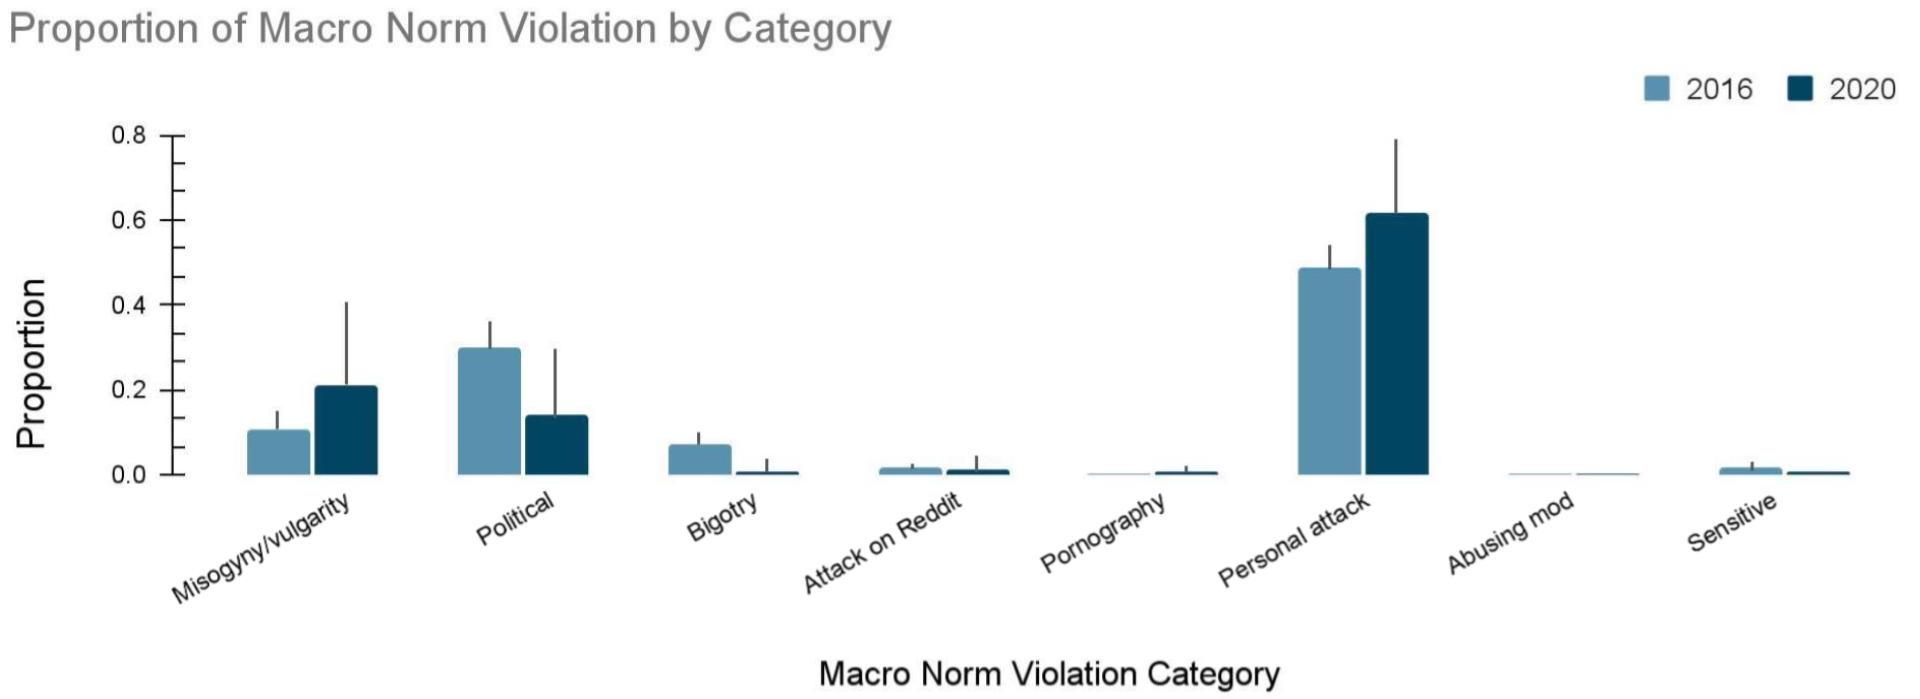
\includegraphics[width=1\textwidth]{content_minor_revision__Apr2022/images/macro_norm_violation_fixed_2.jpg}
  \caption{The proportion of macro norm violation by the eight categories among the unmoderated problematic comments according to our annotators. In $T_{2016}$ as well as $T_{2020}$, personal attacks were the most common macro norm violations. Politically inflammatory comments, on the other hand, have become less prevalent.}
  \Description{Proportion of Macro Norm Violation by Categories}
\end{figure}
% THIS HAS TO BE WITH 6.2.1


\subsection{Characteristics of Violating Comments}
In this subsection, we delve deeper into the violating comments to explicate the categories of violation, engagement rate, and language usage. 



\subsubsection{Personal attacks are the most prevalent category of violation.} 
The eight macronorms are not equally prevalent (Figure 6). In $T_{2016}$, personal attacks (48.58\%; 95\% CI [40.66\%, 56.66\%]) and politically inflammatory comments (30.16\%; 95\% CI [22.80\%, 37.54\%]) are particularly prevalent macronorm violations. On the other hand, categories such as posting pornographic links (<1\%) or abusing moderators (<1\%) were less common. Similarly, in $T_{2020}$, personal attacks (61.94\%; 95\% CI [45.06\%, 80.40\%]) remain the most prevalent, misogyny/vulgarity violations have become more prevalent (20.90\%; 95\% CI [1.33\%, 40.67\%]), and politically inflammatory comments have become less common (14.19\%; 95\% CI [4.49\%, 30.37\%]). 



\subsubsection{Macronorms are moderated at different rates} Moderation removed 4.86\% of macronorm violating comments in 2016–2017, and 10.54\% in 2020. Not all types of macro norm violations were moderated at the same rate, however.
In $T_{2016}$, comments that include links to pornography were moderated at the highest rate (34.53\%), followed by those that abuse or criticize moderators (26.17\%) and those that accuse another of being sensitive (12.87\%). On the other hand, politically inflammatory comments (4.30\%) and misogyny/vulgarity (4.13\%) were less likely to be moderated. Some trends still held in $T_{2020}$, where comments that include pornography were moderated at the highest rate (45.04\%). Nearly all categories were more heavily moderated in 2020 than in 2016.
We summarize the results in Figure 7. 


\subsubsection{Violating comments get fewer upvotes}
We find that in $T_{2016}$, \rnr{macro norm} violating comments garnered an average score of 7.32 (std=21.97), which is significantly lower than the global average of 10.27 (std=95.95) in our dataset according to Welch's t-test (t(469647) = -3.29, p = .001). However, there was no significant difference in the number of top-level replies; the violating comments got 2.00 top-level replies (std=9.25), vs. the global average of 1.92 (std=7.32): t(469647) = 0.21, p=0.83. These result replicate in the $T_{2020}$ sample; the comments that were annotated as violating got an average of 6.07 upvotes (std=13.09), which is significantly lower than the global average of 12.17 (std=119.94) that our sample of 188,000 comments got (t(415515) = -4.30, p < .001). Similarly, there was no significant difference in the number of top-level replies; the violating comments got 1.77 top-level replies (std=2.81) where  1.77 (std=6.82) was the global average (t(415515) = -0.003, p=0.99).


\begin{figure}[tb]
  \centering
  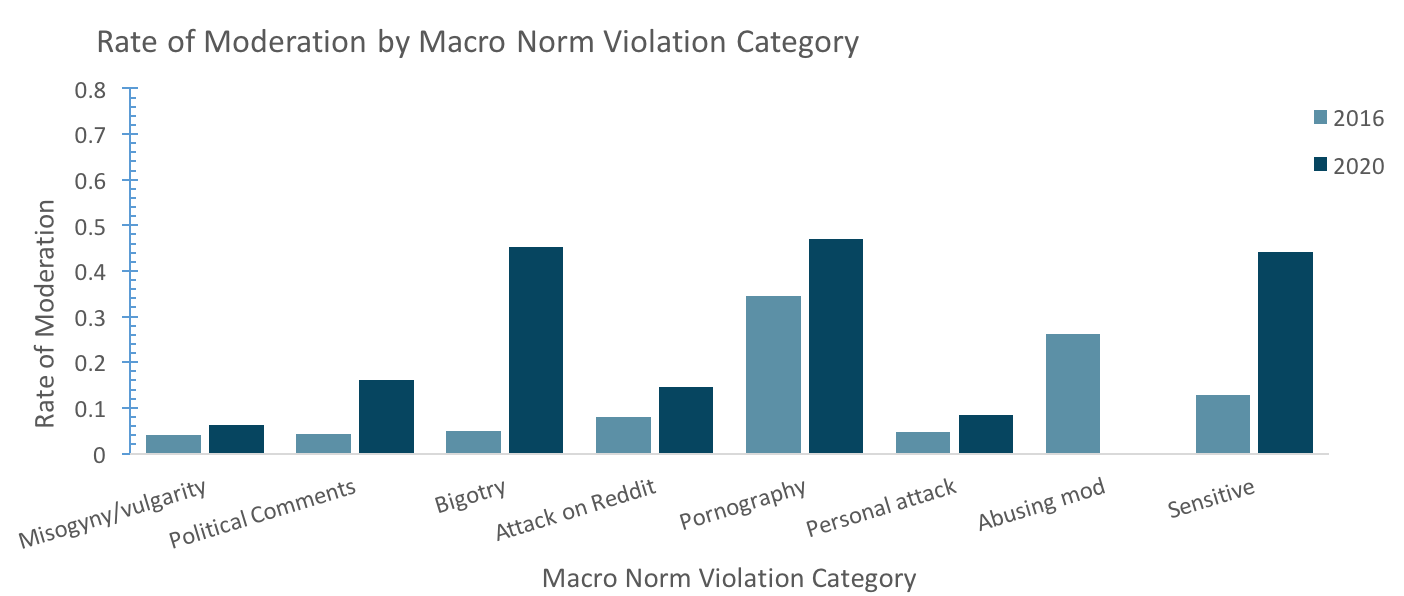
\includegraphics[width=1\textwidth]{content_minor_revision__Apr2022/images/ef_MODERATION.png}
  \caption{The rate of moderation by the eight macro norm violation categories acquired through stratified sampling. In $T_{2016}$, comments that contain links to pornography and comments that abuse or criticize moderators were moderated at the highest rate. In $T_{2020}$, comments with links to pornography is still among the most commonly moderated categories of norm violation. In addition, the overall rate of moderation has increased.  }
  \Description{Rate of moderation by macro norm violation categories}
\end{figure}
% THIS HAS TO BE WITH 6.2.2. AND COME AFTER PROPORTION... 




\subsubsection{More readable and emotional comments are more likely to remain unmoderated} We find that in $T_{2016}$, the readability scores of unmoderated macro norm violating comments averages 62.38 (std=122.51) while the scores of moderated comments averages 33.59 (std=1849.25). Additionally, using Welch's t-test, we confirm that the difference in readability between these two groups of comments is significant (t(2007616)=5.62, p<0.001), indicating that the unmoderated macro norm violating comments are easier to read than the moderated comments. This is replicated in $T_{2020}$, in which the readability scores of the unmoderated macro norm violating comments averages 76.95 (std=31.94) while the scores of moderated comments averages 64.35 (std=293.49). Additionally, this difference between the two groups remains significant (t(160481)=3.59, p<0.001). 

Similarly, we find that in $T_{2016}$, the average emotionality scores of unmoderated macro norm violating comments averages 5.14 (std=1.30) while those of moderated comments averages 0.74 (std=0.51). Once again, the difference in terms of the emotionality score between these two groups of comments is significant according to Welch's t-test (t(378432)=59.89, p<0.001), indicating that the unmoderated macro norm violating comments are more emotional than the moderated comments. This is replicated in $T_{2020}$ in which the average emotionality scores of unmoderated macro norm violating comments averages 4.75 (std=1.40) while those of moderated comments averages 0.80 (std=0.49) with the difference between the two groups being significant (t(74126)=40.90, p<0.001). 



\section{Related Work}
In this section, we cover prior work in characterizing and identifing anti-social behavior in online communities. Despite the continued effort to identify harmful content online, the existing approaches face significant methodological challenges. This presents a fertile ground in which empirical results highlighting what today's content moderation fails to capture could provide value in guiding the future effort in content moderation.

\subsection{Anti-social behavior in online communities}
Anti-social behavior has been documented for essentially as long as online communities have been documented~\cite{Dibbell1993rape}. A review of the causes of, and responses to, such behavior, is the focus of~\citeauthor{kiesler2012regulating}~\cite{kiesler2012regulating}. One form of anti-social behavior is trolling, which is typically defined as intentional disruption of the community. Trolling is sometimes attributed to the online disinhibition effect~\cite{suler2004online}, where we engage in behavior online that we might not in face-to-face interaction. There exists a set of individuals who are dispositionally oriented toward troll behavior~\cite{buckels2014trolls}, and engage in anti-social behavior because they are redirecting internal feelings~\cite{varjas2010high} or do it for fun~\cite{shachaf2010beyond}. While such individuals are equally uncivil both online and online, they have more reach and visibility online~\cite{bor_petersen_2021}.

Another form of anti-social behavior is non-premediated, often referred to as flaming~\cite{83_Kayany,Kiesler1984social}. Evidence suggests that many online users can be tipped into engaging in flaming through a combination of mood and environmental signals~\cite{cheng2017anyone}. Human observers can predict with reasonable accuracy whether a discussion thread is going to end with hostility~\cite{zhang2018conversations}, but we are poor at estimating how others will react to our own comments~\cite{chang2020don}.

Facebook answered the increasing pressure related to hate speech on its platform with a brief transparency report suggesting, for the first time, that roughly 1 in 1,000 content views on its platform include what the platform considers to be hate speech \cite{58_Culliford}. Similarly, Reddit's Safety Team announced the impact of a certain form of moderation like banning of a toxic community on curbing toxic content \cite{78_Vincent} while YouTube provided a summary of the type of content the platform is trying to remove \cite{77_YoutubeTeam}.

Measuring the prevalence of these behaviors remains an open challenge. One thread of prior work has used survey methods to understand the prevalance of anti-social behaviors online (e.g.,~\cite{pew_harassment_results,vitak_harassment}). Another thread has used log data to observe when content is flagged or removed (e.g.,~\cite{cheng2017anyone,twitch_transparency_report}). The present research extends these efforts through directly sampling and coding online behaviors as violations. Such an approach allows us to avoid sampling and reporting biases, though it makes tradeoffs to do so. For example, not all violations are created equal, and survey methods will be better at capturing the impact of seeing a violation.


\subsection{Moderation}
Content moderation is a common response to anti-social behaviors. Content moderation strategies can be broadly categorized into human moderation and automated moderation. Where online forums and discussion boards were previously managed in large part by human moderators who would carefully sift through the content posted and remove those that go against a given community's standard \cite{27_Lampe}, online social media companies today are increasingly relying on automated tools to scale up the moderation effort \cite{28_Gorwa, 29_Roberts}. But despite the ongoing efforts to improve these strategies, both human moderation and automated moderation face challenges.

\subsubsection{Human Content Moderators}
Online content moderation strategies that rely on human moderators to control anti-social content involve dedicated moderators to manually inspect and act on such content. Although human moderators can often make more nuanced decisions than automated moderators by taking into consideration the context \cite{28_Gorwa, 30_MSB, 31_Lessig, alkhatib2019street} and ``behind-the-scenes'' norms of a local community that are less explicit \cite{Chandrasekharan2018internet}, they face significant challenges in ensuring that all content is reviewed in modern-day social media platforms where participants number in hundreds of millions to even billions \cite{32_Preece, 33_Williams}. Therefore, human moderators often take a reactive instead of a proactive approach in which the content that users share is first posted online and then reviewed once they have been flagged by others as anti-social \cite{9_Roberts, 34_Gillespie}. This results in anti-social content remaining visible to the users within the online community until it is reviewed by a moderator, or in the worst case, remain unaddressed indefinitely \cite{34_Gillespie}. 

% In recent years, large social media companies such as Facebook, Twitter, and YouTube have hired external human moderators to scale up such moderation processes \cite{35_Seering}. However, such partnering has drawn critiques not only because these external human moderators are continuously exposed to highly violent and inappropriate content for low wages \cite{chandrasekharan2019crossmod}, but also because they are dispersed globally and might not be familiar with social norms or culturally sensitive racist, homophobic, and misogynistic tropes within the country where the content originates from \cite{36_Stecklow, 37_Chen, 38_Wray}.
 
\subsubsection{Automated Content Moderators}
To moderate the large volume of content that is shared on social media platforms, \rnr{there has been an increasing effort to create tools that can automatically identify and act on anti-social behavior \cite{39_Bickert, 40_Google, 41_Twitter, 92_Chandrasekharan}}. \rnr{Such tools range from simple word or source-ban lists that filter content based on block-listed words, URLs, and source IP addresses \cite{42_HN}, to more sophisticated AI tools that leverage machine learning and natural language processing techniques \cite{chandrasekharan2019crossmod, 93_Chancellor}}. \rnr{Particularly within the context of self-governed online communities, recent academic research has tried to both better understand what the online communities value and consider to be norm violating content that should be removed \cite{Chandrasekharan2018internet, 35_Seering}, and build tools and datasets that would help these communities implement automated ways for identifying and flagging the norm violating content~\cite{1_Chandrasekharan, chandrasekharan2019crossmod, 93_Chancellor}.}

And concurrent with the research that showed automated tools could be useful for efficiently capturing textual cyberbullying \cite{43_Dinakar, 44_Xu}, vulgarity and other anti-social behaviors online \cite{4_Chancellor, 1_Chandrasekharan, 5_Cheng}, large social media platforms started to transition their moderation strategy to be more reliant on automated tools \cite{35_Seering, 45_Geiger}. For example, following a major public controversy in which Facebook reportedly became the medium for hate speech that incited genocide against the Muslim population in Myanmar, the social media platform improved its Burmese hate speech classifier to increase automated takedowns of content by 39\% \cite{46_GIFCT}. Meanwhile, YouTube reports that 93\% of the videos on its platform that are removed for violent extremism are flagged by machine-learning algorithms \cite{40_Google}, while Reddit’s subcommunities now routinely employ AutoModerator to automatically filter out comments violating the community standards \cite{47_reddit}.

However, the automated tools for fighting anti-social content online have received criticism for their limitations. One of the most commonly cited limitations includes automated moderation tools’ inability to take into consideration the context in which an online conversation is taking place \cite{30_MSB, 31_Lessig, 48_Pater}; \rnr{a comment may be construed as acceptable or even encouraged in one community while being completely unacceptable in another \cite{seering2020reconsidering}}. At the same time, many of the modern automated moderation tools are considered to be too brittle, often suffering from high false-positive rates and failing to understand the finer nuances or irony in user-generated content \cite{49_Sood, 50_Brody, 51_Chancellor, 52_li}. As a case in point, Jigsaw---a subsidiary of Google---published a Perspective API that aimed to provide a state of the art machine learning model with high test accuracy for quantifying ``toxicity'' of textual content. The API often failed to match observers’ expectations and could easily be tricked (e.g., the single-term comment ‘Arabs’ was determined to be 63\% toxic, while ‘I love fuhrer’ was only 3\% toxic \cite{53_Sinders}). Additionally, some worry that these automated tools would exhibit discriminatory bias like other machine learning models, thereby making moderation decisions that unfairly treat people of a certain gender, race, ethnicity, or age and cause more harm than good \cite{54_Diaz, 55_Blodgett, 56_Zehlike, 57_Barocas}. As such, there is a growing consensus that automated moderation tools should be used in conjunction with human moderators, for example by triaging potentially anti-social behavior for human moderators to review \cite{28_Gorwa, chandrasekharan2019crossmod}. 

Given this, rigorous empirical study exploring the prevalence of antisocial behavior, and the impact of content moderation, can help moderators and designers plan their strategies more effectively. Therefore, in this work, we aim to operationally define, quantify, and characterize anti-social behavior that populates some of the most popular communities on Reddit. 
\section{Introduction}
How widespread is anti-social behavior online? Surveys suggest that over four in ten U.S. adults have experienced harassment online~\cite{pew_harassment_results}, including the vast majority of women~\cite{vitak_harassment}, and that online political hostility is omnipresent~\cite{bor_hostility}. Over 3\% of posts on popular news websites are flagged by users for rule violations~\cite{cheng2017anyone}, and 96\% of minutes watched on a popular video streaming platform included at least one action by moderators to remove a piece of violating content~\cite{twitch_transparency_report}. Anti-social behaviors such as inflammatory comments \cite{1_Chandrasekharan}, hate speech~\cite{2_Donovan}, trolling~\cite{82_Claire, 83_Kayany}, and other ``undesirable'' comments~\cite{4_Chancellor, 5_Cheng, 6_Sood, 7_Chandrasekharan} not only hamper discussions in online communities~\cite{88_Kraut}, but also cause serious harm~\cite{84_Yavuz, 85_Wiener} and seed even more anti-social behavior~\cite{cheng2017anyone}. As platforms such as Reddit, Facebook, and Twitter have grown in size and consequence, concerns over the prevalence of anti-social behavior on these platforms have mounted~\cite{71_Laub}. Platforms responded by deploying thousands of paid moderators~\cite{8_Gillespie, 9_Roberts}, an array of algorithms~\cite{28_Gorwa, 11_Hosseini}, and tools for community self-moderation~\cite{seering2020reconsidering, chandrasekharan2019crossmod}. Researchers have likewise sought to help reduce the prevalence of these behaviors, for example by creating tools for governance~\cite{13_Fan,zhang2020policykit} and automatic detection of anti-social behaviors~\cite{14_Butler, 15_Xu}.

Given these harms, and the effort to combat them, it is critical to understand how much of the content in online communities remains anti-social. A large empirical foundation in social psychology demonstrates that if these behaviors are visible and widespread, it will encourage others to engage in anti-social behaviors as well~\cite{5_Cheng, cheng2017anyone}. Benchmarking progress, or regression, requires an honest accounting of the situation. Platforms themselves have begun measuring the prevalence of specific behaviors such as hate speech and harassment~\cite{58_Culliford, 77_YoutubeTeam, 78_Vincent}.

Despite this need, empirically measuring the prevalence of anti-social behavior remains difficult. AI tools remain too error-prone to be fully relied upon~\cite{10_Binns, 11_Hosseini}, and manual labeling via random sampling is labor-intensive to perform at scale. In addition, defining which behaviors cross the line remains contentious, with different online communities applying different definitions~\cite{71_Laub} and platforms each establishing different standards for content and enforcement~\cite{71_Laub, 79_Klonick}. Therefore, it is no surprise that empirical studies that measure the prevalence of anti-social behavior are few and far between, with platform-published performance metrics often tucked under the platforms’ “transparency” or compliance reports using vaguely defined categories~\cite{58_Culliford}. 

In this paper, we develop a method to measure the proportion of these behaviors in online communities, and apply that method to measure the prevalence of anti-social behaviors on a major platform. Our focus is on Reddit, one of the most popular websites in the United States, and one where interaction is spread across thousands of independent communities (subreddits). While norms vary across subreddit, we adapt a set of macro Reddit moderation norms, such as removing misogyny and hate speech, from prior work~\cite{Chandrasekharan2018internet} that identified a set of these macro-level norms for user behavior and moderation that are shared by a strong majority of the largest subreddits. We verify that these norms are enforced by moderators across essentially all of the most popular subreddits, and then set out to sample comments on these popular subreddits to identify how many unmoderated comments violate each of these norms. We also seek to measure how many of comments were removed by existing moderation tools and processes.

More precisely, we present a fully realized human-AI pipeline that identifies these macro-norm violating comments at scale, and a bootstrap estimation procedure for estimating overall prevalence rates based on the identified violating comments. We use a publicly available dataset of removed comments from the 100 most popular subreddits  \cite{Chandrasekharan2018internet}, and a matching dataset of comments that were not removed, to train classifiers that can identify macro norm violations with recall at $0.99$. To validate our classifiers' decisions and complement high recall with high precision, we employ crowd workers to annotate a sample of the comments that the classifiers flagged, confirming whether these comments indeed violate at least one of the eight macro norms previously identified. We then model this process via a statistical bootstrap to estimate confidence intervals for the proportion of violating comments that remain on popular subreddits. We repeat this analysis twice, once on a dataset from May 2016--March 2017 and once from the last three weeks of December 2020.

Using our approach, we find that that 6.39\% (95\% confidence interval [5.49\%, 7.39\%]) of all comments on the platform in 2016--2017 are macro norm violations, as are 4.44\% (95\% CI [2.61\%, 6.39\%]) of comments on the platform in December 2020. So, even relatively recently, roughly one in twenty comments is a violation of norms against behaviors such as misogyny, threatening violence, and hate speech. Overall, moderation only catches a small percentage of violating comments, removing 4.86\% of these violations in 2016--2017, and 10.54\% of the violations in 2020. Some categories of violation were more likely to slip through the cracks: politically inflammatory comments and misogyny/vulgarity were the least likely to be moderated, while pornography and bigotry (particularly in 2020) were among the most aggressively moderated. Subreddits about hobbies and occupations had the fewest violating comments remaining online, controlling for the number of comments submitted and the ratio of comments per moderator.

Our results highlight the prevalence of content that violates established macro norms: they imply that over 16 million macro norm violating comments from the May 2016--March 2017 period, and over a half a million macro norm violating comments from the last three weeks of December 2020, remain unmoderated. (Though not directly comparable, it raised an alarm in the content moderation community when Facebook's transparency report suggested that just 0.1\% of its content views are categorized as hate speech~\cite{58_Culliford}, which translates to millions of affected users). 
It is not surprising that nearly half of Americans and the vast majority of women experience harassment, when 4.44\% of comments that remain online are norm-violating: it suggests that a person would encounter anti-social behavior after reading 23 random comments on Reddit on average. Chances are high (96\%) that the comment would either be a personal attack or misogyny/vulgarity.

These violations are often less flagrant than highly publicized issues such as misinformation campaigns or hate speech, but they can aggregate into an unwelcoming atmosphere.
We offer a reflection of how our results might help platform designers and community members make decisions about their processes. 
Finally, we point to the further need for empirical measurements and auditing of our content moderation strategies, and provide a working model pipeline for identifying norm-violating behavior online. Our code is available open-source at \url{https://github.com/StanfordHCI/ContentModAudit_CodeRelease}, so other researchers can apply it to measure moderation outcomes in any Reddit community.

\medskip

\textsc{Content Warning: } {\it Please be advised that some of the example comments in this paper contain offensive language.}  




\section{Details about the classifiers' training dataset}
\subsection{\rnr{Size of the Moderated Comments Dataset}}

% \usepackage{caption}
% \usepackage{booktabs}
% \usepackage{arydshln}


\noindent\begin{minipage}{\linewidth}
\centering
\begin{tabular}{ll;{1pt/1pt}ll;{1pt/1pt}ll} 
\hline\hline
Subreddits         & \multicolumn{1}{l}{Count} & Subreddits           & \multicolumn{1}{l}{Count} & Subreddits          & Count  \\ 
\toprule
2007scape          & 8335                      & gameofthrones        & 7136                      & pcmasterrace        & 16986  \\
Android            & 10650                     & Games                & 28587                     & personalfinance     & 22841  \\
anime              & 8365                      & gaming               & 12270                     & philosophy          & 8710   \\
AskHistorians      & 28772                     & GetMotivated         & 5823                      & photoshopbattles    & 19620  \\
AskReddit          & 110k                      & gifs                 & 10075                     & pics                & 16921  \\
askscience         & 38851                     & GlobalOffensive      & 16340                     & pokemon             & 8759   \\
AskTrumpSupporters & 7039                      & GlobalOffensiveTrade & 12751                     & pokemongo           & 16789  \\
AskWomen           & 13192                     & gonewild             & 51012                     & pokemontrades       & 14144  \\
asoiaf             & 5817                      & hearthstone          & 6335                      & PoliticalDiscussion & 26360  \\
atheism            & 10538                     & hillaryclinton       & 39683                     & politics            & 148k   \\
aww                & 21222                     & hiphopheads          & 9279                      & PurplePillDebate    & 5852   \\
BlackPeopleTwitter & 14200                     & history              & 13554                     & relationships       & 52987  \\
books              & 9501                      & IAmA                 & 6030                      & SandersForPresident & 16012  \\
canada             & 7742                      & india                & 9688                      & science             & 105k   \\
CanadaPolitics     & 7529                      & jailbreak            & 5616                      & sex                 & 12873  \\
CFB                & 17108                     & LateStageCapitalism  & 12303                     & ShitRedditSays      & 7798   \\
changemyview       & 8034                      & leagueoflegends      & 33035                     & Showerthoughts      & 11531  \\
Christianity       & 8578                      & legaladvice          & 13813                     & socialism           & 7720   \\
churning           & 8044                      & LifeProTips          & 6827                      & space               & 7976   \\
conspiracy         & 7920                      & me\_irl              & 6075                      & spacex              & 6148   \\
creepyPMs          & 6941                      & MMA                  & 15546                     & SubredditDrama      & 6811   \\
dataisbeautiful    & 5922                      & movies               & 9720                      & SuicideWatch        & 6914   \\
depression         & 9500                      & nba                  & 8629                      & syriancivilwar      & 19618  \\
DestinyTheGame     & 5982                      & NeutralPolitics      & 5679                      & technology          & 6768   \\
DIY                & 11187                     & news                 & 76660                     & television          & 5963   \\
EnoughTrumpSpam    & 14203                     & nfl                  & 14630                     & TheSilphRoad        & 6629   \\
europe             & 15261                     & nosleep              & 18335                     & tifu                & 8084   \\
explainlikeimfive  & 56100                     & nottheonion          & 7442                      & TwoXChromosomes     & 51083  \\
fantasyfootball    & 8149                      & NSFW\_GIF            & 5921                      & UpliftingNews       & 10521  \\
food               & 9960                      & OldSchoolCool        & 7048                      & videos              & 13510  \\
funny              & 16344                     & OutOfTheLoop         & 10573                     & whatisthisthing     & 11691  \\
Futurology         & 16213                     & Overwatch            & 8131                      & worldnews           & 95026  \\
wow                & \multicolumn{1}{l}{6896}  &                      & \multicolumn{1}{l}{}      &                     &        \\
\midrule

\end{tabular}
\captionof{table}{\rnr{The size of the moderated comment datasets per subreddit that were used to train the subreddit classifiers. In addition to the moderated comments, we gathered the same number of unmoderated comments for each of the subreddits to create a balanced dataset for training the classifiers.}}

\end{minipage}


\begin{figure}[tb]
  \centering
  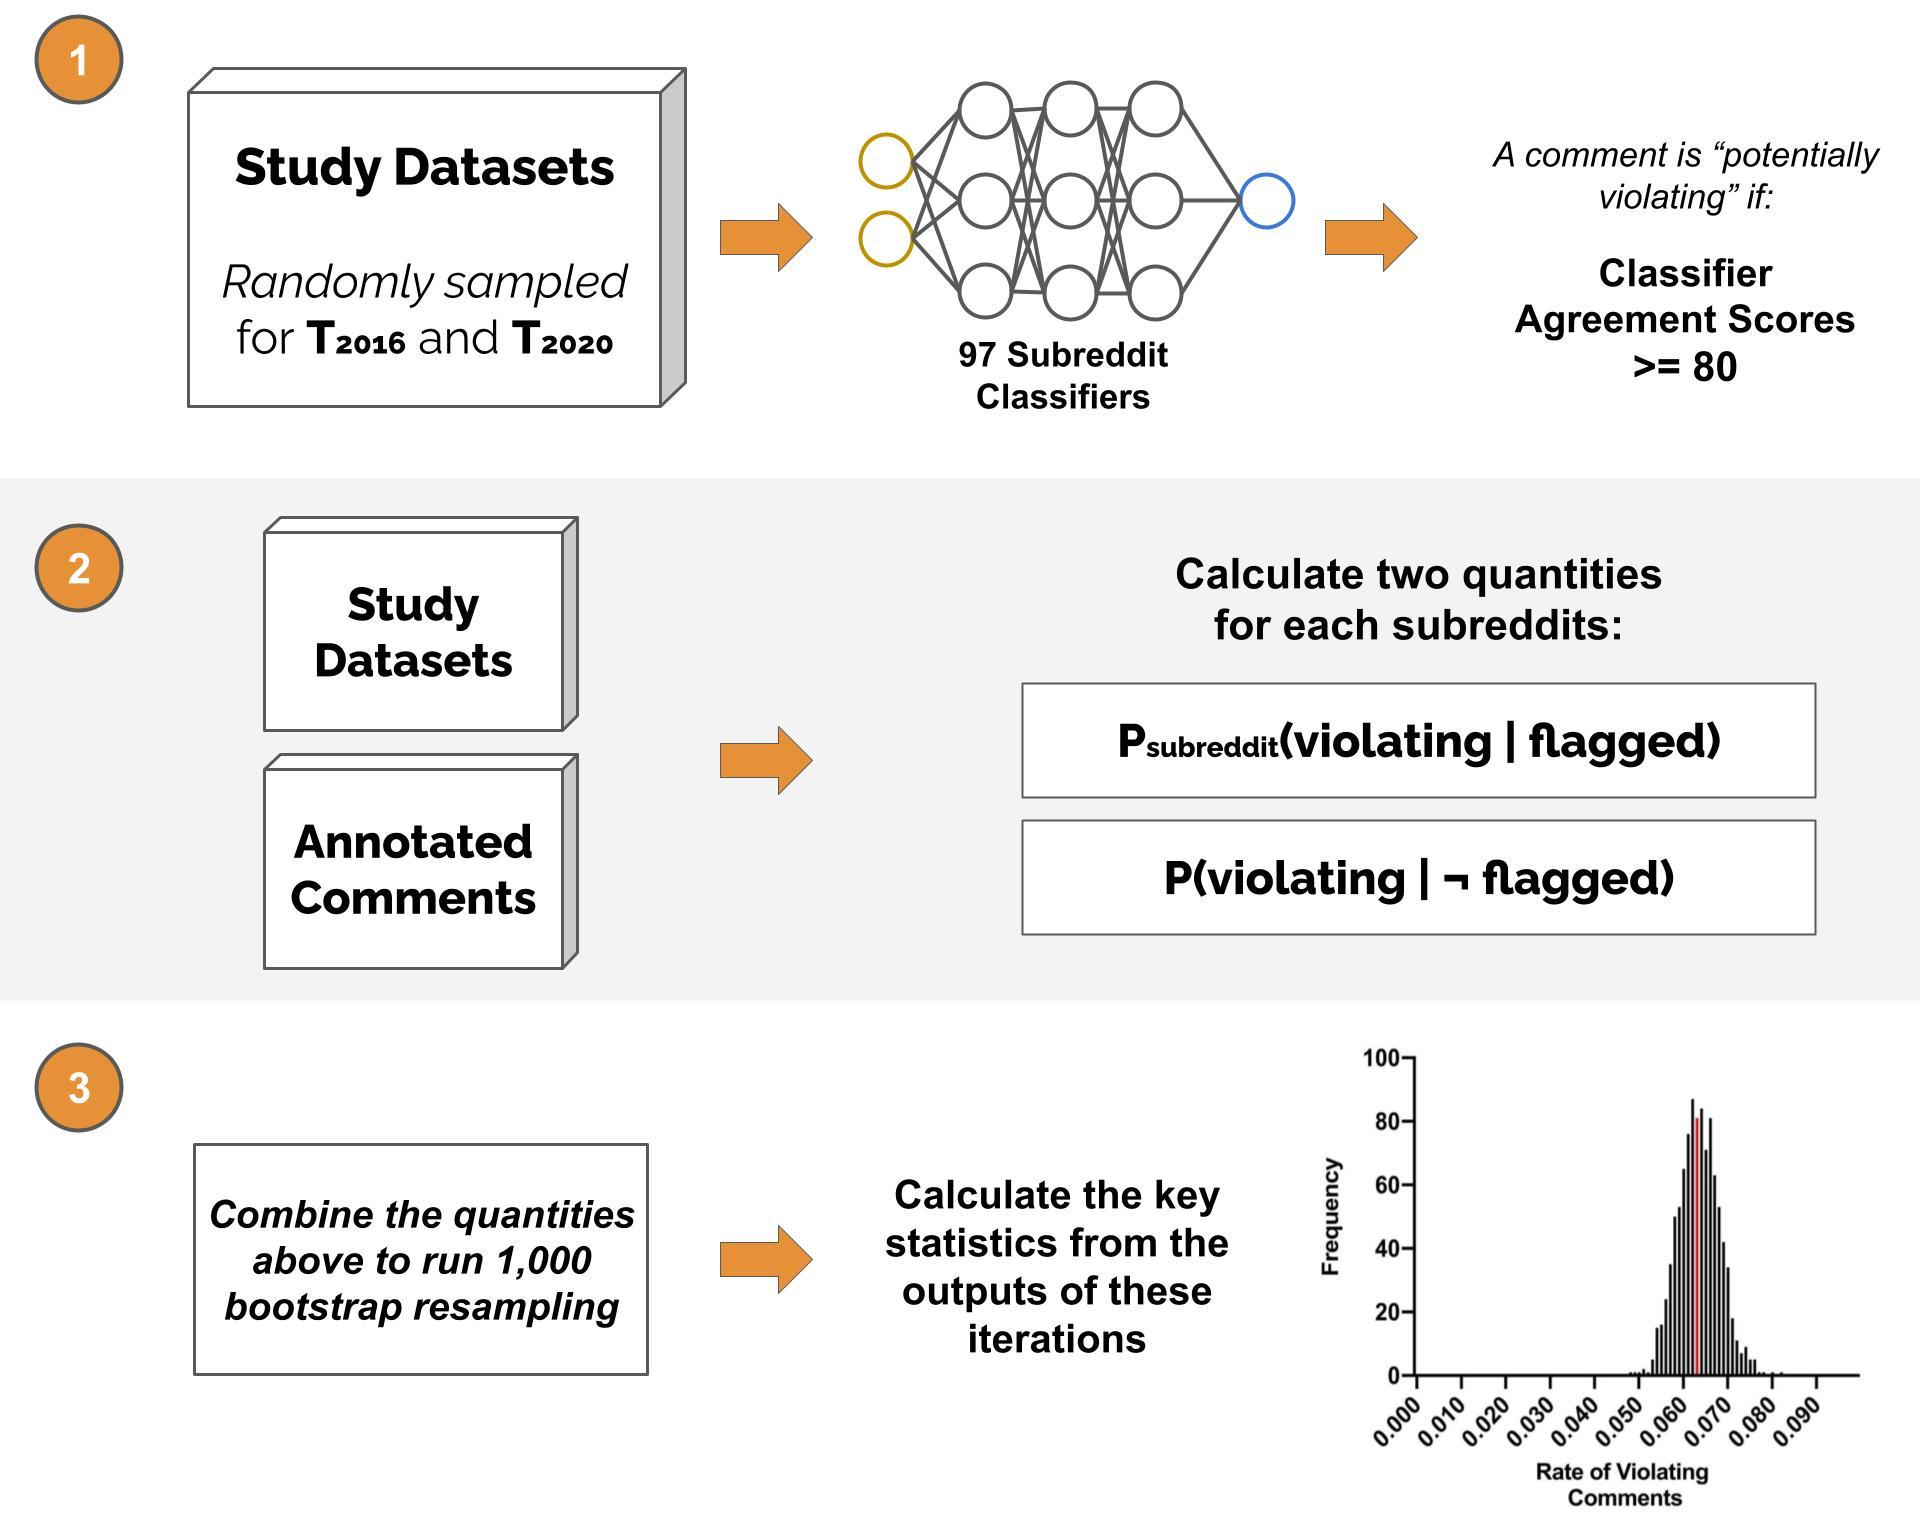
\includegraphics[width=1.0\textwidth]{content_minor_revision__Apr2022/images/bootstrap_workflow_6.jpg}
  \caption{\rnr{An overview of the sampling process in broad strokes. We start by randomly sampling unmoderated comments from $T_{2016}$ and $T_{2020}$ to generate our study datasets. We then use these datasets and the annotated comments to calculate key quantities that are needed for our bootstrap resampling. We then combine these quantities to implement our resampling procedure, which we repeat 1,000 times for each time periods of our interest.}}
  \label{fig:bootstrap}
  \Description{Bootstrap resampling workflow}
\end{figure}
\begin{figure}[tb]
  \centering
  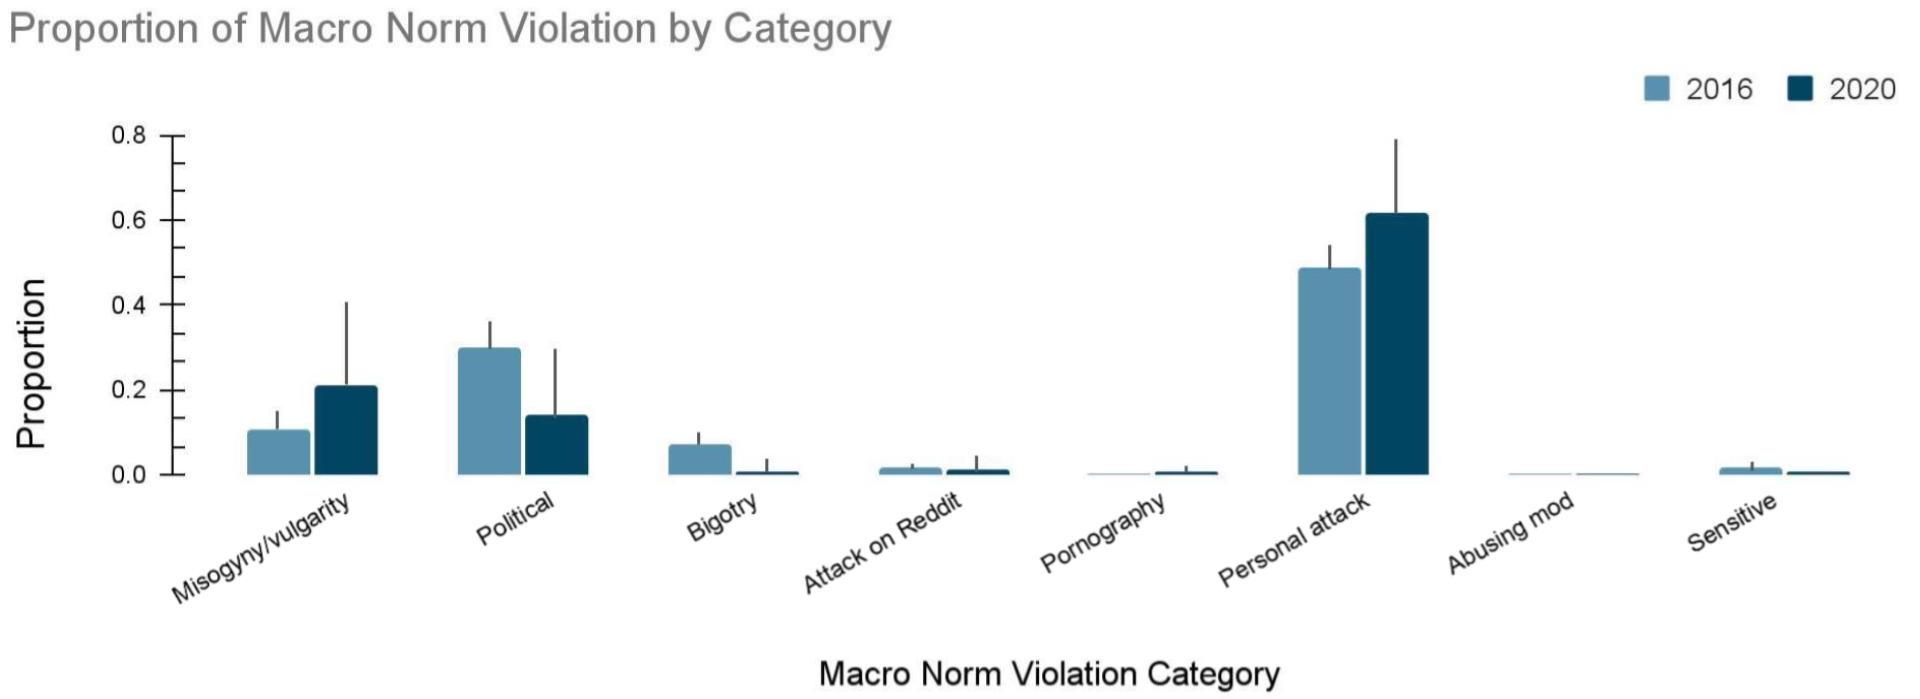
\includegraphics[width=1\textwidth]{content_minor_revision__Apr2022/images/macro_norm_violation_fixed_2.jpg}
  \caption{The proportion of macro norm violation by the eight categories among the unmoderated problematic comments according to our annotators. In $T_{2016}$ as well as $T_{2020}$, personal attacks were the most common macro norm violations. Politically inflammatory comments, on the other hand, have become less prevalent.}
  \Description{Proportion of Macro Norm Violation by Categories}
\end{figure}
% THIS HAS TO BE WITH 6.2.1


\begin{figure}[tb]
  \centering
  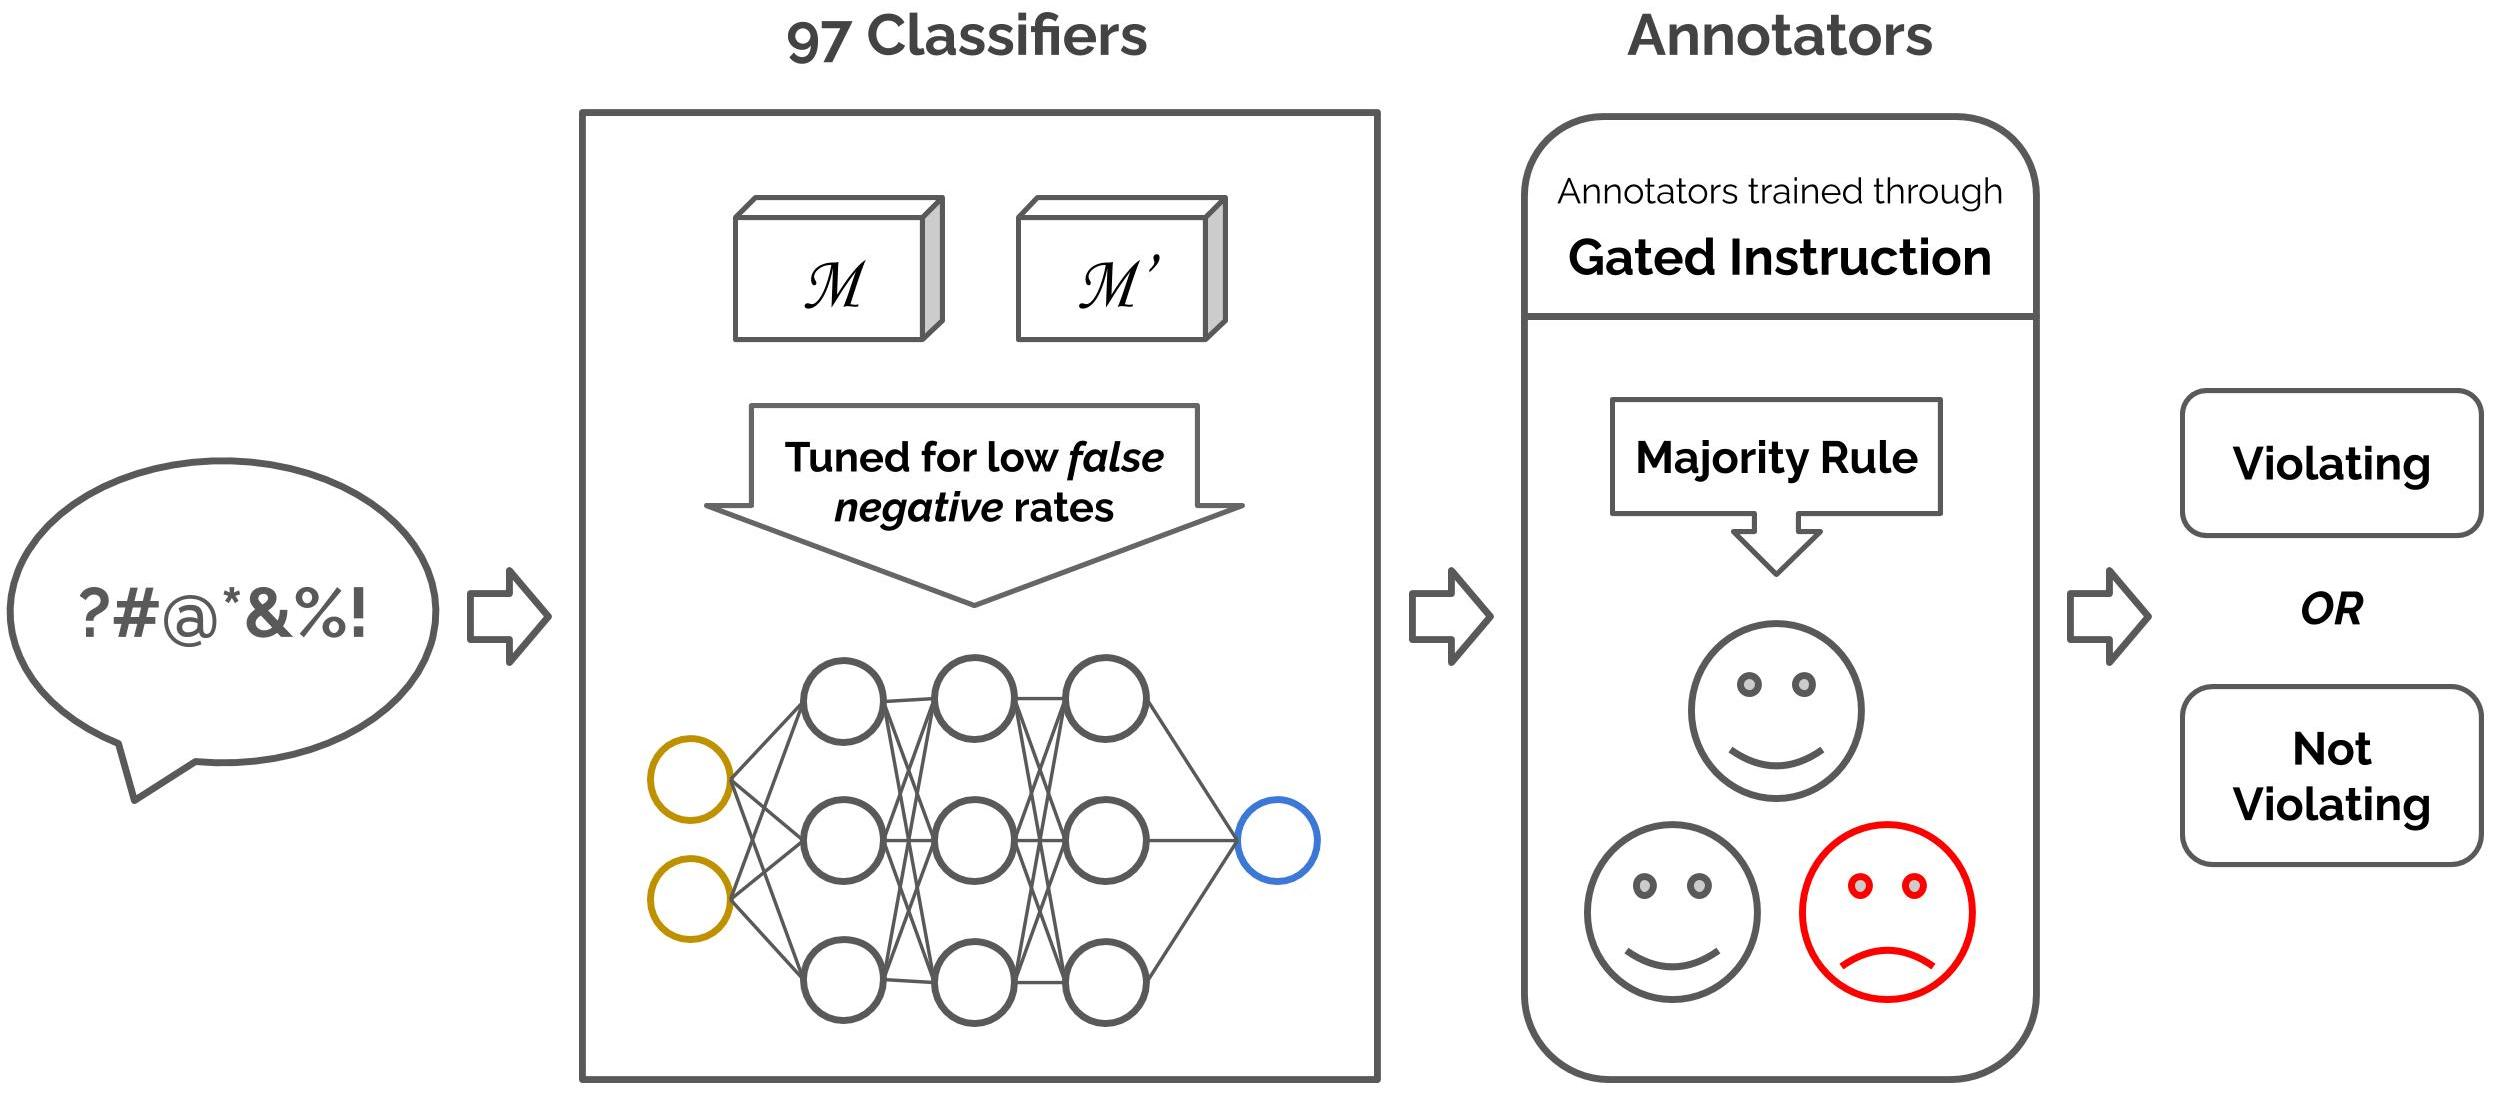
\includegraphics[width=0.90\textwidth]{content_minor_revision__Apr2022/images/Final_pipeline.jpg}
  \caption{An illustration of the human-AI pipeline for identifying violating comments. Our pipeline includes 97 subreddit classifiers that are trained using a balanced dataset of moderated and unmoderated comments, and human annotators who are trained through gated instruction~\cite{25_Liu}. Our classifiers (tuned for high recall) nominate potentially violating comments and human annotators make the final determination.}
  \Description{Human-AI pipeline}
\end{figure}


\begin{figure}[tb]
  \centering
  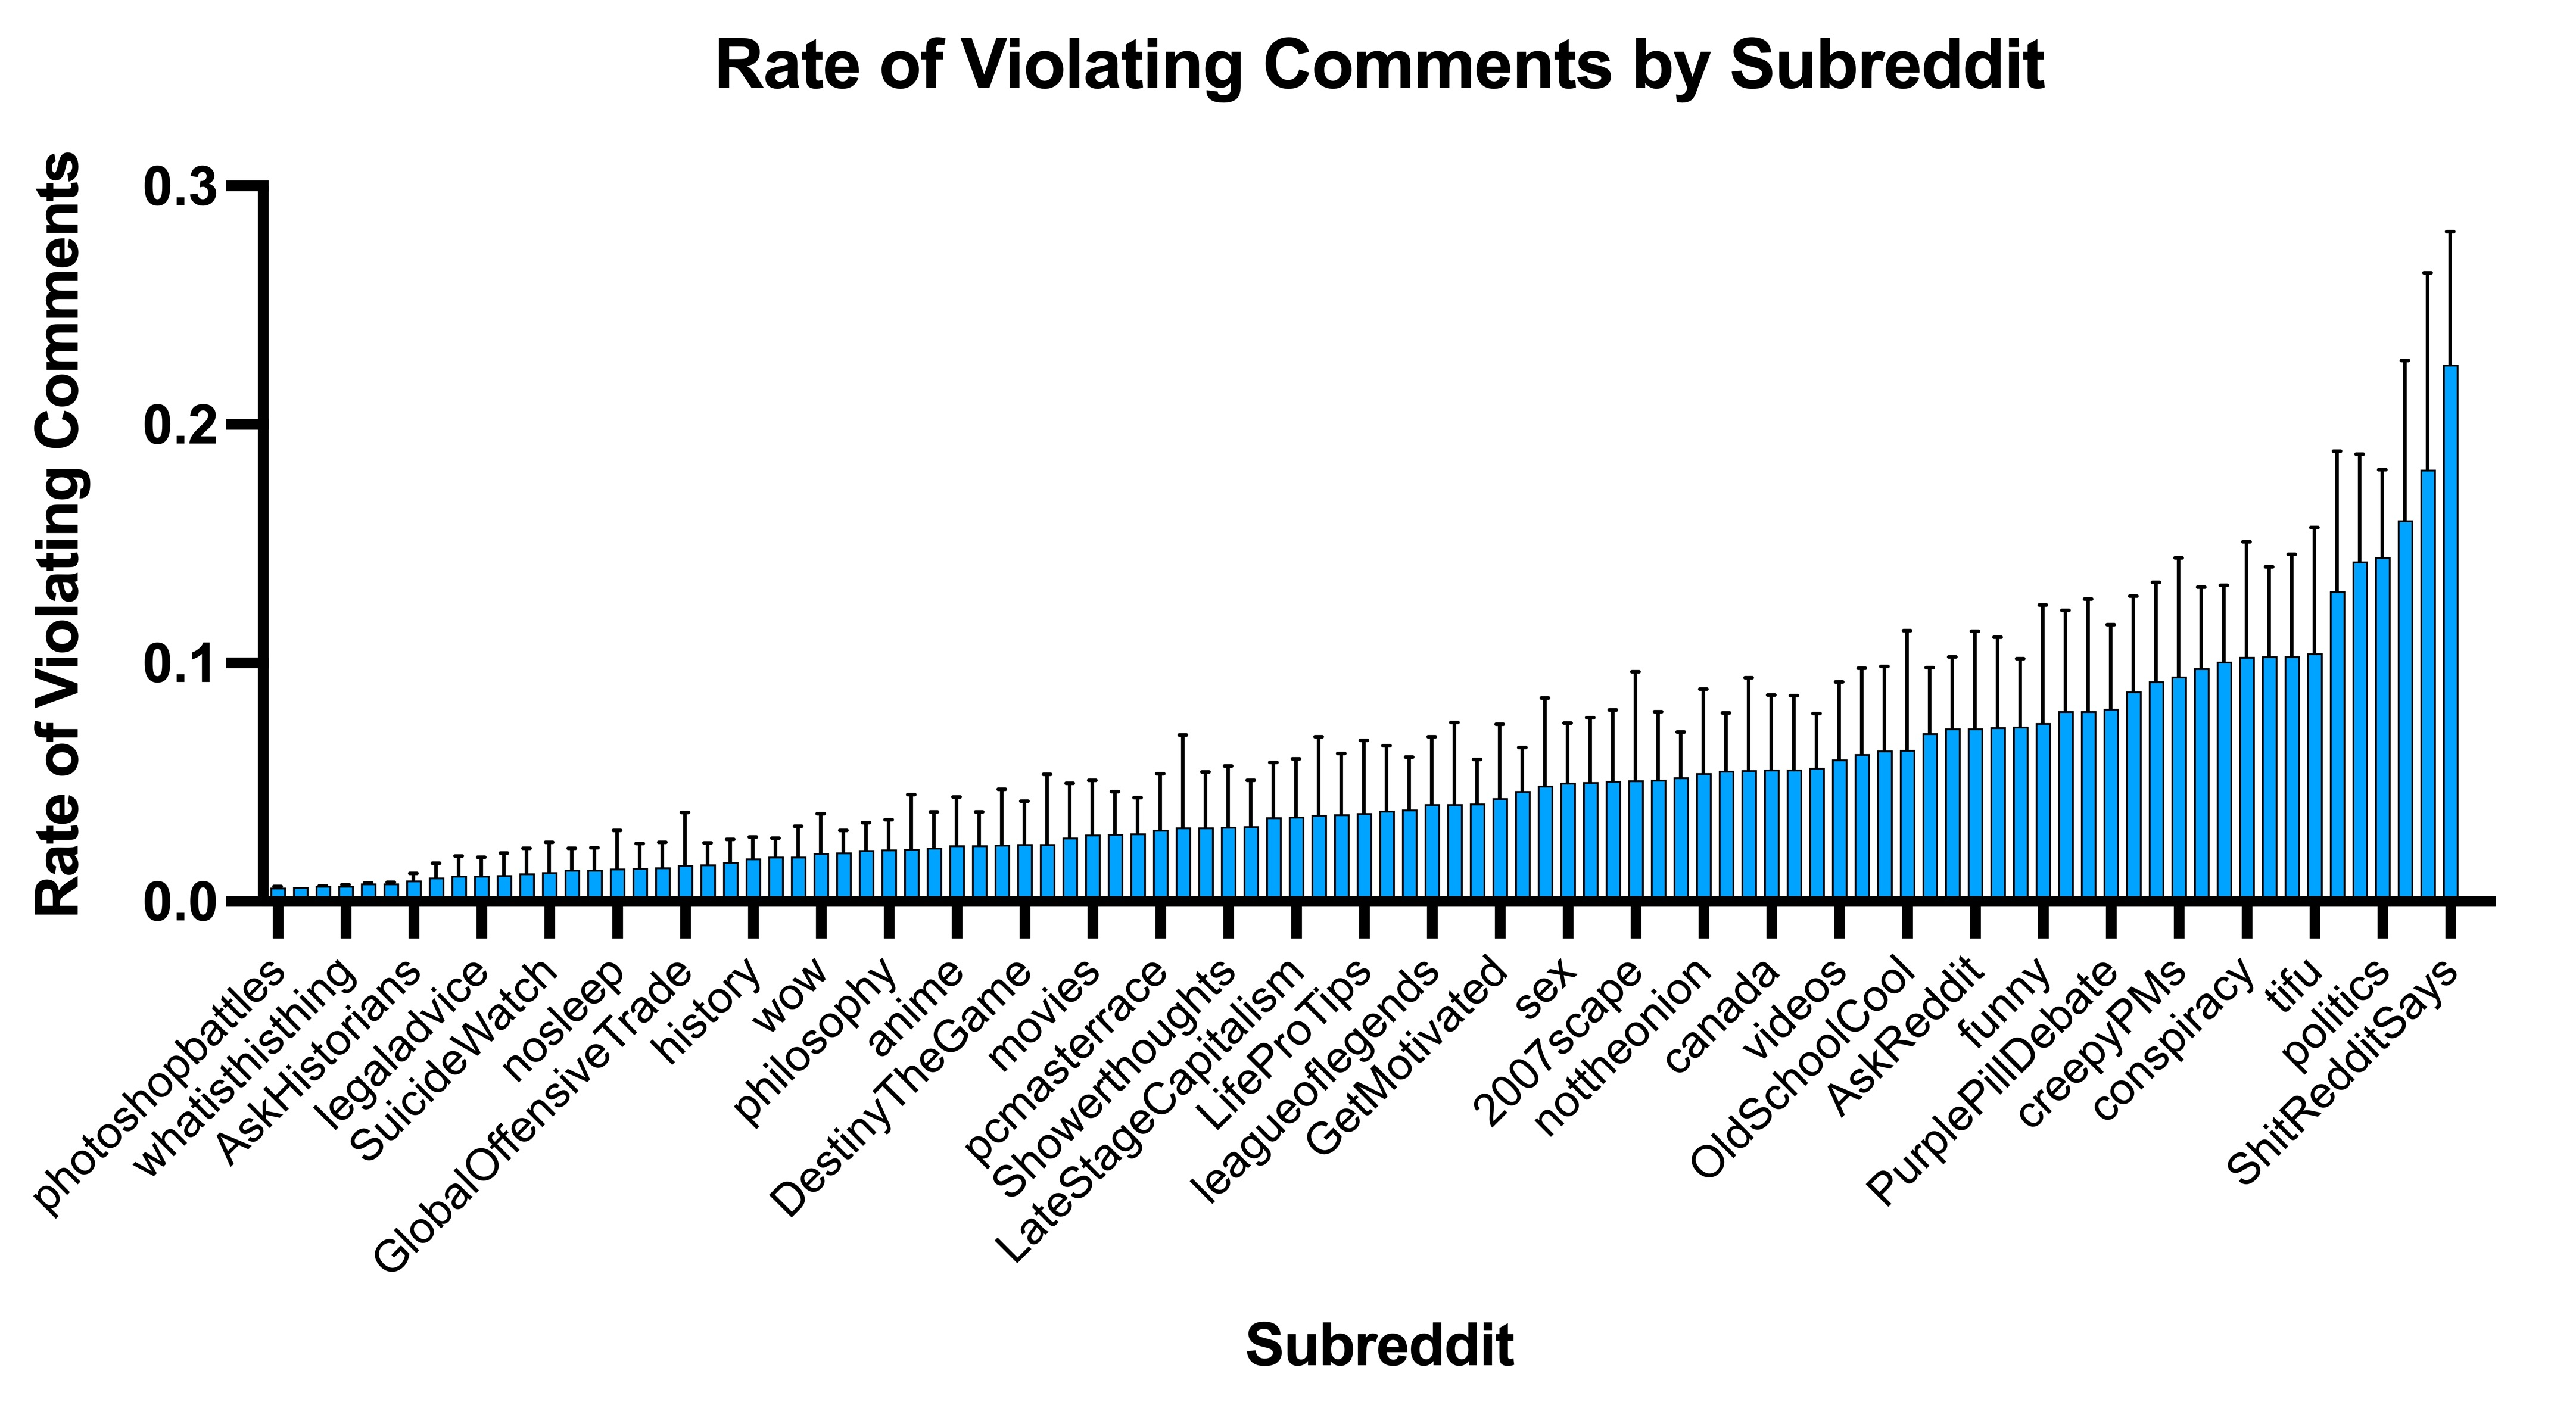
\includegraphics[width=0.95\textwidth]{content_minor_revision__Apr2022/images/all_rate_of_violating.jpg}
  \caption{Rate of \rnr{macro norm} violating comments by subreddit in $T_{2016}$. The lighter lines indicate 95\% confidence intervals. Subreddits vary in levels of violating content; some subreddits like r/depression (1.10\%) and r/Android (1.42\%) contain almost no  \rnr{violating} comments online, whereas some like r/creepyPMs (9.42\%) and r/EnoughTrumpSpam (14.27\%) contains much higher rates of \rnr{violating} comments.}
  \Description{Rate of macro norm violating comments by subreddits}
\end{figure}

\begin{figure}[tb]
  \centering
  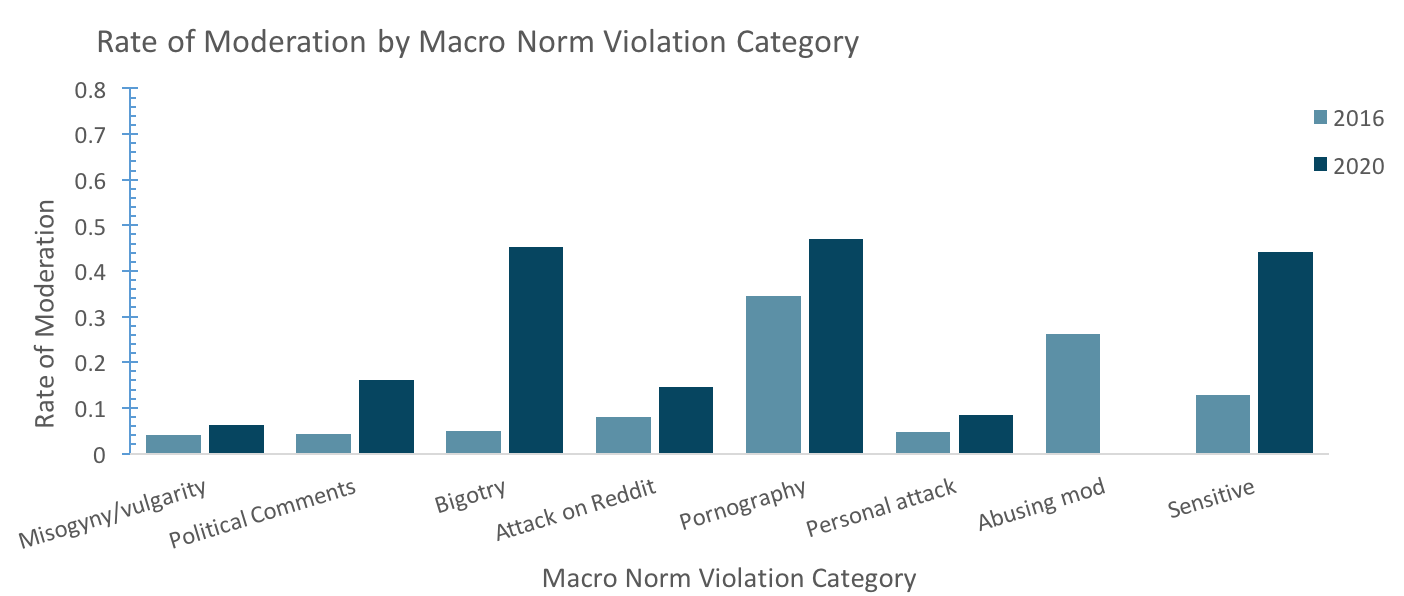
\includegraphics[width=1\textwidth]{content_minor_revision__Apr2022/images/ef_MODERATION.png}
  \caption{The rate of moderation by the eight macro norm violation categories acquired through stratified sampling. In $T_{2016}$, comments that contain links to pornography and comments that abuse or criticize moderators were moderated at the highest rate. In $T_{2020}$, comments with links to pornography is still among the most commonly moderated categories of norm violation. In addition, the overall rate of moderation has increased.  }
  \Description{Rate of moderation by macro norm violation categories}
\end{figure}
% THIS HAS TO BE WITH 6.2.2. AND COME AFTER PROPORTION... 


\begin{figure}[tb]
  \centering
  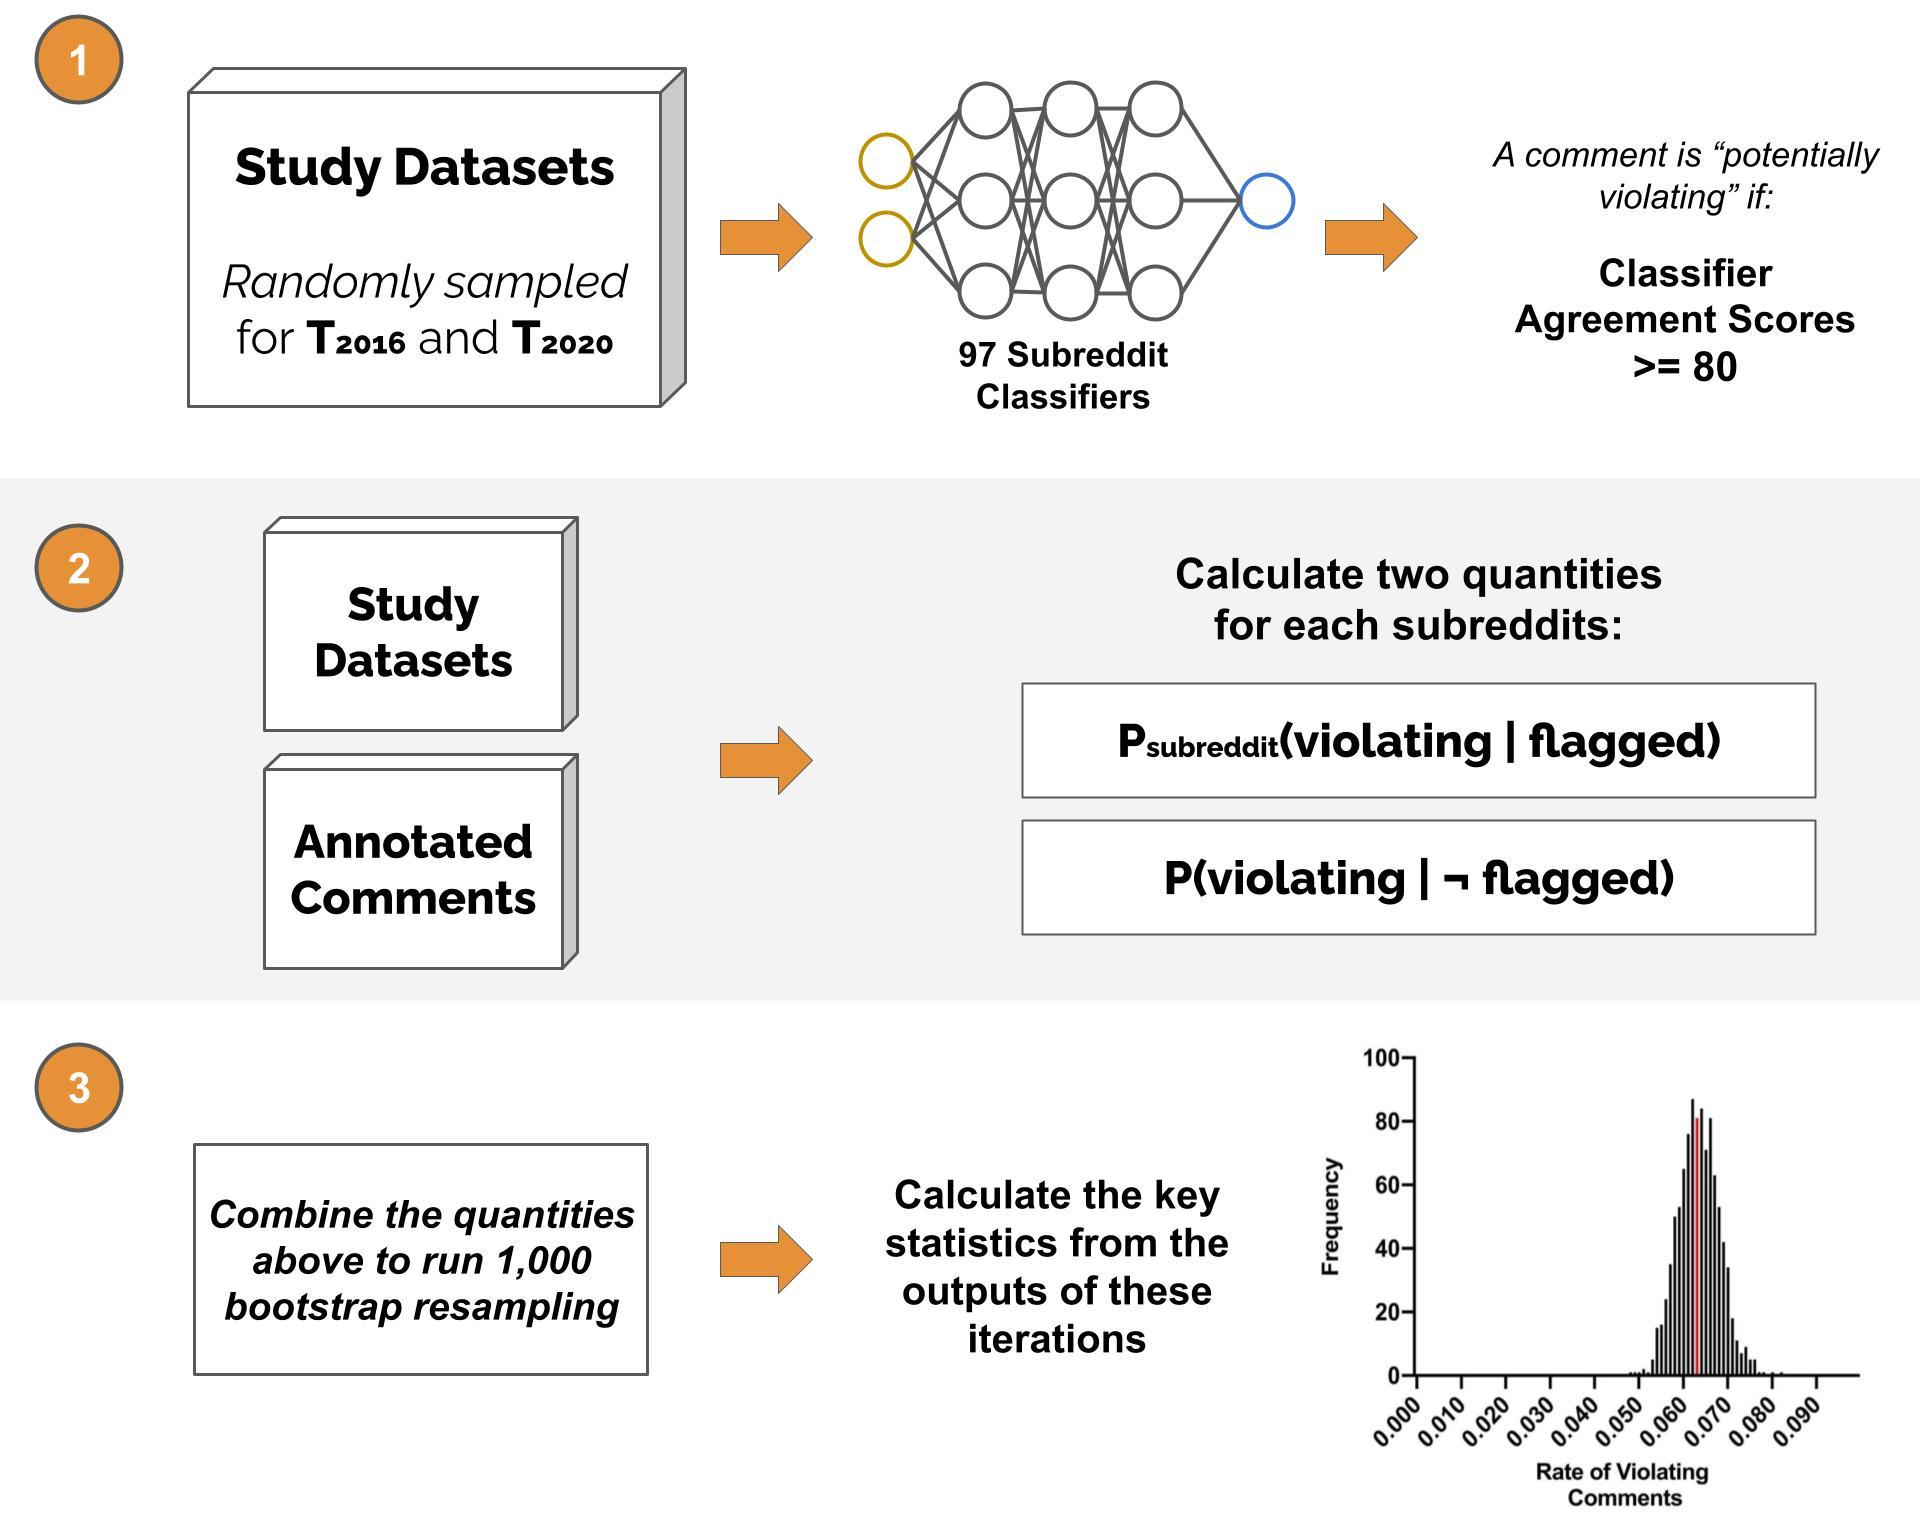
\includegraphics[width=1.0\textwidth]{content_minor_revision__Apr2022/images/bootstrap_workflow_6.jpg}
  \caption{\rnr{An overview of the sampling process in broad strokes. We start by randomly sampling unmoderated comments from $T_{2016}$ and $T_{2020}$ to generate our study datasets. We use these datasets and the annotated comments to calculate key quantities needed for our bootstrap resampling. We then combine these quantities to implement our resampling procedure, which we repeat 1,000 times for each time periods of our interest.}}
  \label{fig:bootstrap}
  \Description{Bootstrap resampling workflow}
\end{figure}

\begin{figure}[tb]
  \centering
  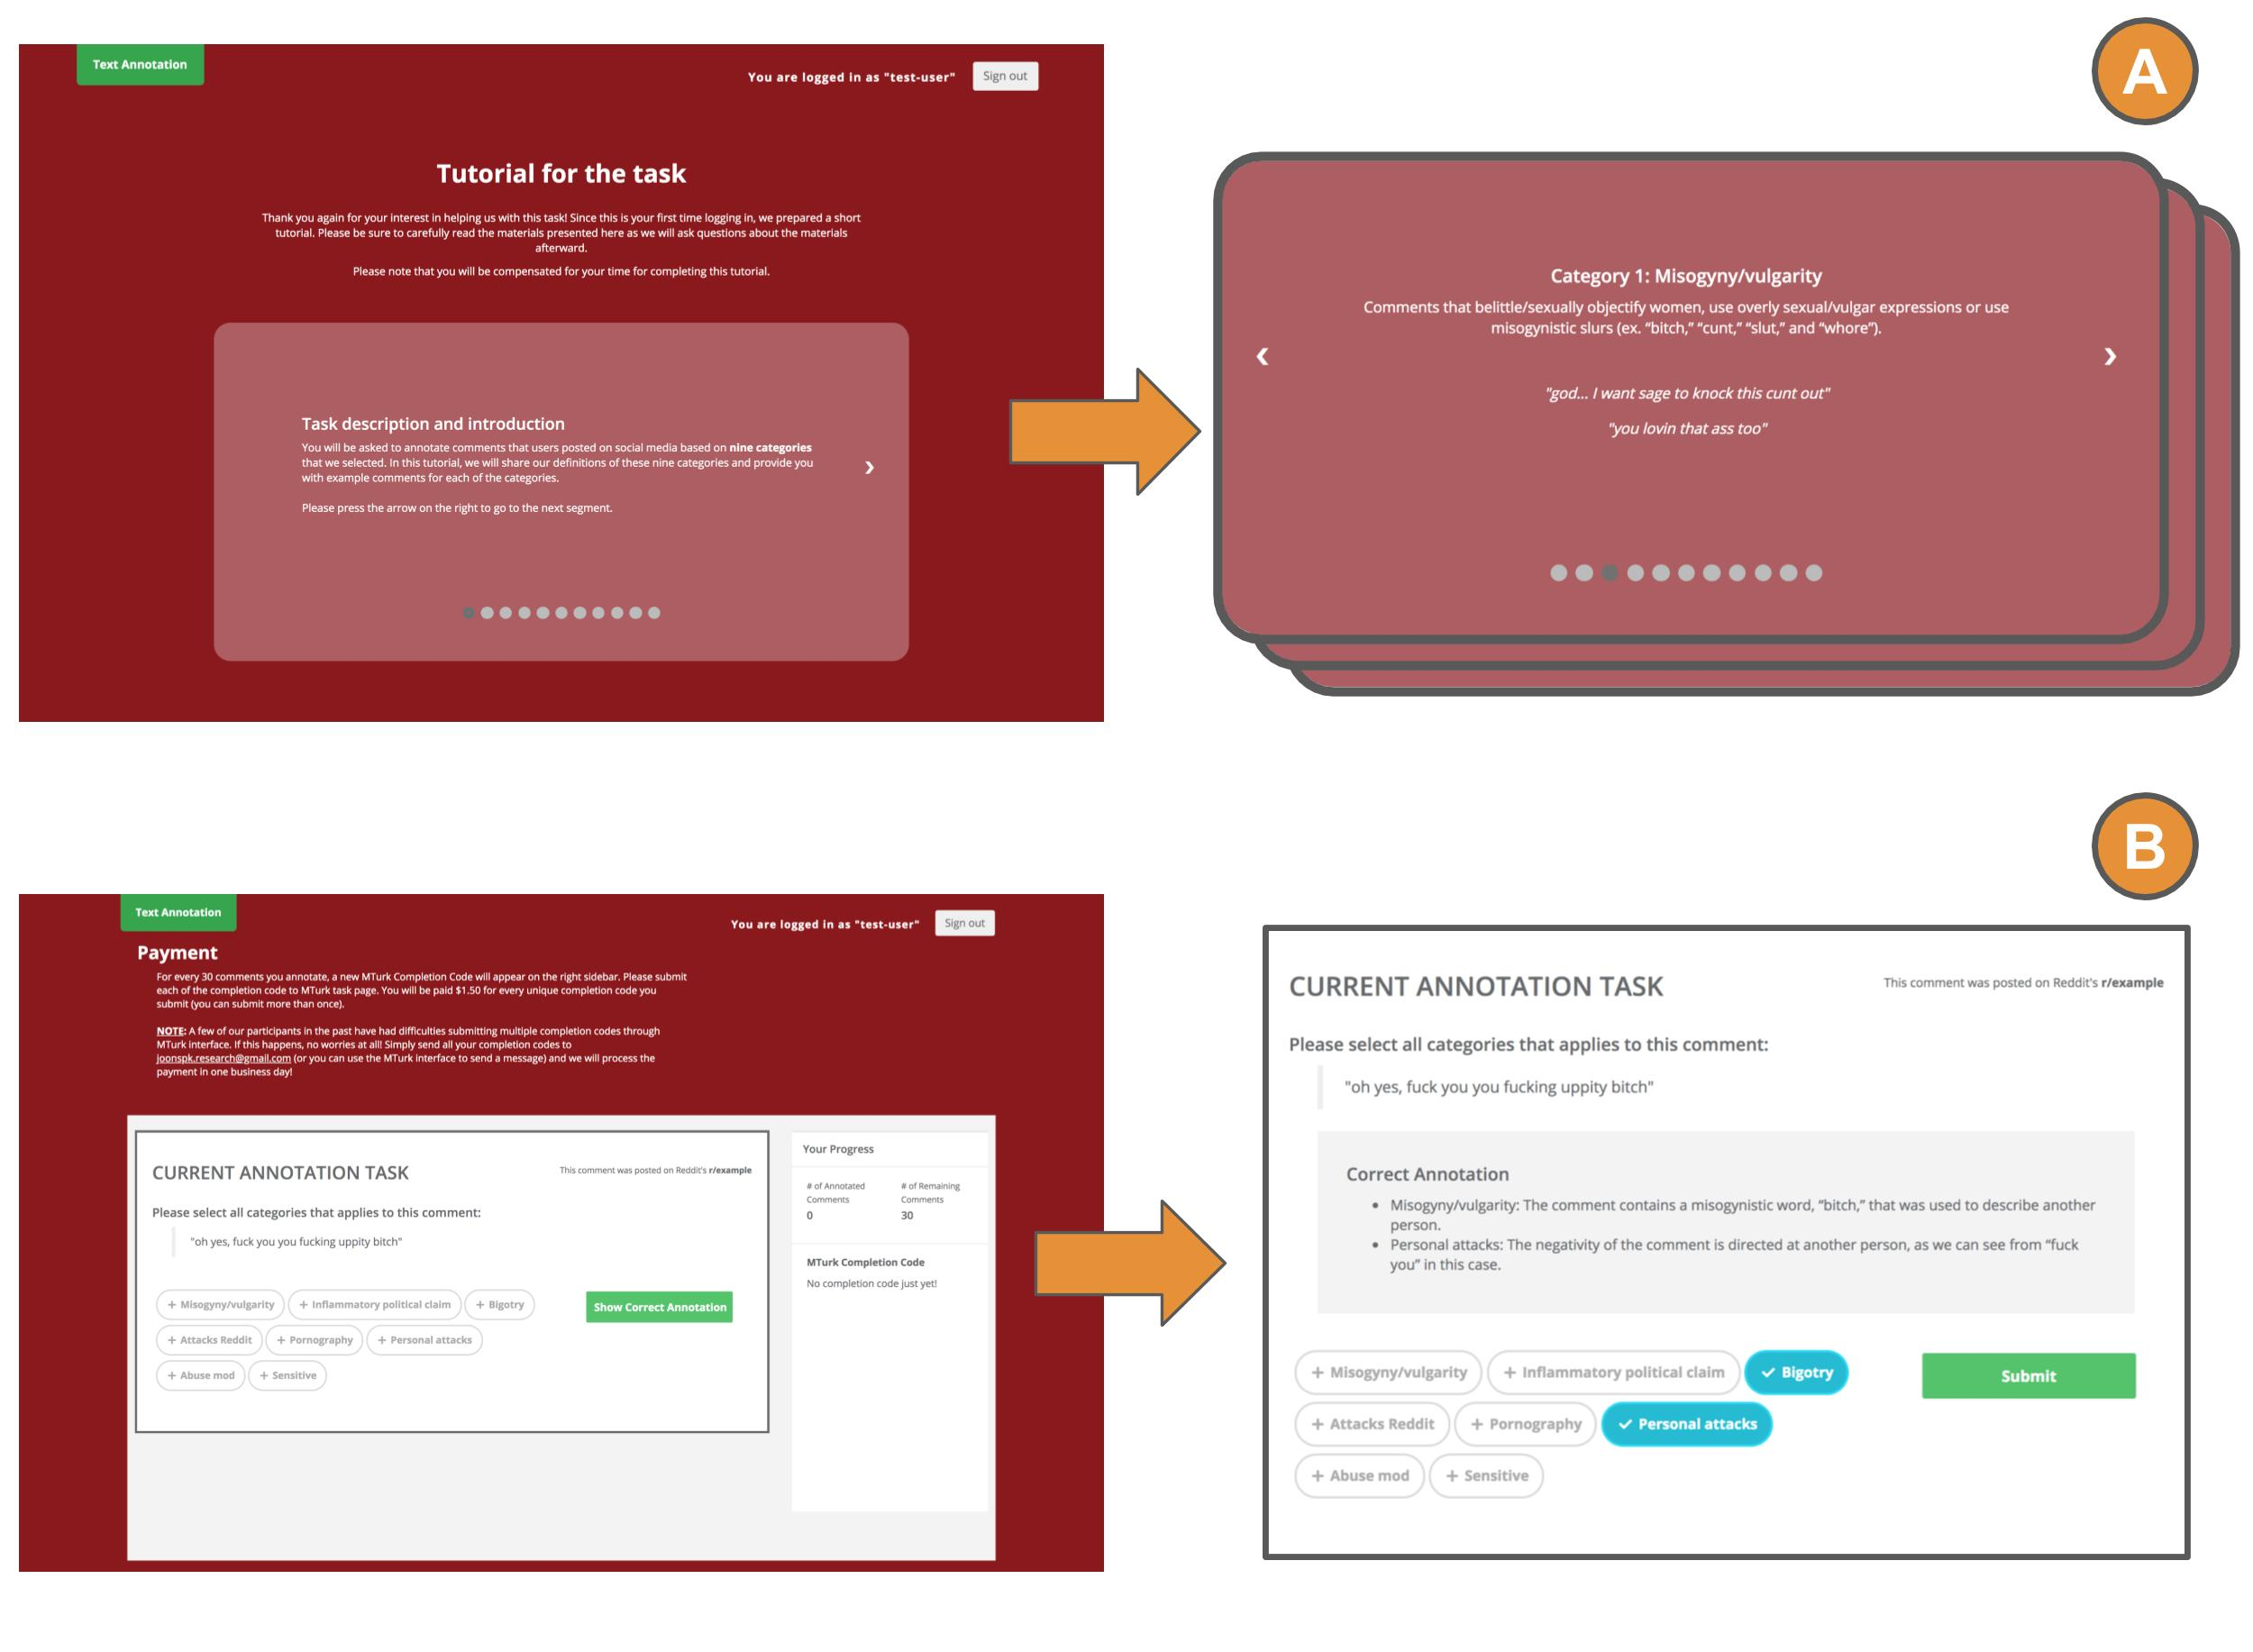
\includegraphics[width=0.98\textwidth]{content_minor_revision__Apr2022/images/annotation_interface.jpg}
  \caption{\textbf{A:} The interface for introducing the task description and eight macro norms to a new annotator. The definitions for each norms are shown one by one, accompanied by gold-standard examples that violate the norm. \textbf{B:} The interface for training and testing new annotators. Once the new annotators select their annotation, the correct annotation is shown accompanied by gold-standard examples. The interface for the main annotation task is the same but without presenting the correct annotation portion.}
  \Description{Annotation Interface}
\end{figure}



\begin{figure}[tb]
  \centering
  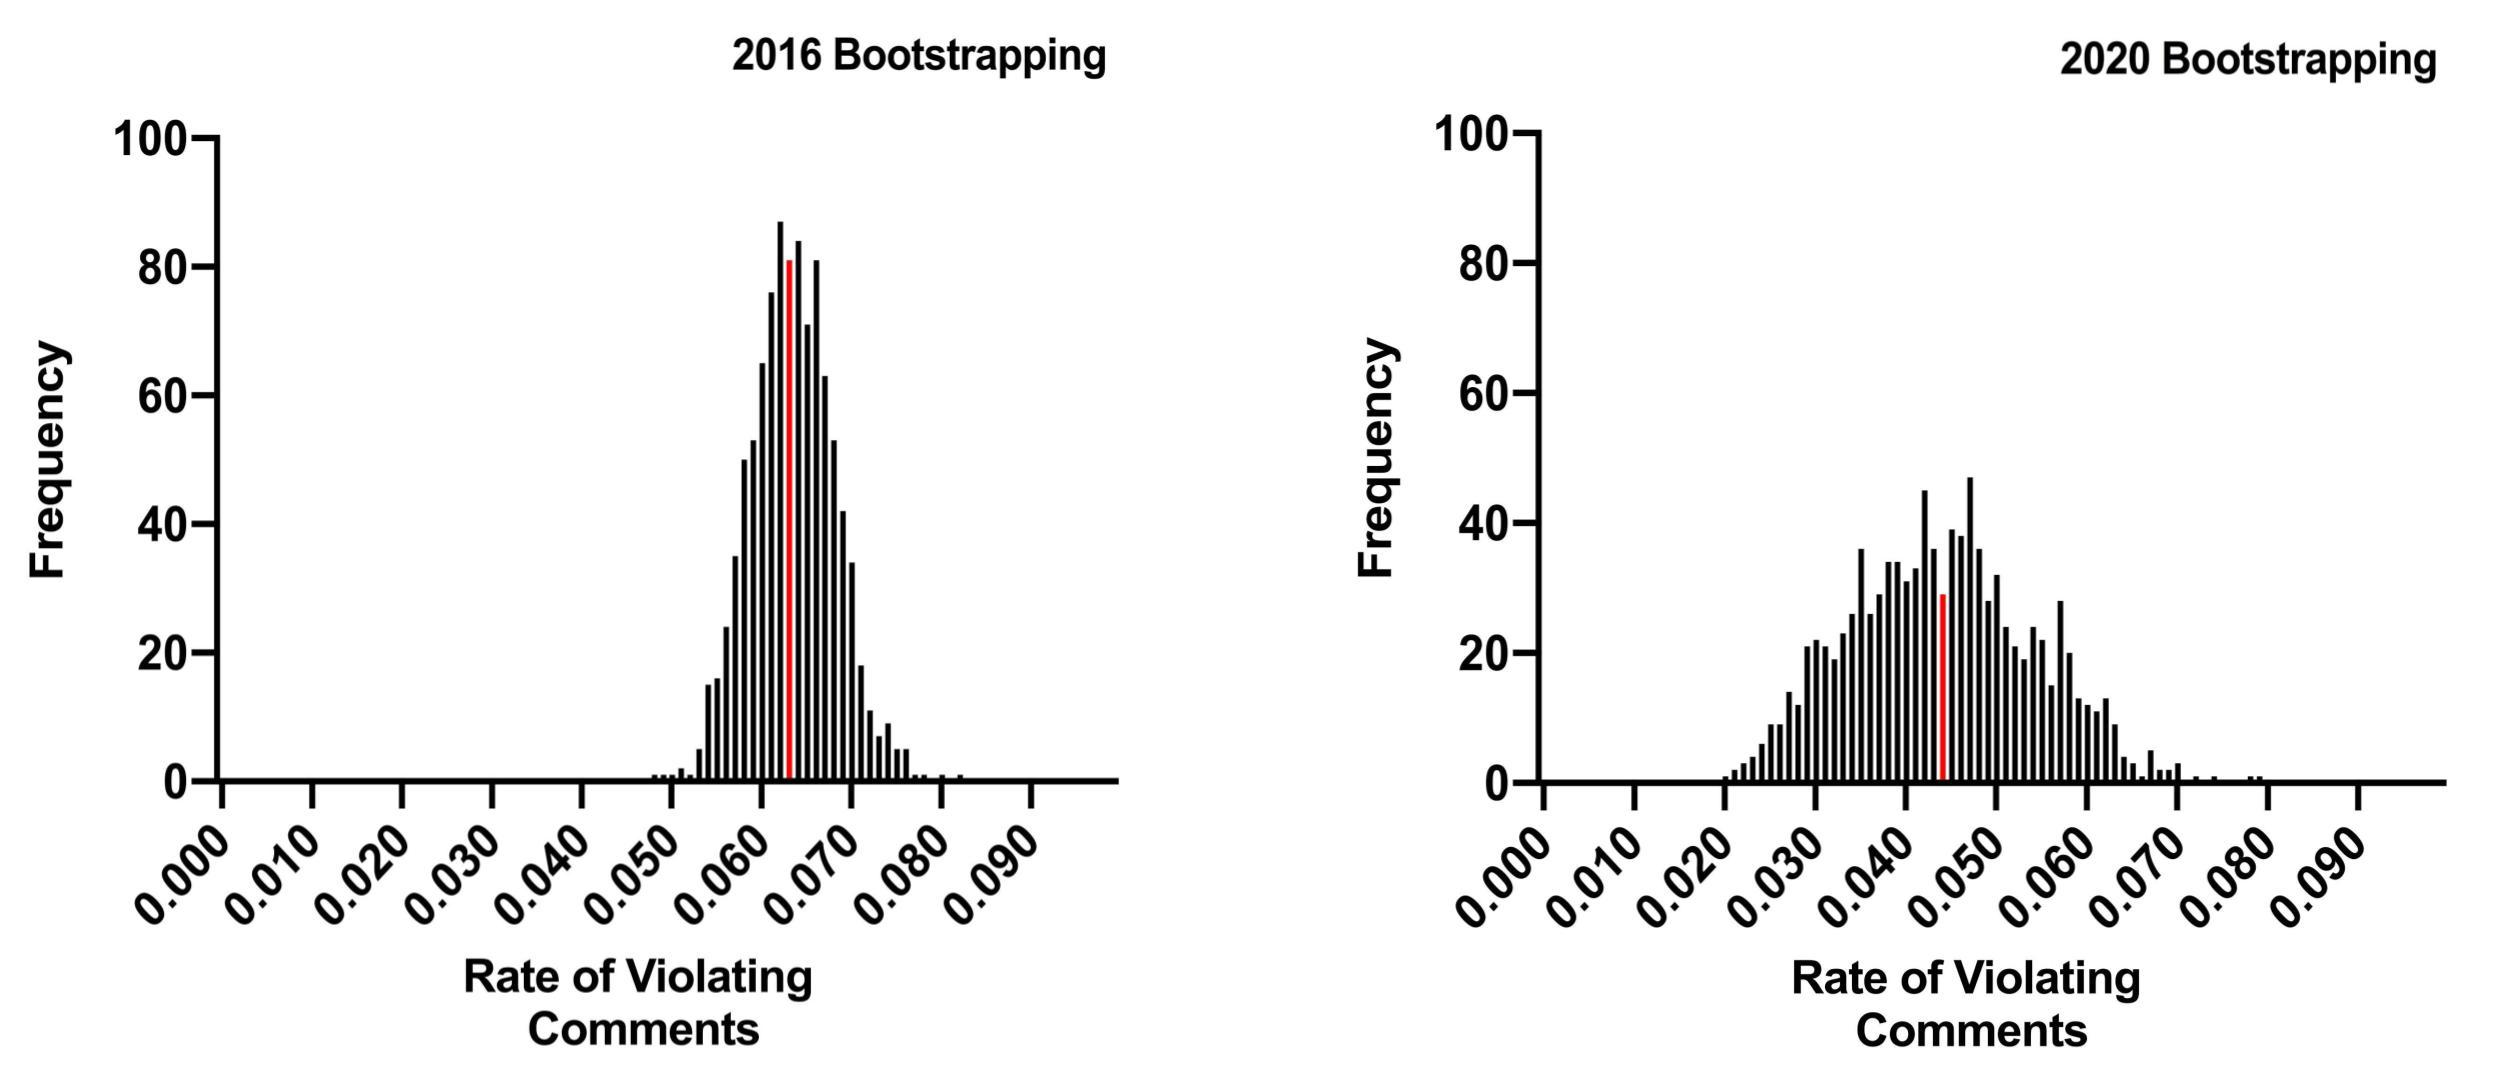
\includegraphics[width=0.95\textwidth]{content_minor_revision__Apr2022/images/bootstrap_rate.jpg}
  \caption{The results of our bootstrap sampling. The figures show the overall rates of violating comments that are left unmoderated for all 1,000 simulations of Reddit for $T_{2016}$ and $T_{2020}$. The 50th percentile rates for the 1,000 bootstrap samples are colored red for the two periods.}
  \label{fig:bootstraprate}
  \Description{Annotation Interface}
\end{figure}

% \usepackage{booktabs}


% \usepackage{booktabs}


\begin{table}[tb]
\centering
\caption{Parameters and the values used for them to fine-tune the classifiers}
\begin{tabular}{ll}
\multicolumn{1}{c}{\textbf{DESCRIPTION} } & \multicolumn{1}{c}{\textbf{SET OF VALUES} }  \\ 
\toprule
Size of the word index                    & {[}10000, 44000]                             \\
Max length of the input                   & {[}256, 512]                                 \\
Number of epochs during the training      & {[}30, 40, 50]                               \\
\# of nodes for the ReLU layer            & {[}16, 32]                                   \\
\bottomrule
\end{tabular}
\end{table}

% \begin{table}
% \centering
% \caption{Parameters and the values used for them to fine-tune the classifiers}
% \begin{tabular}{lll}
% \multicolumn{1}{c}{\textbf{PARAMETERS}} & \multicolumn{1}{c}{\textbf{DESCRIPTION}} & \multicolumn{1}{c}{\textbf{SET OF VALUES}}  \\ 
% \toprule
% \textit{$\mathcal{WI}$}                             & Size of the word index                   & {[}10000, 44000]                            \\
% \textit{$\mathcal{ML}$}                             & Max length of the input                  & {[}256, 512]                                \\
% Epochs                                  & Number of epochs during the training     & {[}30, 40, 50]                              \\
% \textit{$\mathcal{DN}$}                             & \# of nodes for the ReLU layer           & {[}16, 32]                                  \\
% \bottomrule
% \end{tabular}
% \end{table}
% \usepackage{booktabs}




\begin{table}[tb]
\centering
\captionof{table}{The results of Poisson regression that predicts the rate of problematic comments in a subreddit. We find that the number of comments in a subreddit, as well as a few of the topic categories are strong predictors of the rate of problematic comments a subreddit may have. The topic "general content", which was included in the model, is not shown as it was used as the baseline dummy variable for the categorical variable.}
\begin{tabular}{lllll} 
\toprule
                               & \textbf{Coefficient} & \textbf{SE} & \textbf{z-score} & \textbf{p-value}  \\ 
\toprule
Intercept                      & -5.919               & 1.249       & -4.740           & < 0.001 (***)      \\
log(mod to comment ratio)      & -0.728               & 0.244       & -2.986           & 0.003 (**)        \\
Topic: Hobbies and Occupations & -2.048               & 0.280       & -7.304           & < 0.001 (***)      \\
Topic: NSFW                    & 1.958                & 0.253       & 7.742            & < 0.001 (***)      \\
Topic: Discussion              & -1.021               & 0.421       & -2.423           & 0.015 (*)         \\
Topic: Politics                & 0.628                & 0.260       & 2.414            & 0.016 (*)         \\
Topic: Humor                   & 0.408                & 0.251       & 1.621            & 0.105             \\
Topic: Lifestyle               & 0.0879               & 0.321       & 0.271            & 0.787             \\
Topic: Educational             & -1.191               & 0.647       & -1.840           & 0.078             \\
Topic: Entertainment           & -0.165               & 0.285       & -0.579           & 0.563             \\
Topic: Technology              & -0.387               & 0.325       & -1.191           & 0.233             \\
Topic: Other                   & 0.692                & 0.324       & 2.135            & 0.033             \\
\bottomrule
\end{tabular}
\end{table}

% \usepackage{caption}
% \usepackage{booktabs}
% \usepackage{arydshln}


\noindent\begin{minipage}{\linewidth}
\centering
\begin{tabular}{ll;{1pt/1pt}ll;{1pt/1pt}ll} 
\hline\hline
Subreddits         & \multicolumn{1}{l}{Count} & Subreddits           & \multicolumn{1}{l}{Count} & Subreddits          & Count  \\ 
\toprule
2007scape          & 8335                      & gameofthrones        & 7136                      & pcmasterrace        & 16986  \\
Android            & 10650                     & Games                & 28587                     & personalfinance     & 22841  \\
anime              & 8365                      & gaming               & 12270                     & philosophy          & 8710   \\
AskHistorians      & 28772                     & GetMotivated         & 5823                      & photoshopbattles    & 19620  \\
AskReddit          & 110k                      & gifs                 & 10075                     & pics                & 16921  \\
askscience         & 38851                     & GlobalOffensive      & 16340                     & pokemon             & 8759   \\
AskTrumpSupporters & 7039                      & GlobalOffensiveTrade & 12751                     & pokemongo           & 16789  \\
AskWomen           & 13192                     & gonewild             & 51012                     & pokemontrades       & 14144  \\
asoiaf             & 5817                      & hearthstone          & 6335                      & PoliticalDiscussion & 26360  \\
atheism            & 10538                     & hillaryclinton       & 39683                     & politics            & 148k   \\
aww                & 21222                     & hiphopheads          & 9279                      & PurplePillDebate    & 5852   \\
BlackPeopleTwitter & 14200                     & history              & 13554                     & relationships       & 52987  \\
books              & 9501                      & IAmA                 & 6030                      & SandersForPresident & 16012  \\
canada             & 7742                      & india                & 9688                      & science             & 105k   \\
CanadaPolitics     & 7529                      & jailbreak            & 5616                      & sex                 & 12873  \\
CFB                & 17108                     & LateStageCapitalism  & 12303                     & ShitRedditSays      & 7798   \\
changemyview       & 8034                      & leagueoflegends      & 33035                     & Showerthoughts      & 11531  \\
Christianity       & 8578                      & legaladvice          & 13813                     & socialism           & 7720   \\
churning           & 8044                      & LifeProTips          & 6827                      & space               & 7976   \\
conspiracy         & 7920                      & me\_irl              & 6075                      & spacex              & 6148   \\
creepyPMs          & 6941                      & MMA                  & 15546                     & SubredditDrama      & 6811   \\
dataisbeautiful    & 5922                      & movies               & 9720                      & SuicideWatch        & 6914   \\
depression         & 9500                      & nba                  & 8629                      & syriancivilwar      & 19618  \\
DestinyTheGame     & 5982                      & NeutralPolitics      & 5679                      & technology          & 6768   \\
DIY                & 11187                     & news                 & 76660                     & television          & 5963   \\
EnoughTrumpSpam    & 14203                     & nfl                  & 14630                     & TheSilphRoad        & 6629   \\
europe             & 15261                     & nosleep              & 18335                     & tifu                & 8084   \\
explainlikeimfive  & 56100                     & nottheonion          & 7442                      & TwoXChromosomes     & 51083  \\
fantasyfootball    & 8149                      & NSFW\_GIF            & 5921                      & UpliftingNews       & 10521  \\
food               & 9960                      & OldSchoolCool        & 7048                      & videos              & 13510  \\
funny              & 16344                     & OutOfTheLoop         & 10573                     & whatisthisthing     & 11691  \\
Futurology         & 16213                     & Overwatch            & 8131                      & worldnews           & 95026  \\
wow                & \multicolumn{1}{l}{6896}  &                      & \multicolumn{1}{l}{}      &                     &        \\
\midrule

\end{tabular}
\captionof{table}{\rnr{The size of the moderated comment datasets per subreddit that were used to train the subreddit classifiers. In addition to the moderated comments, we gathered the same number of unmoderated comments for each of the subreddits to create a balanced dataset for training the classifiers.}}

\end{minipage}
% \usepackage{booktabs}
% \usepackage{vcell}


\begin{table}[tb]
\centering
\caption{The eight macro norm violations on 97 popular subreddits and their definitions. We took the norms uncovered in a prior study \cite{Chandrasekharan2018internet} and expanded on some of their definitions to better fit our data.}
\begin{tabular}{ll}
\multicolumn{1}{c}{\textbf{MACRO NORM VIOLATIONS}}                                                & \multicolumn{1}{c}{\textbf{EXAMPLE COMMENTS}}                                                                                                                                         \\ 
\toprule
\vcell{Using misogynistic or vulgar slurs}                                                        & \vcell{\textit{"god... I want sage to knock this c*** out"}}                                                                                                                          \\[-\rowheight]
\printcelltop                                                                                     & \printcelltop                                                                                                                                                                         \\
\vcell{Inflammatory political claims}                                                             & \vcell{\begin{tabular}[b]{@{}l@{}}\textit{"a day old troll complaining about liberals -- I }\\\textit{smell a lost trumpkin"}\end{tabular}}                                           \\[-\rowheight]
\printcelltop                                                                                     & \printcelltop                                                                                                                                                                         \\
\vcell{Bigotry}                                                                                   & \vcell{\begin{tabular}[b]{@{}l@{}}\textit{"punishment for not being hateful enough and }\\\textit{not destroying the gays"}\end{tabular}}                                             \\[-\rowheight]
\printcelltop                                                                                     & \printcelltop                                                                                                                                                                         \\
\vcell{\begin{tabular}[b]{@{}l@{}}Verbal attacks on Reddit or specific \\subreddits\end{tabular}} & \vcell{\begin{tabular}[b]{@{}l@{}}\textit{"also reddit sucks because a user making~an~error }\\\textit{refuses to delete their post and redo it }\\\textit{correctly"}\end{tabular}}  \\[-\rowheight]
\printcelltop                                                                                     & \printcelltop                                                                                                                                                                         \\
\vcell{Posting pornographic links}                                                                & \vcell{\textit{[URL]}}                                                                                                                                                                \\[-\rowheight]
\printcelltop                                                                                     & \printcelltop                                                                                                                                                                         \\
\vcell{Personal attacks}                                                                          & \vcell{\textit{"you know man youre kind of a f***ing d*****"}}                                                                                                                        \\[-\rowheight]
\printcelltop                                                                                     & \printcelltop                                                                                                                                                                         \\
\vcell{Abusing and criticizing moderators}                                                        & \vcell{\textit{"the mods in this sub need to wake the f*** up"}}                                                                                                                      \\[-\rowheight]
\printcelltop                                                                                     & \printcelltop                                                                                                                                                                         \\
\vcell{\begin{tabular}[b]{@{}l@{}}Claiming the other person is too \\sensitive\end{tabular}}      & \vcell{\textit{"get off the internet with your sensitive ass"}}                                                                                                                       \\[-\rowheight]
\printcelltop                                                                                     & \printcelltop                                                                                                                                                                         \\
\bottomrule
\end{tabular}
\end{table}
